 % The main file for CAMP reports
 % Don't put any content in here. 
 % Don't even include content files by using \input or \inlcude. 
 % Put your content to TEXT.TEX or include it there using \input.
 % Uses:
 %		SETTINGS.TEX	contains the settings for this document
 %		COMMANDS.TEX	contains commands which can be used while writing
 %		INFO.TEX			contains the author, title and so on for the cover
 %		COVER.TEX			formats the front cover of the document
 %		ABSTRACT.TEX	contains the abstract to be included (if needed)
 %		TEXT.TEX			contains the actual content of the document
 %		BIB.BIB				containt the BibTeX entries for the document
 
%% !!!!! IMPORTANT !!!!!
%% HAS TO BE COMPILED WITH -shell-escape


%% Draft document mode
%% Final document
\documentclass[11pt,a4paper,bibtotoc,idxtotoc,headsepline,footsepline,footexclude,BCOR12mm,DIV13]{scrbook}

%\documentclass[11pt,a4paper,bibtotoc,idxtotoc,headsepline,footsepline,footexclude,BCOR20mm,DIV10]{scrbook}
\usepackage[force,almostfull]{textcomp}
%\usepackage[pdftex]{graphicx}

% KOMA-Optionen:
%  bibtotoc: include bibliography in table of contents
%  idxtotoc: include index in table of contents
%  headsepline: use horizontalline under heading
%  BCOR: binding correcion (Bindungskorrektur) (e.g.: BCOR5mm)
%  DIV: Number of sheet sections (used for layout) (e.g.: DIV12) 



% include title and author information for the cover
% Set here the title, authors and other stuff to be used for the cover
% This file is used by MAIN.TEX

% set title, authors and stuff for the cover
\def\doctype{Master's thesis\\Robotics, Cognition, Intelligence}
\def\title{Realizing Online (Self-)Collision Avoidance Based on Inequality Constraints with Hierarchical Inverse Kinematics}
\def\titleGer{Realisierung von Selbstkollisionsvermeidungen auf Basis von Ungleichheitsbedingungen mit Hierarchisch Inverser Kinematik}
\def\author{Karsten Knese}
\def\date{April 14 2014}

% text to appear in the footer
\def\footertext{}

% include settings
% Included by MAIN.TEX
% Defines the settings for the CAMP report document

\renewcommand{\sectfont}{\normalfont \bfseries}        % Schriftart der Kopfzeile

% manipulate footer
\usepackage{scrpage2}
\pagestyle{scrheadings}
\ifoot[\footertext]{\footertext} % \footertext set in INFO.TEX
%\setkomafont{pagehead}{\normalfont\rmfamily}
\setkomafont{pagenumber}{\normalfont\rmfamily}

%% allow sophisticated control structures
\usepackage{ifthen}

% use Palatino as default font
\usepackage{palatino}

% enable special PostScript fonts
\usepackage{pifont}

% make thumbnails
\usepackage{thumbpdf}

%to use the subfigures
\usepackage{subfigure}


\usepackage{colortbl}


%% show program code\ldots
%\usepackage{verbatim}
%\usepackage{program}

%% enable TUM symbols on title page
\usepackage{styles/tumlogo}


\usepackage{multirow}

%% use colors
\usepackage{color}

%% make fancy math
\usepackage{amsmath}
\usepackage{amsfonts}
\usepackage{amssymb}
\usepackage{textcomp}
\usepackage{yhmath} % fr die adots 
%% mark text as preliminary
%\usepackage[draft,german,scrtime]{prelim2e}

%% create an index
\usepackage{makeidx}

% for the program environment
\usepackage{float}

%% load german babel package for german abstract
%\usepackage[german,american]{babel}
\usepackage[german,english]{babel}
\selectlanguage{english}

% use german characters as well
\usepackage[latin1]{inputenc}       % allow Latin1 characters

% use initals dropped caps - doesn't work with PDF
\usepackage{dropping}


\usepackage{styles/shortoverview}
%----------------------------------------------------
%      Graphics and Hyperlinks
%----------------------------------------------------

%% check for pdfTeX
\ifx\pdftexversion\undefined
 %% use PostScript graphics
 \usepackage[dvips]{graphicx}
 \DeclareGraphicsExtensions{.eps,.epsi}
 \graphicspath{{figures/}{figures/review}} 
 %% allow rotations
 \usepackage{rotating}
 %% mark pages as draft copies
 %\usepackage[english,all,light]{draftcopy}
 %% use hypertex version of hyperref
 \usepackage[hypertex,hyperindex=false,colorlinks=false]{hyperref}
\else %% reduce output size \pdfcompresslevel=9
 %% declare pdfinfo
 %\pdfinfo { 
 %  /Title (my title) 
 %  /Creator (pdfLaTeX) 
 %  /Author (my name) 
 %  /Subject (my subject	) 
 %  /Keywords (my keywords)
 %}
 %% use pdf or jpg graphics
 \usepackage[pdftex]{graphicx}
 \DeclareGraphicsExtensions{.jpg,.JPG,.png,.pdf,.eps}
 \graphicspath{{figures/}} 
 
 %% Load float package, for enabling floating extensions
 \usepackage{float}
 
 %% allow rotations
 \usepackage{rotating}
 %% use pdftex version of hyperref
 \usepackage[pdftex,colorlinks=false,linkcolor=black,citecolor=black,%
 anchorcolor=black,urlcolor=blue,bookmarks=true,%
 bookmarksopen=true,bookmarksopenlevel=0,plainpages=false%
 bookmarksnumbered=true,hyperindex=true,pdfstartview=%
 ]{hyperref}
%
%\usepackage[pdftex,colorlinks=false,linkcolor=red,citecolor=red,%
% anchorcolor=red,urlcolor=red,bookmarks=true,%
% bookmarksopen=true,bookmarksopenlevel=0,plainpages=false%
% bookmarksnumbered=true,hyperindex=false,pdfstartview=%
% ]{hyperref}
\fi


\setlength\parindent{0pt}
\parskip = \baselineskip

%% Fancy chapters
%\usepackage[Lenny]{fncychap}
\usepackage[Glenn]{fncychap}
%\usepackage[Bjarne]{fncychap}

%\usepackage[avantgarde]{quotchap}

% set the bibliography style
%\bibliographystyle{styles/bauermaNum}
%\bibliographystyle{alpha}
\bibliographystyle{plain}

% include commands
% Commands to be used within the TUM report document
% Included by MAIN.TEX
% Please include your own cool commands here. 
% Be only sure to comment it sufficiently so others can use it.

%-------------------------------------------------------------
%                      Own Commands
%-------------------------------------------------------------


%-------------------------------------------------------------
% math stuff -------------------------------------------------

% nice R, N, C
\newcommand{\nat}{\mathbb{N}}
\newcommand{\real}{\mathbb{R}}
\newcommand{\compl}{\mathbb{C}}



% norm
\newcommand{\norm}[1]{\left\| #1 \right\|}

% un demi
\newcommand{\half}{\frac{1}{2}}

% parantheses
\newcommand{\parenth}[1]{ \left( #1 \right) }
\newcommand{\bracket}[1]{ \left[ #1 \right] }
\newcommand{\accolade}[1]{ \left\{ #1 \right\} }
%\newcommand{\angle}[1]{ \left\langle  #1 \right\rangle }

% partial derivative: %#1 function, #2 which variable
% simple / single line version
\newcommand{\pardevS}[2]{ \delta_{#1} f(#2) }
% fraction version
\newcommand{\pardevF}[2]{ \frac{\partial #1}{\partial #2} }

% render vectors: 3 and 4 dimensional
\newcommand{\veciii}[3]{\left[ \begin{array}[h]{c} #1 \\ #2 \\ #3	\end{array} \right]}
\newcommand{\veciv}[4]{\left[ \begin{array}[h]{c} #1 \\ #2 \\ #3 \\ #4	\end{array} \right]}
\renewcommand{\vec}[1]{\boldsymbol{#1}}
% render matrices: 3  dimensional (arguments in row first order)
\newcommand{\matiii}[9]{\left[ \begin{array}[h]{ccc} #1 & #2 & #3 \\ #4 & #5 & #6 \\ #7 & #8 & #9	\end{array} \right]}
%DOESN'T WORK,DON'T KNOW WHY \newcommand{\mativ}[16]{\left[ \begin{array}[h]{cccc} #1 & #2 & #3 & #4 \\ #5 & #6 & #7 & #8 \\ #9 & #10 & #11 & #12 \\ #13 & #14 & #15 & #16 \end{array} \right]}


%-------------------------------------------------------------
%-------------------------------------------------------------


%-------------------------------------------------------------
% some abreviations ------------------------------------------
\newcommand{\Reg}{$^{\textregistered}$}
\newcommand{\reg}{$^{\textregistered}$ }
\newcommand{\Tm}{\texttrademark}
\newcommand{\tm}{\texttrademark~}
\newcommand {\bsl} {$\backslash$}

%-------------------------------------------------------------
%-------------------------------------------------------------


%-------------------------------------------------------------
% formating --------------------------------------------------

% Theorem & Co environments and counters
\newtheorem{theorem}{Theorem}[chapter]
\newtheorem{lemma}[theorem]{Lemma}
\newtheorem{corollary}[theorem]{Corollary}
\newtheorem{remark}[theorem]{Remark}
\newtheorem{definition}[theorem]{Definition}
\newtheorem{equat}[theorem]{Equation}
\newtheorem{example}[theorem]{Example}
%\newtheorem{algorithm}[theorem]{Algorithm}

% inserting figures
\newcommand{\insertfigure}[4]{ % Filename, Caption, Label, Width percent of textwidth
	\begin{figure}[htbp]
		\begin{center}
			\includegraphics[width=#4\textwidth]{#1}
		\end{center}
		\vspace{-0.4cm}
		\caption{#2}
		\label{#3}
	\end{figure}
}




% referecing figures

\newcommand{\refFigure}[1]{ %label
	figure \ref{#1}
}
\newcommand{\refChapter}[1]{ %label
	chapter \ref{#1}
}

\newcommand{\refSection}[1]{ %label
	section \ref{#1}
}

\newcommand{\refParagraph}[1]{ %label
	paragraph \ref{#1}
}

\newcommand{\refEquation}[1]{ %label
	equation \ref{#1}
}

\newcommand{\refTable}[1]{ %label
	table \ref{#1}
}




\newcommand{\rigidTransform}[2]
{
	${}^{#2}\!\mathbf{H}_{#1}$
}

%code, in typewriter
\newcommand{\code}[1]
 {\texttt{#1}}

% comment that appears on the border - very practical !!!
\newcommand{\comment}[1]{\marginpar{\raggedright \noindent \footnotesize {\sl #1} }}

% page clearing
\newcommand{\clearemptydoublepage}{%
  \ifthenelse{\boolean{@twoside}}{\newpage{\pagestyle{empty}\cleardoublepage}}%
  {\clearpage}}


%-------------------------------------------------------------
%-------------------------------------------------------------


\newcommand{\etAl}{\emph{et al.}\mbox{ }}


%\usepackage{algorithm2e}
%\usepackage[linesnumbered]{algorithm2e}
%\usepackage[linesnumbered,ruled]{algorithm2e}
\usepackage[ruled,vlined, longend]{algorithm2e}
\providecommand{\SetAlgoLined}{\SetLine}
\providecommand{\DontPrintSemicolon}{\dontprintsemicolon}
\usepackage{epstopdf}
\usepackage{subfigure}
\usepackage{wrapfig}
\usepackage{pbox}
\usepackage{pdfpages}

%\usepackage[parfill]{parskip}
%\parskip = \baselineskip
%\usepackage{ftnxtra}
%\usepackage{fnpos}
%\makeindex
	%% inter line spacing
%\linespread{1.0}

\makeglossary

\begin{document}

	\frontmatter
	
	
	% The front cover for the TUM report document.
% Included by MAIN.TEX


%--------------------------------------------------
% The Front Cover
%--------------------------------------------------

% The front cover for the TUM document.
% Included by MAIN.TEX


%--------------------------------------------------
% The Front Cover
%--------------------------------------------------

% correct BCOR - undo at the end !!!
\def\bcorcor{0.15cm}
\addtolength{\hoffset}{\bcorcor}

\thispagestyle{empty}

 \vspace{4cm}
\begin{center}
	       \oTUM{4cm}
	   
	   \vspace{5mm}     
	   \huge FAKULT{\"A}T F{\"U}R INFORMATIK\\ 
	   \vspace{0.5cm}
	 \large DER TECHNISCHEN UNIVERSIT{\"A}T M{\"U}NCHEN\\
    \vspace{1mm}
        
	\end{center}
		

\vspace{15mm}
\begin{center}

   {\Large \doctype}

  \vspace{20mm}
  
  {\huge\bf \title}\\%[3ex]
  
  
  \vspace{15mm}
  
  
  {\LARGE  \author}
  
  \vspace{10mm}
  
  \begin{figure}[h!]
  \centering
   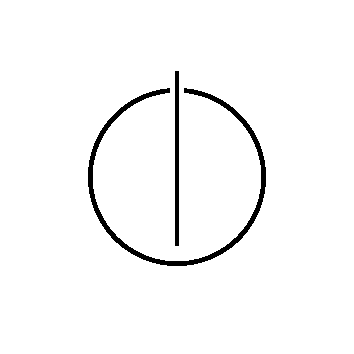
\includegraphics[width=4cm]{styles/informat.png}
  \end{figure}
  
  \end{center}
%	\clearemptydoublepage
%	
%	% The titlepage for the CAMP report document.
% Included by MAIN.TEX


%--------------------------------------------------
% The title page
%--------------------------------------------------

% correct BCOR - undo at the end !!!
\def\bcorcor{0.15cm}
\addtolength{\hoffset}{\bcorcor}

\thispagestyle{empty}

 \vspace{10mm}
\begin{center}
	       \oTUM{4cm}
	   
	   \vspace{5mm}     
	   \huge FAKULT{\"A}T F{\"U}R INFORMATIK\\ 
	   \vspace{0.5cm}
	 \large DER TECHNISCHEN UNIVERSIT{\"A}T M{\"U}NCHEN\\
        
	\end{center}
		

\vspace{10mm}
\begin{center}

   {\Large \doctype}

  \vspace{10mm}
  
  {\LARGE \title}\\
  
  
  \vspace{10mm}
  
  
  {\LARGE  \titleGer}\\
  
  
  \vspace{10mm}

    %\hfill
    \begin{tabular}{ll}
	   \Large Author:     & \Large \author \\[2mm]
	   \Large Supervisor:    & \Large Prof. Dr. Daniel Cremers \\[2mm]				
	   \Large Advisor:	& \Large Dr. J{\"u}rgen Sturm \\
	   					&	\Large (Technische Universit{\"a}t M{\"u}nchen)\\ [3mm]
	   					& \Large Adolfo Rodriguez Tsouroukdissian, PhD \\ 
	   					& \Large (PAL Robotics S.L) \\[2mm]
	   \Large Date:       & \Large April 14, 2014
	 \end{tabular}
	 
	 \vspace{5mm}
	 
	 \begin{figure}[h!]
  \centering
   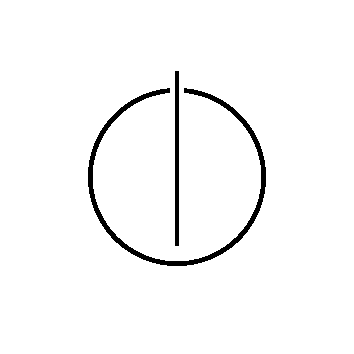
\includegraphics[width=4cm]{styles/informat.png}
  \end{figure}
   

\end{center}

% undo BCOR correction
\addtolength{\hoffset}{\bcorcor}
	
	
%	\input{components/cover_maschmeyer}
	\clearemptydoublepage
	
	% The titlepage for the CAMP report document.
% Included by MAIN.TEX


%--------------------------------------------------
% The title page
%--------------------------------------------------

% correct BCOR - undo at the end !!!
\def\bcorcor{0.15cm}
\addtolength{\hoffset}{\bcorcor}

\thispagestyle{empty}

 \vspace{10mm}
\begin{center}
	       \oTUM{4cm}
	   
	   \vspace{5mm}     
	   \huge FAKULT{\"A}T F{\"U}R INFORMATIK\\ 
	   \vspace{0.5cm}
	 \large DER TECHNISCHEN UNIVERSIT{\"A}T M{\"U}NCHEN\\
        
	\end{center}
		

\vspace{10mm}
\begin{center}

   {\Large \doctype}

  \vspace{10mm}
  
  {\LARGE \title}\\
  
  
  \vspace{10mm}
  
  
  {\LARGE  \titleGer}\\
  
  
  \vspace{10mm}

    %\hfill
    \begin{tabular}{ll}
	   \Large Author:     & \Large \author \\[2mm]
	   \Large Supervisor:    & \Large Prof. Dr. Daniel Cremers \\[2mm]				
	   \Large Advisor:	& \Large Dr. J{\"u}rgen Sturm \\
	   					&	\Large (Technische Universit{\"a}t M{\"u}nchen)\\ [3mm]
	   					& \Large Adolfo Rodriguez Tsouroukdissian, PhD \\ 
	   					& \Large (PAL Robotics S.L) \\[2mm]
	   \Large Date:       & \Large April 14, 2014
	 \end{tabular}
	 
	 \vspace{5mm}
	 
	 \begin{figure}[h!]
  \centering
   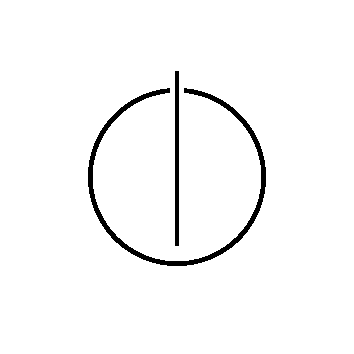
\includegraphics[width=4cm]{styles/informat.png}
  \end{figure}
   

\end{center}

% undo BCOR correction
\addtolength{\hoffset}{\bcorcor}
	
	\newpage
	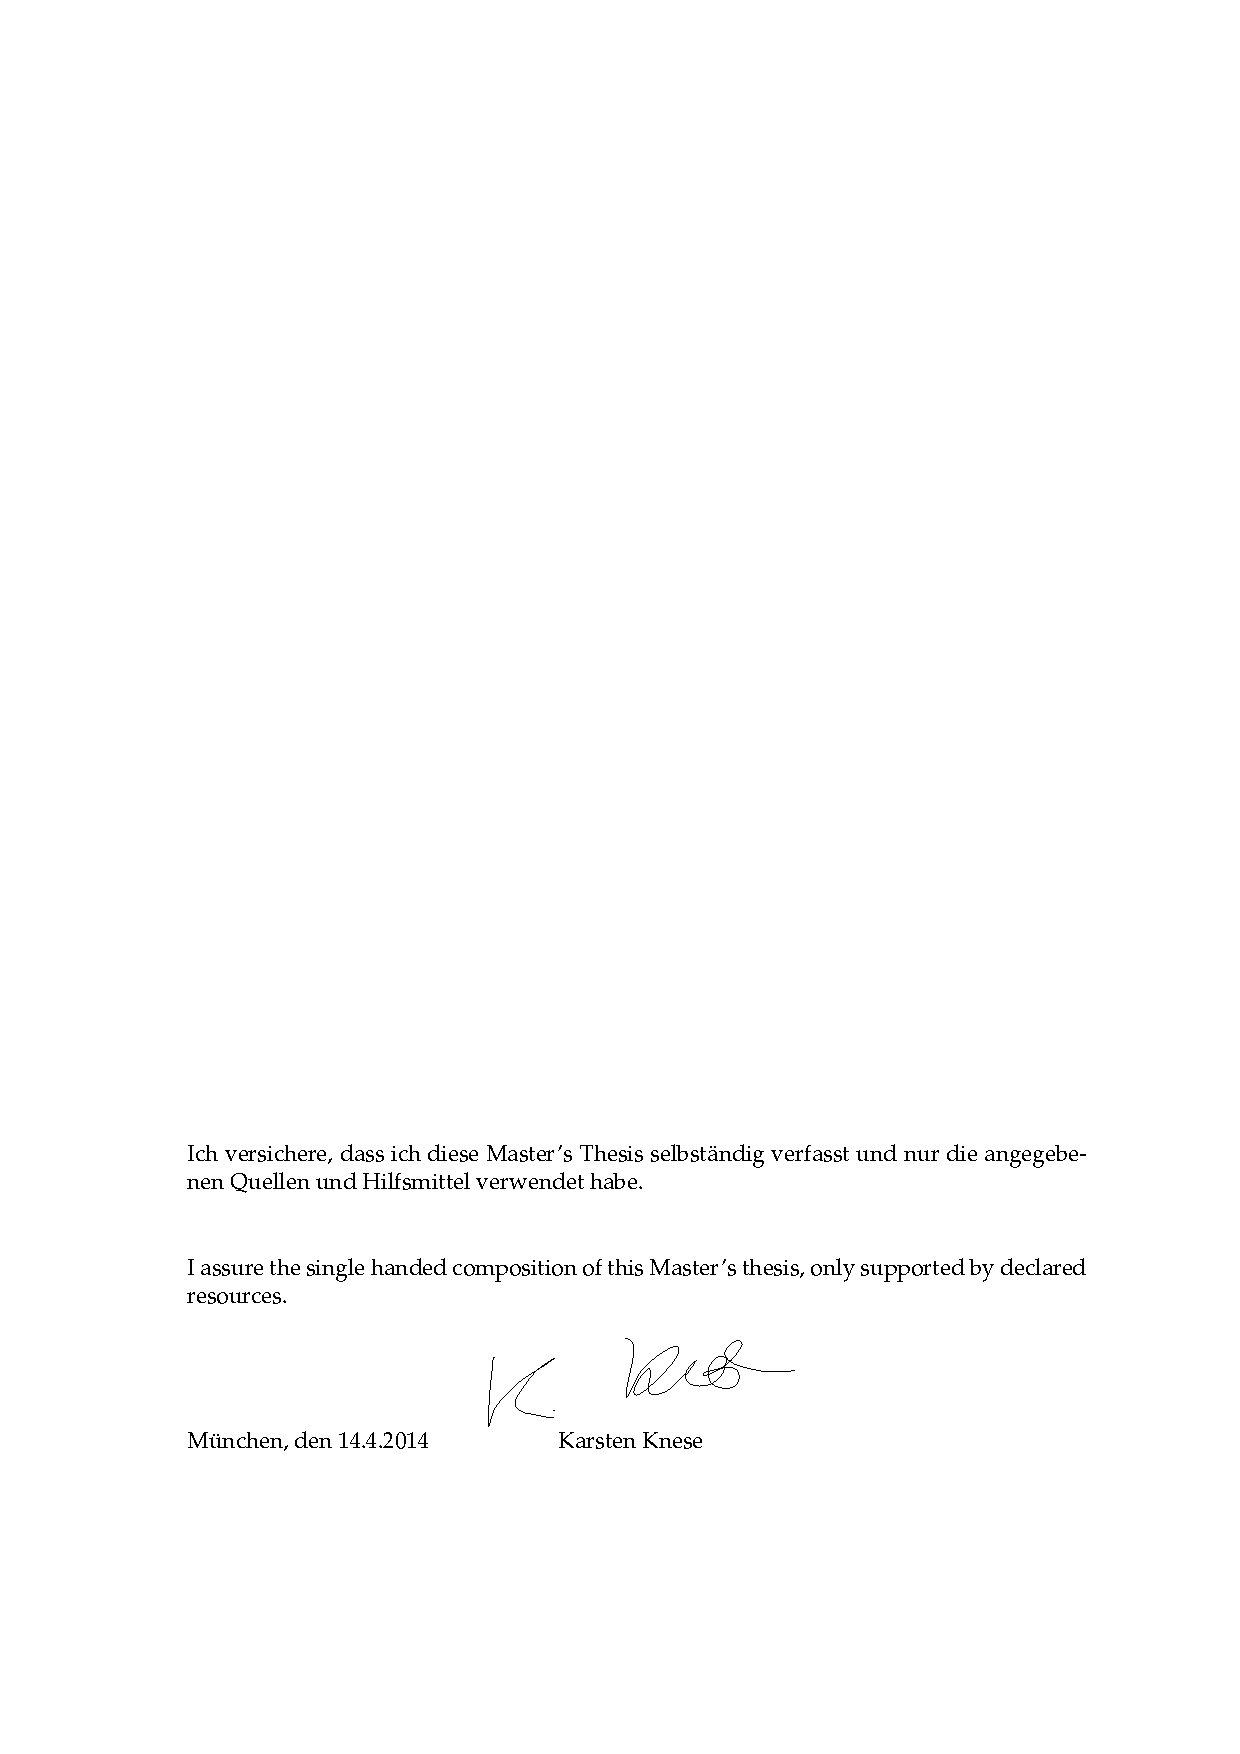
\includepdf[pages={1}]{components/disclaimer_signed.pdf}
	\newpage
	%\clearemptydoublepage

\thispagestyle{empty}
\selectlanguage{english}
	\vspace*{0.65\textheight}
	\noindent
	
Ich versichere, dass ich diese Master's Thesis selbst{\"a}ndig verfasst und nur die angegebenen Quellen und Hilfsmittel verwendet habe.

\vspace{5mm}
\noindent
I assure the single handed composition of this Master's thesis, only supported by declared resources.
	
	\vspace{15mm}
	\noindent
	M{\"u}nchen, den 14.4.2014 \hspace{2cm} \author
\selectlanguage{english}
\newpage
	
	\clearemptydoublepage
\phantomsection
\addcontentsline{toc}{chapter}{Acknowledgments}	


%\chapter*{Acknowledgements}

\vspace*{2cm}

\begin{center}
{\Large \bf Acknowledgments}
\end{center}

So here it is, my Master's thesis! Despite the fact, that my name is stated as the single author of this work, this document is written in a 'we' formulation. And this has to be taken seriously! This work could not have been realized in the way it is without the help and support of various talented minds.

To begin with, my highest appreciation and biggest 'thank you' belongs to Gennaro Raiola, for his elementary work of bringing the Stack-of-Tasks to life inside PAL Robotics. He was not only a patient colleague, but furthermore became a good friend, who made my time in Barcelona as good as it was.

I want to thank Adolfo Rodr{\'i}guez Tsouroukdissian, who mentored my work inside PAL and guided me through all arising troubles with smart ideas. Equally to J{\"u}rgen Sturm, who took not just care about all academic bureaucracy, but also gave me valuable feedback for designing this work. 

Furthermore, a big thanks goes to Hilario Tom{\'e}, who was patient and compassionated enough to reveal all necessary mathematical myths, I encountered during this work; Paul Mathieu and Bence Magyar for enlightening me with insights of C++ and ROS; Various lovely people all around the globe for cross-reading this document.

Altogether, I want to thank my colleagues at PAL Robotics, who are a great team and make working there as much fun as it could be. 

\vspace{1cm}

	%abstract english
	% Abstract for the TUM report document
% Included by MAIN.TEX


\clearemptydoublepage
\phantomsection
\addcontentsline{toc}{chapter}{Abstract}	

\vspace*{1cm}
\begin{center}
{\Large \bf Abstract}
\end{center}
\vspace{1cm}

Humanoid robots comprise a high number of redundancy, which can be used to achieve multiple goals in parallel. A hierarchy of tasks is often implemented in order to execute them simultaneously. However, this emerges a high risk of (self-)collisions, where a reactive and online collision avoidance has to be instantiated inside the hierarchy.  	

In this Master's thesis, a solution for highly dynamic (self-)collision avoidance is presented. The collision avoidance is realized as an inequality constraint inside the Stack-of-Tasks. 

Our proposed (self-)collision avoidance is implemented for the quadratic programming solver inside the Stack-of-Tasks. The alignment of linear constraints in form of a stack enables an iterative solving progress with respect to priorities given to these constraints. Hence the name, Stack-of-Tasks. The collision avoidance task is based on the closest point pair of possible collisions between two body parts. To achieve a unique solution for the closest point pair, a complete capsule decomposition for the robot model is created. The pseudo convexity of capsules reduces the number of discontinuities and leads to a smooth transition. The velocity along the unit-vector of these two points is limited by a threshold, dependent on the corresponding distance. The projection of the Jacobian towards the collision center point is reduced to zero if the inequality boundary is hit, thus disabling any movement towards the collision center. The same method can be used for self-collision avoidance as well as avoidance of external collision objects.

In order to keep the computational cost to a minimum, the dynamic graph inside the SoT is exploited in a way, that only the necessary closest point pairs are recomputed. This implies an efficient on-demand computation of the collision matrix. The self-collision is placed on a high level inside the hierarchy to ensure a constant collision check. On the same hand, the applied method allows a smooth execution of lower prioritized tasks of interest.
%
%Self-collision avoidance should always serves only as an invisible constraining task and never obviously interfere with the actual task of interest, such as positioning the manipulator. The applied method fulfills this requirement, since it is considered as inactive as long as the operation is outside a specified security distance. It only becomes active, when a violation of this security distance would happen. Therefore, we could develop further applications, such as tele-operation, visual servoing or ball grasping, in a safe manner. 
	
	% Abstract for the TUM report document
% Included by MAIN.TEX


\clearemptydoublepage
\phantomsection
\addcontentsline{toc}{chapter}{Abstract - Deutsch}	

\vspace*{1cm}
\begin{center}
{\Large \bf Abstract - Deutsch}
\end{center}
\vspace{1cm}

Humanoide Roboter besitzen eine Vielzahl von redundanten Aktuatoren, die benutzt werden k{\"o}nnen, um mehrere Aufgaben parallel auszuf{\"u}hren. Dabei ist oft eine Hierarchie zwischen diesen Aufgaben realisiert. Das gleichzeitige Ausf{\"u}hren von Zielpositionen birgt jedoch die Gefahr von (Selbst-)Kollisionen. Das erfordert eine Kollisionsvermeidung in Echtzeit innerhalb dieser Hierarchie. 	

In dieser Masterarbeit pr{\"a}sentieren wir eine vollst{\"a}ndige L{\"o}sung f{\"u}r eine hoch-dynamische (Selbst-)Kollisionsvermeidung. Diese ist realisiert als eine Ungleichheitsbedingung innerhalb des Stack-of-Tasks.

Unsere vorgeschlagene Methode zur (Selbst-)Kollisionsvermeidung ist implementiert f{\"u}r den Quadratic Program Solver innerhalb des Stack-of-Tasks. Die Anordnung der linearen Bedingungen geschieht in Form eines Stacks, was eine iterative L{\"o}sung mit Respekt zu den gegebenen Priorit{\"a}ten erlaubt. Daher der Name Stack-of-Tasks. The Kollisionsvermeidung basiert auf der Berechnung der k{\"u}rzesten Distanz zwischen zwei Kollisionsobjekten. Um eine eindeutige L{\"o}sung f{\"u}r diese Distanz zu erzielen, schlagen wir eine Darstellung des Roboterkollisionsmodells durch Kapseln vor. Die Pseudokonvenxit{\"a}t von Kapseln verringert die m{\"o}glichen Diskontinuit{\"a}ten. Die Geschwindigkeit entlang des Einheitsvektors der k{\"u}rzesten Distanz is limitiert durch einen Schwellwert. Die Projektion der Jacobianmatrix auf den Richtungsvektor wird auf Null reduziert, wenn der Grenzwert der Ungleichheit erreicht ist. Die gleiche Methode kann f{\"u}r Selbstkollisions- als auch f{\"u}r externe Kollisionsvermeidung verwendet werden.

Um die Ausf{\"u}hrungszeit minimal zu halten, wird der Dynamic Graph innerhalb des SoT aufgenutzt um nur die notwendigen k{\"u}rzesten Distanzen zu berechnen. Die Kollisionsvermeidung besitzt eine hohe Priorit{\"a}t innerhalb der Hierarchie. Gleichzeitig erlaubt unsere Methode eine reibungsfreie Ausf{\"u}hrung von niedrig priorisierten Aufgaben.

	\tableofcontents
  
  %\clearemptydoublepage

\phantomsection
\addcontentsline{toc}{chapter}{Outline of the Thesis}

\begin{center}
	\huge{Outline of the Thesis}
\end{center}




%--------------------------------------------------------------------
\section*{Part I: Introduction and Theory}

\noindent {\scshape Chapter 1: Introduction}  \vspace{1mm}

\noindent  This chapter presents an overview of the thesis and it purpose. Furthermore, it will discuss the sense of life in a very general approach.  \\

\noindent {\scshape Chapter 2: Theory}  \vspace{1mm}

\noindent  No thesis without theory.   \\

%--------------------------------------------------------------------
\section*{Part II: The Real Work}

\noindent {\scshape Chapter 3: Overview}  \vspace{1mm}

\noindent  This chapter presents the requirements for the process.

	\mainmatter
	
		% ---------------------------------------------------------------------------
		%
		%Introduction and Background Theory
		%
		% ---------------------------------------------------------------------------
		\part[Introduction and Theory]{Introduction and Theory}
		\label{part:introAndBackgroundTheory}
		
		\chapter{Motivation}
\label{chapter:introduction}
\section{Problem Statement}
Robot technology is constantly increasing as the performance of the used hardware components enable highly complex software computations. State-of-the-art robots such as REEM-C \cite{reemspec}, Asimo \cite{asimospec}, Hubo \cite{hubospec} and Atlas \cite{atlasspec} indicate that humanoid robots are capable of achieving versatile goals in appropriate time. Videos such as \href{http://www.youtube.com/watch?v=N_m56irWKeI}{this}\footnote{\url{http://www.youtube.com/watch?v=N_m56irWKeI}} expose the remarkable speed of kinematic capabilities.
\begin{figure}[h!]
  \centering
    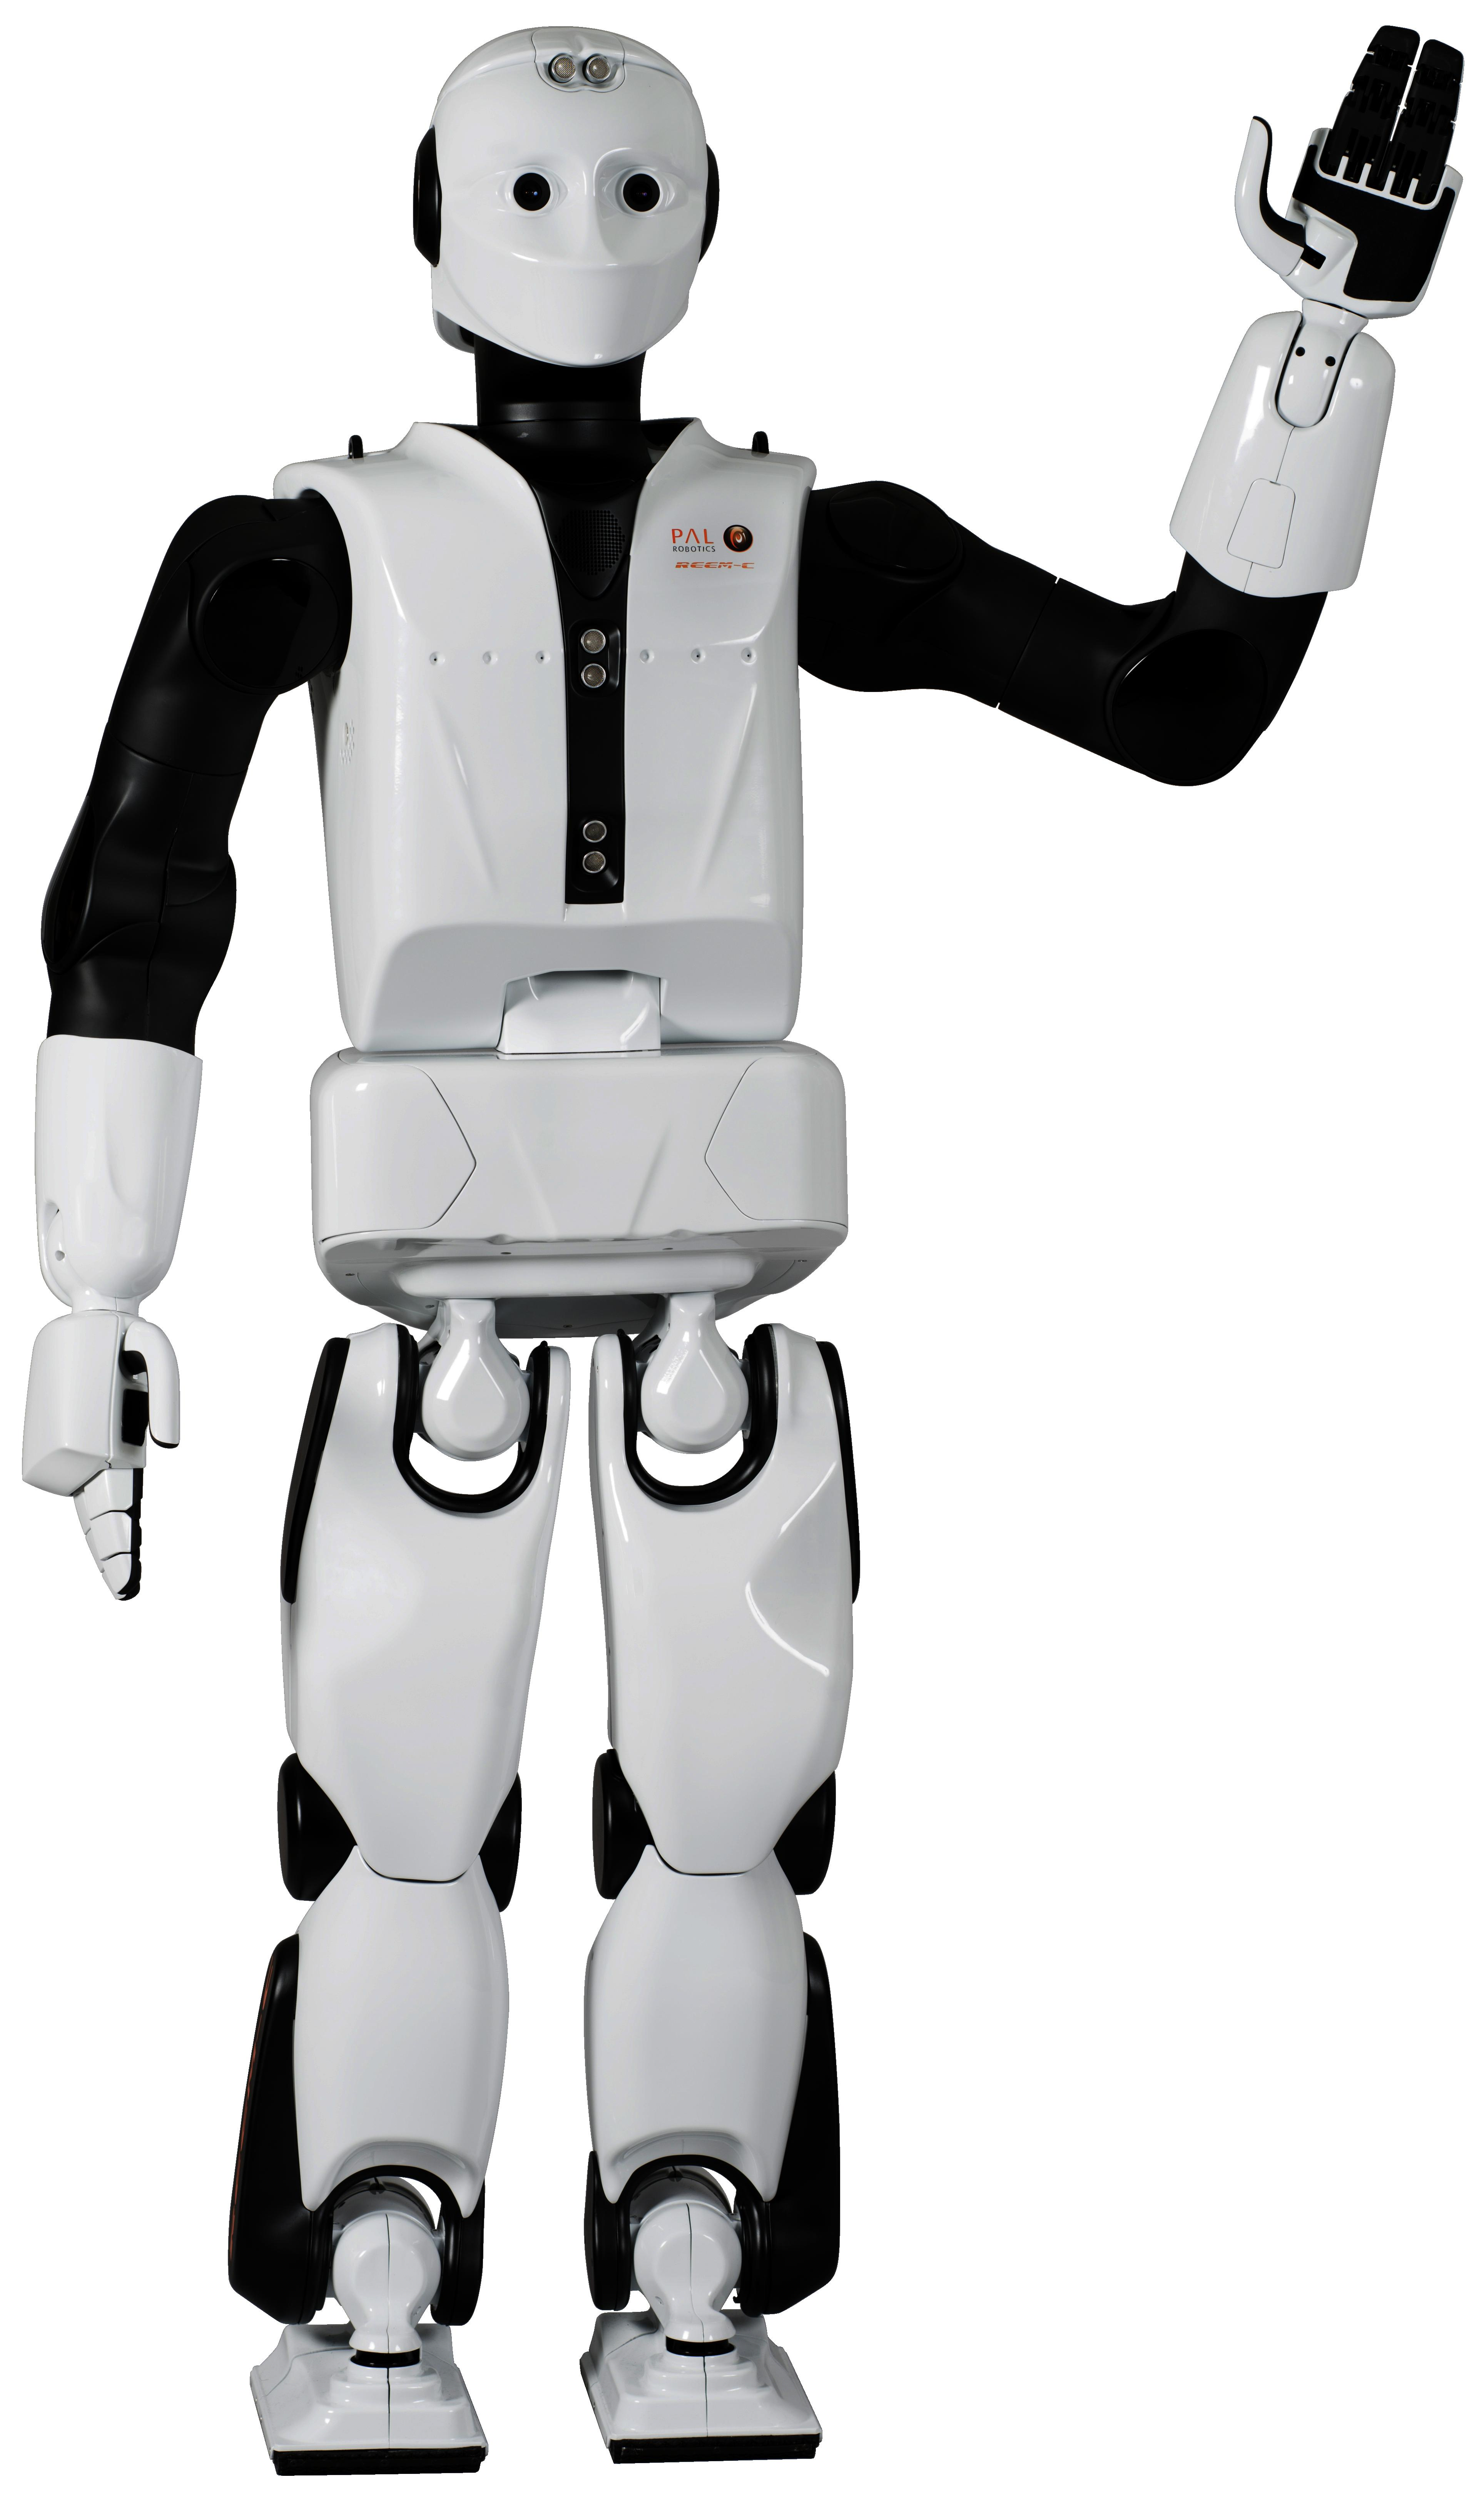
\includegraphics[width=0.18\textwidth]{../figures/reemc2.jpg}
    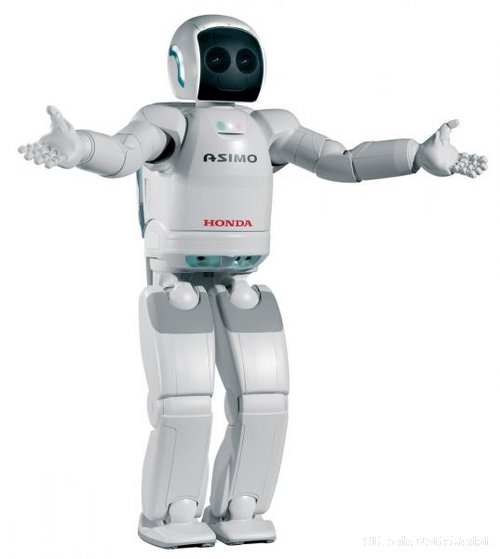
\includegraphics[width=0.23\textwidth]{../figures/asimo2.jpg}
    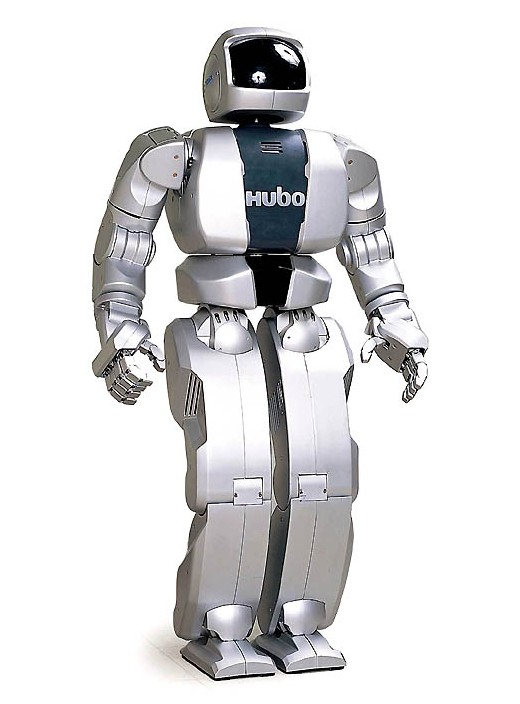
\includegraphics[width=0.23\textwidth]{../figures/hubo.jpg}
    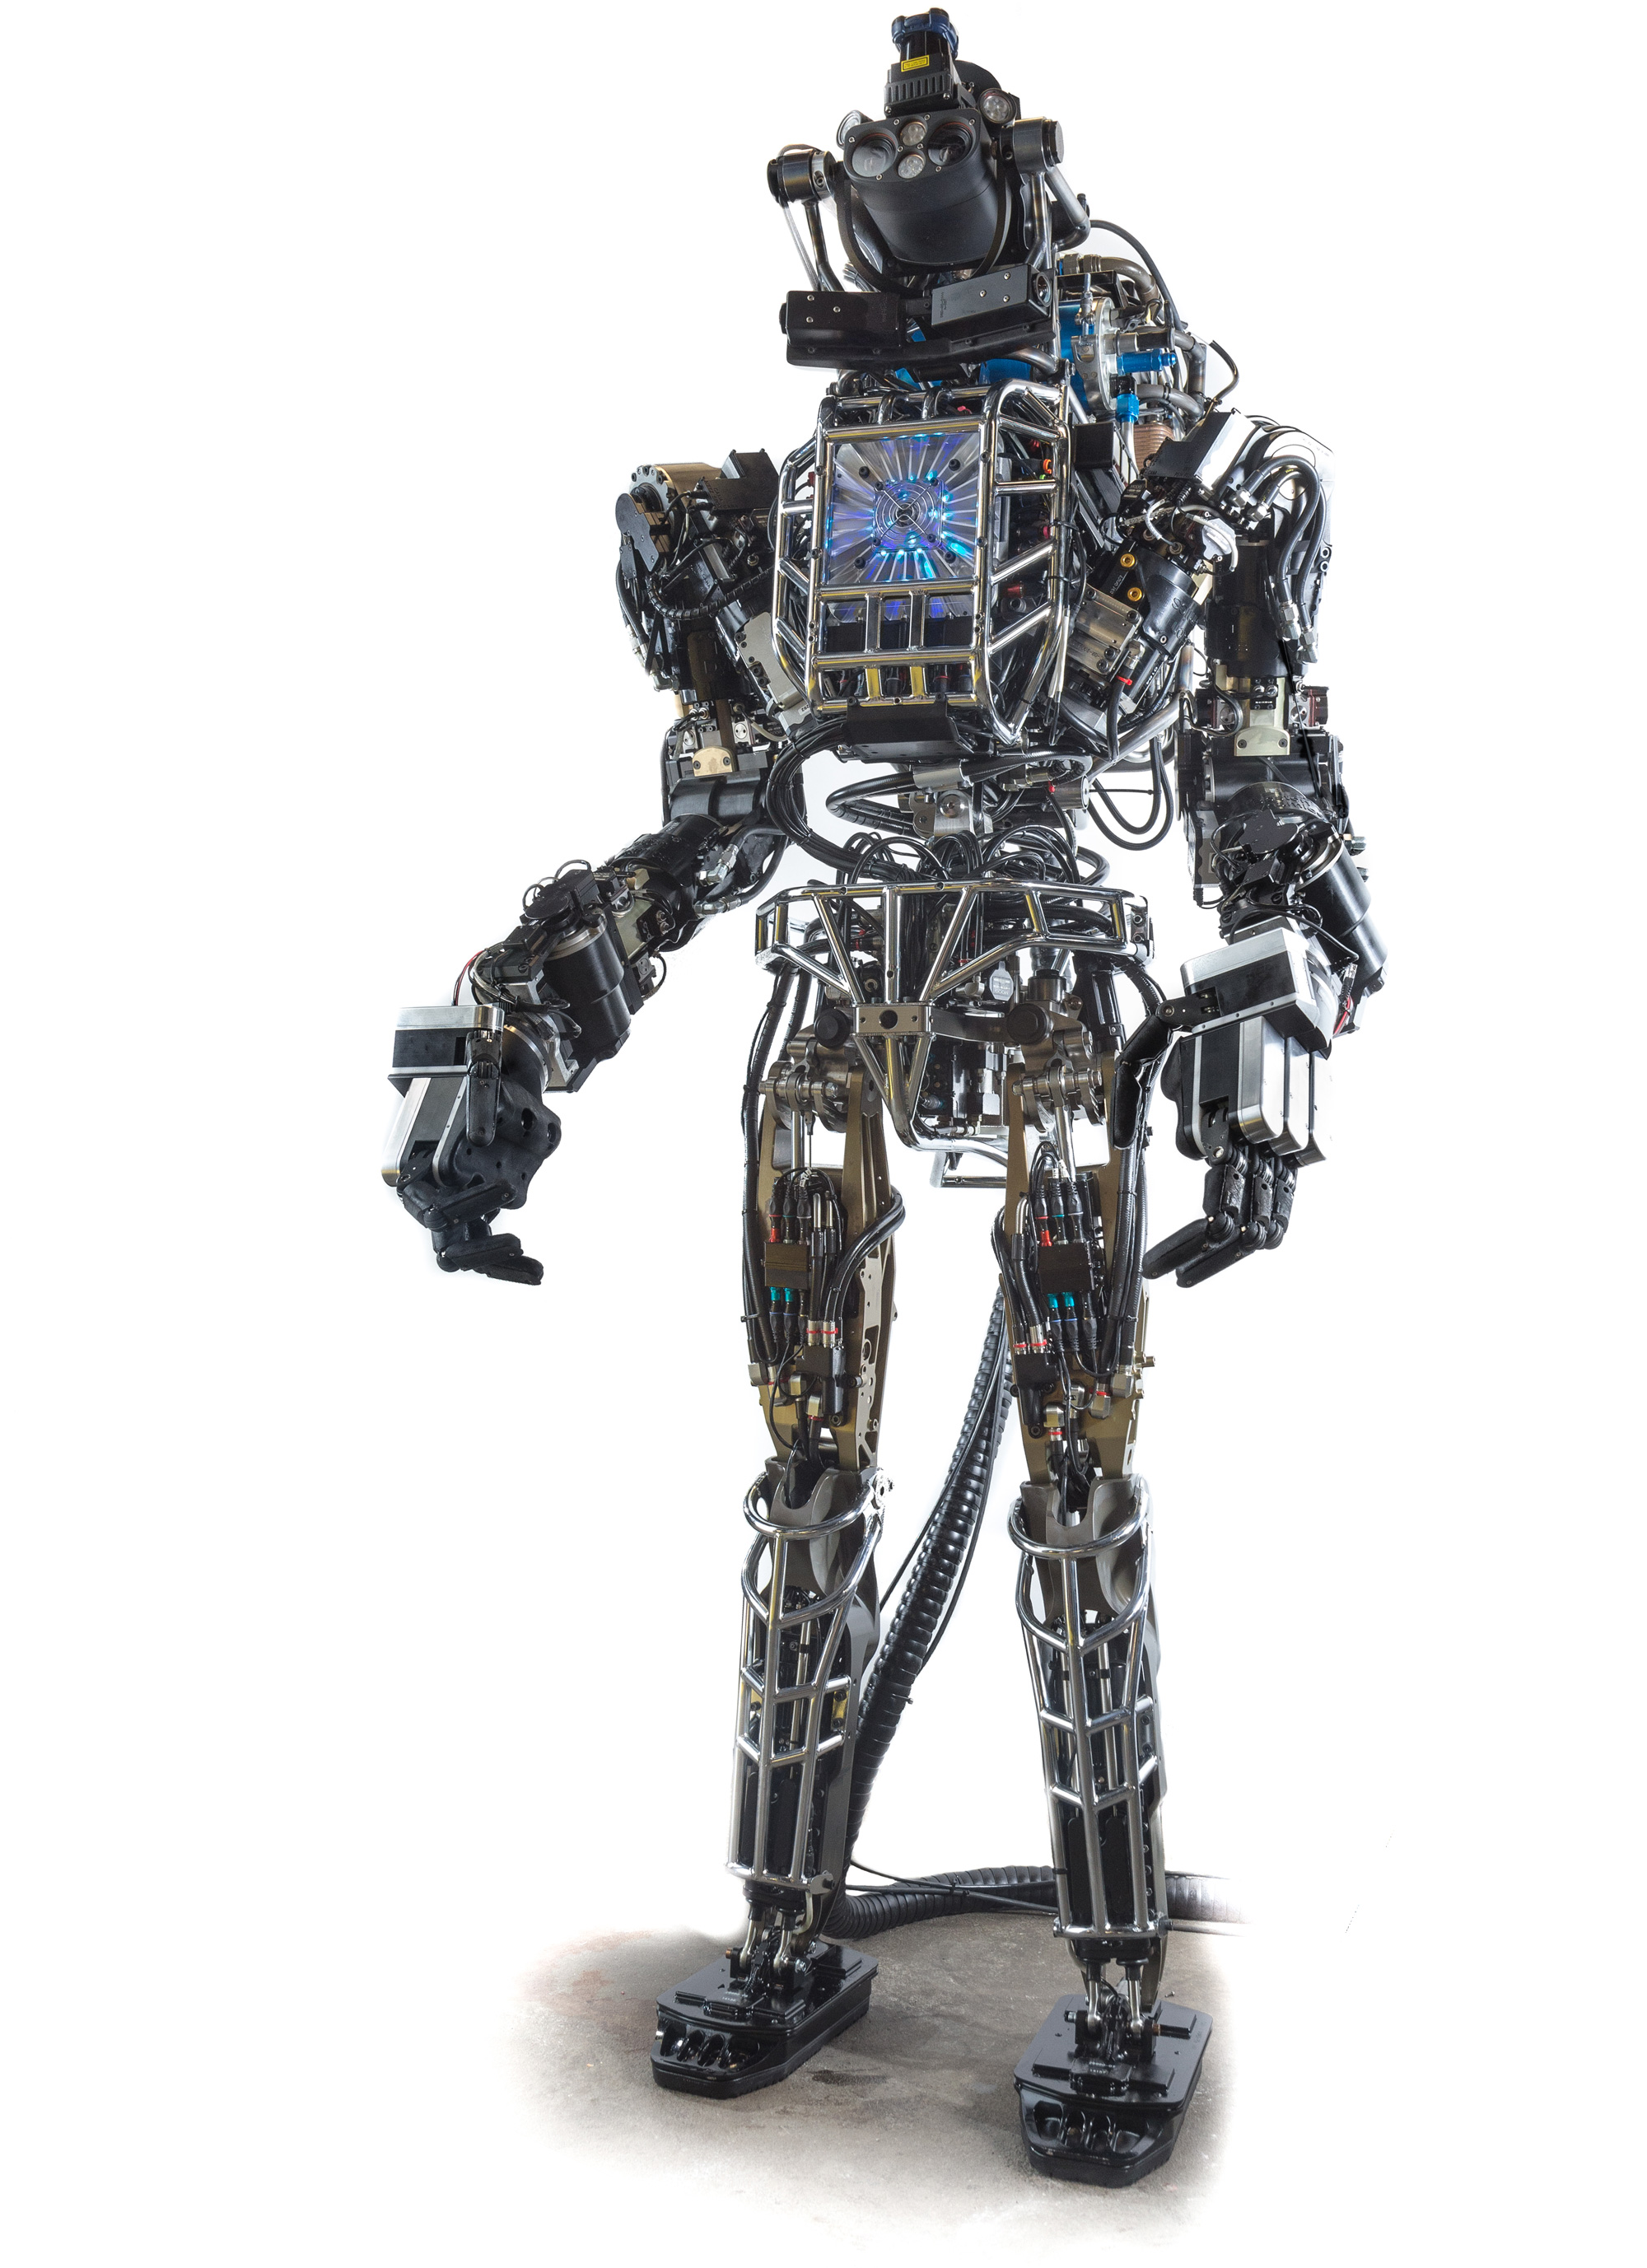
\includegraphics[width=0.23\textwidth]{../figures/atlas.jpg}
    \caption{State-of-the-art humanoid robots. From left: REEM-C, Asimo, Hubo, Atlas}
    \label{figclosestpointmesh}
\end{figure}
The dexterity and execution speed of humanoid robots thus encourage their integration into human environments. The idea of a robot accompanying a human in his daily life is becoming closer to practice. Complex tasks such as cleaning, ironing clothes or acting as a personal assistant are no longer futuristic visionary ideas, but already realizable at this time. 

What follows is the necessity of addressing safety issues, which emerge as a consequence of high execution velocities. Collisions with the robot environment as well as with the robot themselves have to be stringently avoided at all times. This becomes non-trivial especially with versatile humanoid robots, as they might easily collide with themselves, due to the redundant degrees of freedom (DOF) or the overlapping workspace of the attached manipulators (hand to hand collision). 

One way to handle collisions can be achieved by utilizing offline motion planners \cite{LaValle04planningalgorithms}. The complete scene is captured and an optimal solution without any collisions is planned. Once the trajectory is found, it is executed on the robot \cite{conf/iros/LiuDZ05}. In order to increase the speed of this planning step, especially with respect to avoiding obstacles, various optimization approaches are suggested. Rapidly-Exploring Random Trees (RRT) \cite{Lavalle98rapidly-exploringrandom} or Kinodynamic Motion Planning by Interior-Exterior Cell Exploration (KPIECE) \cite{644} are two methods, which are widely integrated in current motion planning libraries \cite{ompl}. Probabilistic Roadmaps (PRM) \cite{Kavraki96probabilisticroadmaps} are equally efficient, when the complete scene is known a priori. Probabilistic approaches \cite{Thrunprobabilisticalgorithms} are generally used to find an optimal solution. 

As the name \textit{offline} planner suggests, the trajectory planning and collision avoidance occur before the actual execution. Since the perception of the environment is still computational expensive, it is not surprising that those approaches are less efficient in dynamic environments. A fast-changing environment demands a highly reactive change of the current trajectory, still avoiding any collisions. \\
\textit{Reactive} collision avoidance algorithms try to overcome this issue. A first approach was based on repulsive forces emitted by the obstacles \cite{Khatib:86g}. Real time enabled collision avoidance based on repulsive forces have been broadly used on humanoid robots \cite{conf/humanoids/SugiuraGJG06} \cite{Xie98real-timecollision}  \cite{conf/iros/SetoKH05}. 
An enhanced development of this approach has been examined by calculating the closest point pairs between two collision objects and orient the repulsive force along the resulting directional vector \cite{conf/icra/DietrichWTAH11}. However, this implies a continuity of these calculated point pairs in order to avoid singularities and the resulting high velocities on the robot actuators \cite{escande:itro:2013}.

Since humanoid robots are highly over-actuated systems, their redundancy implies a null\-space optimization \cite{12020}, in which multiple goals can be achieved simultaneously. Within this, whole body motion control describes how to achieve a desired goal pose, utilizing all available joints. However, since multiple goal tasks can conflict with each other, priority levels are commonly used \cite{ROB:2555180}\cite{Sentis:06} and can be solved in a recursive hierarchical manner \cite{siciliano1991general}. We have therefore developed a method that ensures a collision avoidance on a high priority, but equally provides a sufficiently large nullspace to execute lower priority tasks. 
\newpage
\section{Goals of this thesis}
This work presents a complete solution for external as well as self-collision avoidance of humanoid robots. The presented implementation is based on the proposed algorithm in \cite{stasse-icra-08}. The collision avoidance is realized as an inequality constraint inside the Stack-of-Tasks (SoT) \cite{mansard:icar:09}, which serves as the base framework throughout this work. The SoT provides a highly efficient solver for hierarchical quadratic programming, which allows the execution of simultaneous goals in a whole body control manner. The algorithm in \cite{stasse-icra-08} restricts any movement along the directional vector between two closest points. In order to achieve a smooth trajectory of the closest point pair, we suggest a complete capsule decomposition as the robot's collision representation. The closest point pair is thus calculated between two capsules in order to ensure a smooth continuation in time.\\
This work is developed on two humanoid robots from PAL Robotics S.L., namely REEM-H and REEM-C. Since both robots are completely ROS based, the first goal is to integrate the SoT inside the ROS environment. 

As a summary, solutions for the following goals are presented:
\begin{itemize}\label{item:goals}
\item Integrate the SoT inside a ROS based environment to enable the execution on PAL Robotics humanoid robots
\item Assemble the robot collision model through a complete capsule decomposition to allow a smooth and continuous calculation of a closest point pair
\item Implement a collision avoidance task inside the SoT, utilizing the calculated point pair to ensure no self-collision and to enable support for external collision avoidance.
\end{itemize}

\section{Overview of this thesis}
Part \ref{part:introAndBackgroundTheory} of this work explains all the theoretical details, which are necessary for understanding the concepts implemented in this work. After this introduction, chapter \ref{chapter:soth} introduces the Stack-of-Tasks (SoT) from a theoretical point of view. We present background information about how to specify tasks based on equality and inequality constraints inside a quadratic program. Since the main objective of this thesis is the development of a collision avoidance task, we dedicate chapter \ref{chapter:collisionavoidance} to details on the implemented method. 

Implementation details and practical experiments, conducted on the robot are presented in part \ref{part:implementation}. We briefly introduce the implementation environment in chapter \ref{chapter:implenv}, where we describe ROS\_control as the main control framework, running on REEM-H and REEM-C. We further give information on how to integrate the SoT into a ROS based environment. Since the SoT comprises a complete framework, including the numerical solver, we describe the main functionalities, which are necessary for implementing a (self-)collision task. The main method, which is implemented to achieve a successful collision avoidance, has to be supplemented with additional tasks, e.g. joint limits. The instantiated tasks, which run on the robot to perform successful collision avoidance, are presented in chapter \ref{chapter:collisionavoidanceimpl}. In order to evaluate the implemented methods, various tests for all specified goals of chapter \ref{item:goals} are examined and analyzed in chapter \ref{chapter:experiments}. Finally, in chapter \ref{chapter:applications} we provide applications, which are successfully realized and give an outlook about further developments.
		\chapter{Related Work - Stack of Tasks}
\label{chapter:soth}

The Stack-of-Tasks (SoT) is an efficient framework for hierarchical quadratic programming (QP) \cite{kanoun:itro:11}. It implements a General Inverse Kinematics (GIK), which was firstly presented in \cite{nakamura}. A task denotes an abstract desired goal value, which can be achieved by controlling an ordinary differential equation \cite{ROB:2555180}. Tasks can be, among others, a desired pose of a manipulator, a gaze task describing a point in a 2-dimensional plane or a range of allowed joint values. Whole body motion control implies a high number of DoF and with it a lot of redundancy. Thus it becomes obvious that multiple instances of those tasks can be regulated simultaneously \cite{Liegeois1977}. A widely common approach is to install a hierarchy of tasks, solving them recursively in respect of the precedent nullspace \cite{siciliano1991general}.  \\
\\
Generally, the SoT provides two main functionalities. Firstly, it incorporates a QP solver in a hierarchy preserving manner \cite{mansard-tro-09}. Hereby, a novel and highly computationally efficient matrix decomposition was introduced, which yields a remarkable improvement in terms of computation speed \cite{escande-ijrr-sub12}. \cite{escande-icra-10} refers to this specific development as Hierarchical Complete Orthogonal Decomposition (HCOD), which is adopted throughout this work when the emphasis is attached to the solver itself rather than the overall framework.\\
\\
Secondly, the SoT describes a software framework, which implements an intelligent way of establishing a dynamic hierarchy by activating and deactivating task constraints on runtime. In the remainder of this chapter, the focus lies on the theoretical aspect of numerically solving the hierarchy of tasks. Complementary, the implementation of the software framework takes place in the second part of this work in chapter \ref{chapter:implenv}.

\section{Prerequisites}
The SoT is the base line of this work. In order to ease the understanding of the concepts presented in the following, a few requisites are recalled. The inverse kinematic solver mainly works with a least-square pseudo inverse approach, which can be formulated as a constrained quadratic programming problem. Finally, the SoT implements an inverse kinematics control scheme to run in real time on the robot.
\subsection{Least Square}
Least Squares is a way to optimize problems to its best. It applies always to overdetermined problems, where there exists no unique solution. This is the case, when there are more linearly independent equations than unknowns. 
\begin{equation}\label{eqn:leastsquare}
Ax = b \quad \text{with } A \in \mathbb{R}^{m \times n}, m < n
\end{equation}
Since $A$ is strictly skinny matrix, there is no direct inverse in order to analytically solve this equation system. However, we can optimize this system to its best, meaning we minimize the resulting error, when we take all equations into consideration. Equation \ref{eqn:leastsquare} thus turns into
\begin{equation}\label{leastsquareerror}
r = Ax -b
\end{equation}
The optimization is formulated as follows:
\begin{equation}
x^* =  \underset{x}{\text{arg min}} \left\| Ax - b \right \|
\end{equation}
The solution can be found by minimizing the squared residual. Minimizing means computing a solution for the first derivative set to zero.
\begin{eqnarray}
\left\| r \right\|^2 &=& xA^TAx - 2b^TAx + b^Tb  \label{eqn:leastsquarevebose}\\
\nabla_x \left\| r \right\|^2 &=& 2 A^TAx - 2A^Tb = 0
\end{eqnarray}
This further yields to the solution of the normal equation
\begin{eqnarray}
A^TAx &=& A^Tb \\
x &=& A^T(A^TA)^{-1} b \\ \label{eqn:pseudoinverse}
x &=& A^+b
\end{eqnarray}
where equation \ref{eqn:pseudoinverse} describes the famous Moore-Penrose pseudo inverse.

\subsection{Quadratic Programming}
Quadratic Programming handles optimization problems with linear equality or inequality constraints. Hence the name, the primal objective function to optimize is a quadratic function. The general problem statement can be formulated as follows:
\begin{eqnarray}\label{eqn:qp}
\frac{1}{2}x^TQx + c^Tx + r_o \\
\text{subject to } Dx = e \quad \in \mathcal{E} \\
\text{subject to } Dx \leq e \quad\in \mathcal{I} 
\end{eqnarray}
Since the objective function describe a quadratic function, a least square formulation can be easily transformed into a QP. 
From the equation in \ref{eqn:leastsquarevebose}, it can be easily seen that this equation has the same shape as equation \ref{eqn:qp}.

We can solve general QP problems by applying Lagrange multiplier for each constraints. We formulate the Lagrangian equation by multiplying each constraint and optimize for $x$ and $\lambda$.
\begin{equation}\label{eqn:lagrangian}
\mathcal{L}(x,\lambda) = \frac{1}{2}x^TQx + c^Tx + r_o + \lambda^T (Dx-e)
\end{equation}
The Karush-Kuhn-Tucker conditions \cite{kuhn50nonlinear} for this are given as follows
\begin{eqnarray}
\nabla \mathcal{L}(x, \lambda) &=& 0 \\
d_i^Tx &=& e_i \quad \in \mathcal{E} \\
d_i^Tx &\geq & e_i \quad \in \mathcal{I} \\
\lambda &\geq & 0 \quad \in \mathcal{I} \\ \label{eqn:kktineq1} 
\lambda (d_i^Tx-e_i) &=& 0 \quad \in \mathcal{I} \label{eqn:kktineq2} 
\end{eqnarray}
When we look closer at the last two conditions \ref{eqn:kktineq1} and \ref{eqn:kktineq2}, we can see that all active inequality constraints have to be satisfied. Condition \ref{eqn:kktineq1} emphasizes that only constraints are valid and thus optimized, where their according $\lambda$ is positive. Conditions with positive Lagrange multipliers are not considered to contribute to an optimal solution. Moreover, inequalities are called satisfied, when the optimal solution lies directly on the border. Thus, an inequality turns into an equality constraint (condition \ref{eqn:kktineq2}) and can be solved in a least square sense. 

Considering those two conditions, we always have to find the optimal set of inequality constraints, which are active and thus can be solved in a equality like behavior. Prominent approaches are Simplex algorithms \cite{murty1983linear} and Active Set Search\cite{GVK502988711} methods. The latter will be explained in more detail in the remainder of this chapter. 


\subsection{Inverse Kinematics Control Scheme}\label{subsec:ik}
GIK can be solved with a geometrical approach\cite{c1983geometric} just to a certain extend \cite{citeulike:1090825}. When the number of actuated joints increases, in particular in redundant manipulators, an numerical approach for solving the inverse kinematics problem is widely chosen \cite{springer}. The differential equation for the inverse kinematics describes a linear mapping between cartesian space and operational space
\begin{equation}
\vec{\dot{x}} = \vec{J}\vec{\dot{q}}
\end{equation}
where $\vec{\dot{x}}$ denotes a velocity in cartesian space, whereas $\vec{\dot{q}}$ defines the robot control input vector. The Jacobian matrix $\vec{J}$ describes the linear mapping function between the two spaces. From the above formulation, we can see the similarity to the least squares equations. Thus, since a redundant manipulator describes an overdetermined system, it makes sense to solve this optimization problem with a pseudo-inverse approach.
\begin{equation} \label{eqn:inverseIK}
\vec{\dot{q}} = \vec{J}^+\vec{\dot{x}}
\end{equation}
Redundant manipulator implies a set of possible solutions, since the system is overdetermined and thus comprises unused DoF. Those unused DoF can be used to cascade secondary objectives without violating the first constraint \cite{12020}. In order to achieve this, we can freely multiply any arbitrary vector $\vec{q_1}$ with the according projection $\vec{P_0}$ into the nullspace of the primal objective function. Therefore, we extend equation \ref{eqn:inverseIK} to
\begin{equation} \label{eqn:inverseIKnullspace}
\vec{\dot{q}} = \vec{J}_0^+\vec{\dot{x}_0} + \vec{P}_0\vec{\dot{q}}_1 
\end{equation}
where $\vec{P}$ is defined as $\vec{I} - \vec{J}^+\vec{J}$.

This formulation can be included into a real time constrained control scheme. The partial velocities, solved with the above method, are integrated over time and the resulting joint positions $\vec{q}$ are set on the respective motors. The control scheme can be formulated as follows:
\begin{equation}
\vec{q}(t_{k+1}) = \vec{q}(t_{k}) + [ \vec{J}(t_{k+1})^+\vec{\dot{x}}(t_{k+1}) + \vec{P}\vec{\dot{q}}(t_{k+1}) ] \Delta t
\end{equation}
However, since the control scheme is mainly driven by a forward control design, it makes sense to put this control scheme in dependency of a desired cartesian position $\vec{x_d}$ and regulate the resulting error between actual solution and desired position.
We formulate the error equation by incorporating the desired values
\begin{equation}\label{eqn:ikfirstorder}
\vec{\dot{e}} =  \vec{\dot{x}}_d - \vec{\dot{x}} =  \vec{\dot{x}}_d - \vec{J}\vec{\dot{q}}
\end{equation}
When we look in particular at equation \ref{eqn:ikfirstorder}, we can see a first-order differential equation. The solution as written in equation \ref{eqn:inverseIK} thus becomes
\begin{eqnarray}
\vec{\dot{q}} &=& \vec{J}^+\vec{\dot{e}} \\
			   &=& \vec{J}^+(\vec{\dot{x}}_d - \vec{\dot{x}})
\end{eqnarray}
Additionally, to complement the control law, a proportional constant $K$ is introduced as a gain parameter to optimize the convergence speed. The overall controller can be illustrated in the following diagram (figure \ref{fig:ikcontrolloop}).
\begin{figure}[h!]
  \centering
    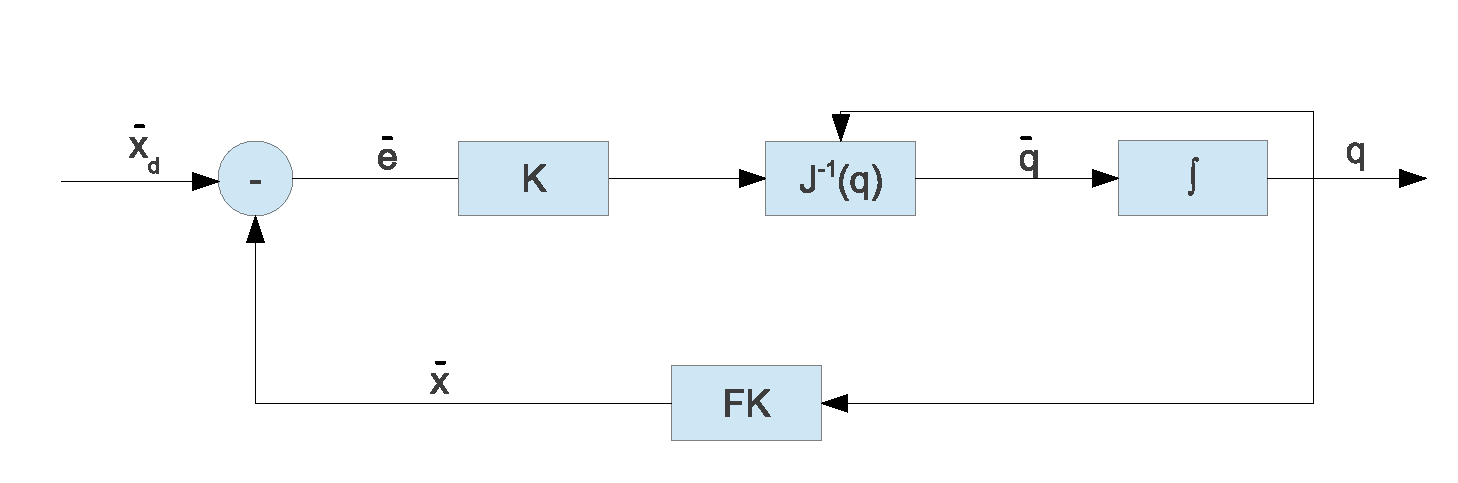
\includegraphics[width=0.8\textwidth]{../figures/ikcontrolloop.eps}
    \caption{Illustration of the Inverse Kinematics control scheme. The error is computed via the desired position $x_d$ and the current velocity provided by the Forward Kinematics $FK$.}
    \label{fig:ikcontrolloop}
\end{figure}
\section{Hierarchical Inverse Kinematics}
Current state of the art humanoid robots possess around 30-40 DoF. This allows an execution of multiple tasks in parallel. We start our examination by firstly looking at one task. When we want to control any actuated end-effector, we consume 6 DoF in $SE(3)$ Lie group \cite{LIE} for a full pose positioning. A simple manipulating task can be formulated based on a task space value $\vec{\dot{e}}$, with an unknown joint vector $\vec{\dot{q}}$ and the translating Jacobian $\vec{J}= \frac{\partial e}{\partial q}$.
\begin{equation}\label{eqn:ikcontrol}
\vec{\dot{e}} = \vec{J}\vec{\dot{q}}
\end{equation}
where $\vec{\dot{q}}$ describe the solution vector in joint velocity space, which will serve as the input of the robot.
The GIK formulation in equation \ref{eqn:ikcontrol} can be solved in a least square approach, solving the following QP to its best:
\begin{equation}\label{eqn:ikleastsquare}
\vec{\dot{q}^*} =  \underset{\dot{q}}{\text{arg min}} \left\| \vec{J}\vec{\dot{q}} - \vec{\dot{e}^*} \right \|
\end{equation}
The above QP formulation is broadly used for inverse kinematics \cite{Whitney72a}\cite{Chiaverini94reviewof} or inverse dynamics \cite{khatib-1987a}. For the remainder of this chapter, we consider a general least square approach and rename equation \ref{eqn:ikleastsquare} into
\begin{equation}\label{eqn:ikleastsquaresol}
x^* =  \underset{x}{\text{arg min}} \left\| Ax - b \right \|
\end{equation}
The solution for this optimization problem can be found by utilizing the pseudo-inverse approach \cite{journals/jirs/Siciliano90}, which yields to
\begin{equation}\label{eqn:ikleastsquaresolinv}
x^* = A^+ b \quad \text{with }A^+ = A^T(AA^T)^{-1}
\end{equation}
where $A^+$ denotes the Moore-Penrose pseudo-inverse \cite{ben2003generalized}. Considering a set of constraints, \ref{eqn:ikleastsquaresol} can be enhanced by a nullspace projection \cite{Liegeois1977} to obtain a generic solution.
\begin{equation}\label{eqn:ikleastsquarenullspace}
x^* = A^+ b  + Px_p
\end{equation}
where $P$ denotes the projection of an arbitrary vector $x_p$ into the nullspace of $A_1$. 
However, since we have a high number of redundant joints, we can execute multiple tasks in parallel. Thus, a task can be positioning an arm end-effector, keeping the vision system orientated towards a fixed point in 3-dimensional space or use both legs for walking. On the other hand, multiple tasks might not be feasible, since they either share common parts of the kinematic chain (e.g. torso links between the left and right arm) or interfere with each other. The idea is to implement a hierarchy of tasks, where the highest priority task will be solved to its best in a least square approach, whereas lower prioritized tasks are solved inside the of each respective precedent nullspace.

Equation \ref{eqn:ikleastsquarenullspace} allows us to include a secondary constraint into the QP, which does not violate the primal objective function. Considering now two tasks, we can setup a simple hierarchy based on that nullspace projection. Let $A_1,b_1$ be the primal objective and $A_2,b_2$ a secondary task, we can formulate the following hierarchical QP, substituting equation \ref{eqn:ikleastsquarenullspace} into \ref{eqn:ikleastsquaresol}:
\begin{eqnarray}
x_2^* =  \underset{x_2}{\text{arg min}} & \left\| A_2x_2 - b_2 \right \| \notag \\
& \left\| A_2(A_1^+b_1+P_1x_2) - b_2 \right \| \notag \\
& \left\| A_2P_1x_2 - (b_2 - A_2A_1^+b_1) \right \|
\end{eqnarray}
The generic solution for this QP, can be equally as in equation \ref{eqn:ikleastsquarenullspace} found with the pseudo-inverse:
\begin{equation}\label{eqn:ikleastsquarenullspaceexample}
x_2^* = (A_2P_1)^+ (b_2 - A_2A_1^+b_1)  + P_2x_3
\end{equation}
This implies that a solution for lower stacked tasks can only be found if there exists a nullspace of a precedent task. If the above task consumes all DoF, lower placed tasks can not be considered any further.

The above equation \ref{eqn:ikleastsquarenullspaceexample} is recursively formulated in \cite{siciliano1991general} for $n$ hierarchically stacked tasks.
\begin{equation}\label{eqn:ikleastsquarerecursive}
x^*_n = \sum_{k=1}^n (A_kP_{k-1})^+ (b_k - A_{k}A_{k-1}^+b_{k-1}) + P_nx_{n+1}
\end{equation}

\section{Inequality Constraints}
The above presented hierarchy describes a equality constrained Quadratic Program (eQP). This enables a simultaneous execution of multiple tasks with equality constraints, such as positioning tasks. However, in order to implement safety mechanism, no hard constraints but solution spaces are necessary, which immediately demand for inequality constraints. Safety mechanisms can be such as an active elbow-field, keeping the elbow above a certain threshold, balancing the center of mass (CoM) inside a polygon or avoiding collision with obstacles, as it is the topic of this work.

We can formulate an inequality Quadratic Program (iQP) in a classical manner:
\begin{eqnarray}
x^* =  \underset{x}{\text{arg min}} \left\| Ax - b \right \| \\
\text{subject to } Cx < d
\end{eqnarray} 
\newpage
These kind of iQP are often formulated by introducing a slack variable $w$, which indicates the level of violation \cite{kanoun:inria-00390581}. 
\begin{eqnarray} \label{eqn:ikineq}
x^*, w^* =  \underset{x,w}{\text{arg min}} \left\| w \right \| \\
\text{subject to } Cx < d + w
\end{eqnarray} 

Let us assume that $Cx <d$ fulfills all the KKT \cite{kuhn50nonlinear} conditions. We can then denote this an optimal solution set and easily solve this iQP as if it were an eQP. This means, that in an optimal set of inequalities, the solution satisfies all active constraints \cite{escande-icra-10}.

The main idea of solving such an iQP is finding the set of constraints, which form the optimal set. Those algorithms are mainly referred as Active Set Search \cite{GVK502988711} and often used to solve inequality constraint QPs. The algorithms starts with an initial guess $\vec{x}_0$ and working set $\vec{W}$ filled with activated constraints. The first step is to solve the iQP like an eQP and find the KKT optimal conditions $\vec{x}_{t=1}, \vec{\lambda}_{t=1}$. When one or many Lagrange multiplier are negative, the currently active set is not optimal, which means there are unnecessary constraints. The negative constraint $\lambda_k$ is dismissed and the algorithm starts over again with $\vec{x}_0$ and $\{ \vec{W} \setminus \lambda_k \}$ in order to solve $\vec{x}_{t=2}, \vec{\lambda}_{t=2}$. 

Once a solution is found, where $\vec{\lambda}$ is strictly positive, we perform a search step. This is by best practice performed in the direction of $\vec{v} = \vec{x}_1-\vec{x}_2$. 
\begin{equation*}
\vec{x^*_1} = \vec{x_1}+ p\vec{v} \quad \text{with } p \in [0;1]
\end{equation*}
We have to prove the new step for feasibility. We again solve the QP and activate all constraints, which are violated on the update step. The algorithm converges when all constraints are feasible and contain non-negative Lagrange multiplier.

We can see that the recursive formulation in equation \ref{eqn:ikleastsquarerecursive} is not applicable towards inequality constraints. The problem is that we can not easily find a nullspace projector $P$, as this can be a $n$-dimensional semi-infinite space. \cite{kanoun:itro:11} presents a hierarchical preserving way to solve inequality constraints in the form of equation \ref{eqn:ikineq}. Let us consider a primal objective with two inequality constraints, which are aligned in hierarchical manner.
\begin{eqnarray} \label{eqn:ikineqrecur}
\underset{x_2,w_2}{\text{arg min}} \left\| w_2 \right \| \\
\text{subject to } A_1 x < b_1 + w_1^* \\
\text{subject to } A_2 x < b_2 + w_2
\end{eqnarray}
The above formulation shows the solution approach of recursively concatenated iQP. The first inequality in \ref{eqn:ikineqrecur} provides a valid solution $x$ with respect to the least square solution of the primal objective function. With this, it is secured that the solution of $x_1$ does not change the solution in $x$. This behavior can be concatenated recursively.
\newpage
Recomputing the eQP constantly for finding the optimal active set is computational expensive \cite{escande-icra-10}. It is mainly expensive, because activating and deactivating constraints forces the recomputation of the complete stack. Furthermore, each constraint is solved on its according level and all levels beneath it. When the stack contains $n$ levels, then in particular the highest level is solved $n$ times. This is not feasible in terms of whole body motion control, as it would probably exceed all real time update cycles on a humanoid robot. The HCOD introduces an efficient matrix decomposition based on an existing Complete Orthogonal Decomposition (COD). The improvements exploits a methods, which depends only on the amount of DoF and not on the constraints. In essence, the HCOD uses a intelligent way to improve the computation speed of the Active Set Search. Furthermore, HCOD implies ways to solve the complete stack in one cycle, without recursively backtrack all beneath placed stacks. The results of HCOD exceed existing solutions by an order of magnitude in computation time. This allows a powerful setup of tasks to be executed in parallel on low powered computers. The mathematical insights of this are verbosely given in \cite{escande-ijrr-sub12} and exceed the scope of this thesis.
     	\chapter{Collision Avoidance}
\label{chapter:collisionavoidance}
In the following chapter, we introduce our proposed method for collision avoidance. We implemented an inequality task inside the SoT, which is placed as a high priority task. This task handles all collisions, but still restricts the execution of lower priority tasks as little as possible. The collision avoidance task, introduced in the following, is based on three major concepts. 
\begin{enumerate}
\item Closest point pair calculation between two collision objects
\item Damping the velocity along the normal vector, spanning from the closest point pair
\item Calculating the Jacobian for every closest point
\end{enumerate}
\section{Closest Point Calculation}\label{sec:closestpoints}
Closest point pairs are used in various algorithms for collision avoidance \cite{conf/icra/DietrichWTAH11}\cite{Kanehiro-RSS08}. Hereby, a Gilbert-Johnson-Keerthi (GJK) approach is frequently used to compute the proximity and closest points for collision detection \cite{VandenBergen:1999:FRG:334709.334711}. It is easy to understand, that preventing the closest points of two colliding objects is sufficient enough for avoiding the complete object to collide. However, this is constrained with the condition, that there is always one unique pair of closest points \cite{conf/humanoids/EscandeMK07}. 
\clearpage
\subsection{Collision Geometry - Mesh}
Most common robots come along with a description of their collision geometry. In order to make the collision geometry as accurate as possible, polygon meshes are widely used to represent the geometry of the robot. The interested reader is referred to \cite{Tobler_amesh} for more information.

Although the calculation between two meshes might fulfill the requirement of having a unique point pair between two collision objects, severe discontinuities occur inside a two dimensional space. Depending on the alignment of the vertices inside the mesh, the closest points can jump in $X$ as well as $Y$ direction, when two meshes appear to be coplanar to each other. In this case, there is ambiguity in the placement of the two points. Figure \ref{figclosestpointmesh} illustrates this behavior. The discontinuities shown here are linearly propagated to the velocity of the moving body part, which finally results in a heavy jump of velocity.\\
The discontinuities occur quite frequently in two aspects. The points can vary inside one pair of vertices as illustrated in figure \ref{figclosestpointmesh}. Additionally, depending on the shape of the mesh, multiple vertices can be projected towards the same pose, respectively a high number of normal vectors of each vertices (see figure \ref{figmeshambiguity}). This makes a closest point calculation for meshes infeasible.  

\begin{figure}[h!]
  \centering
    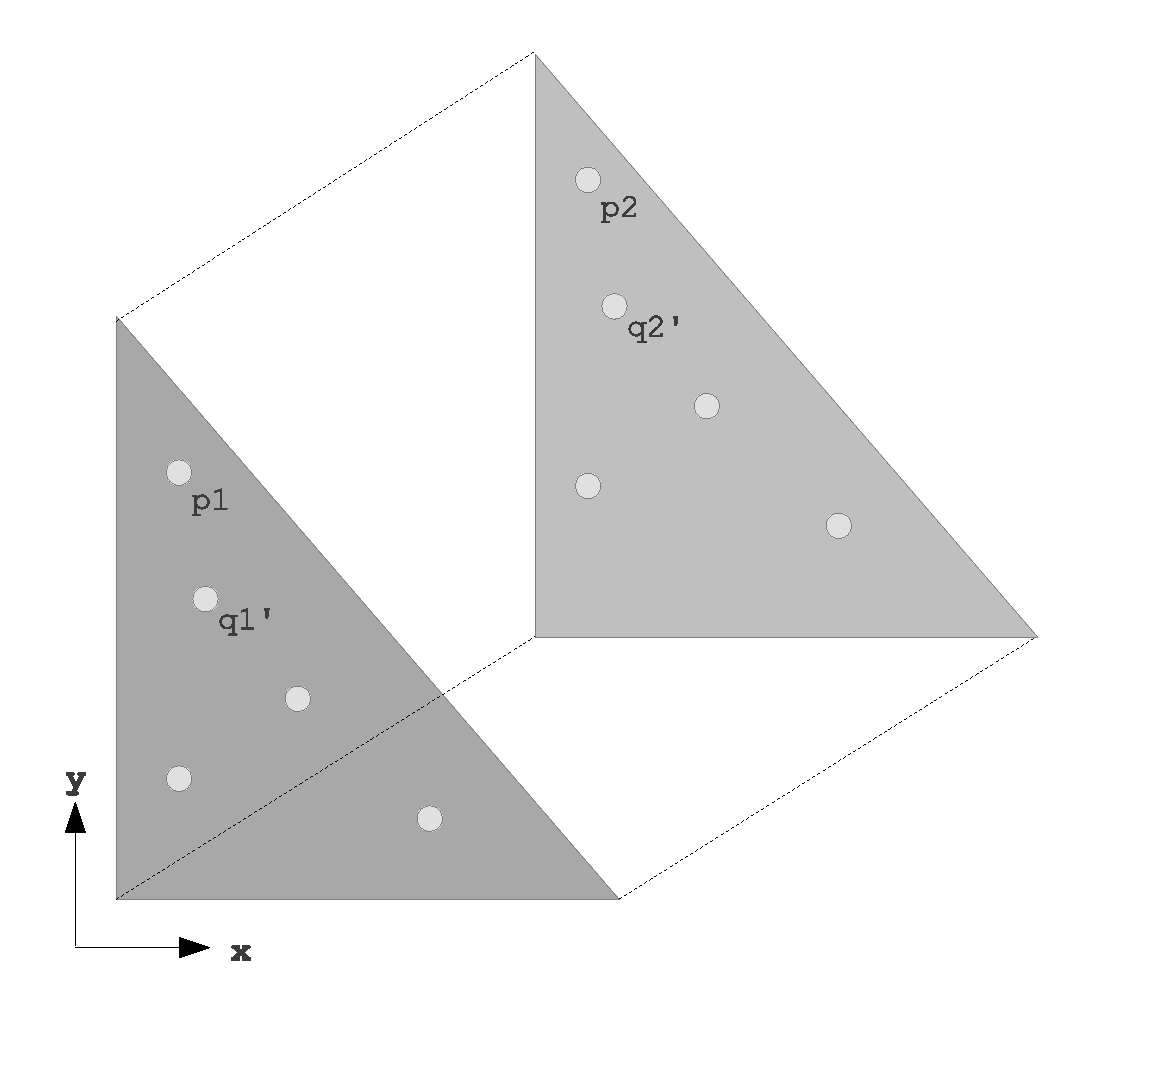
\includegraphics[width=0.6\textwidth]{../figures/closestpointmesh.eps}
    \caption{Discontinuity of closest point calculation for two vertices inside meshes. Parallelism of two vertices produces an ambiguity of the point pair. As depicted here, multiple solutions exists such as $p1$, $p2$ as well as $p1'$, $q2'$.}
    \label{figclosestpointmesh}
\end{figure}

\begin{figure}[h!]
  \centering
    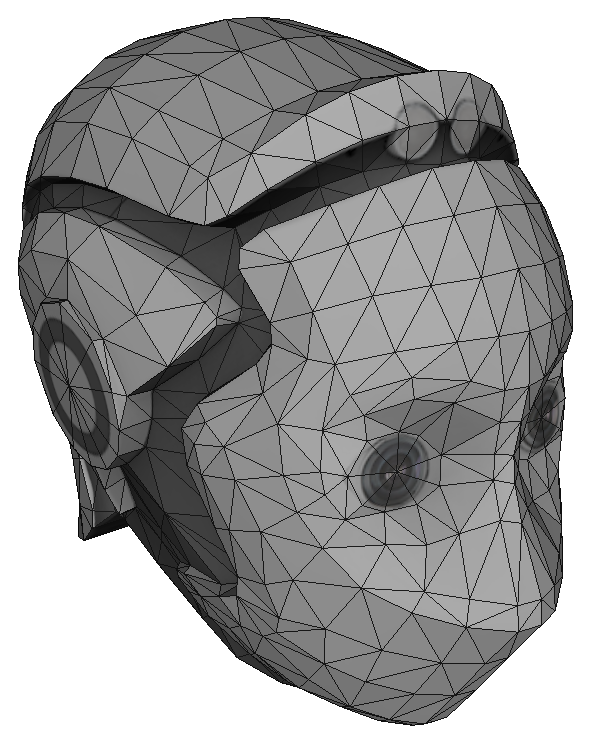
\includegraphics[width=0.3\textwidth]{../figures/mesh_head.png}
    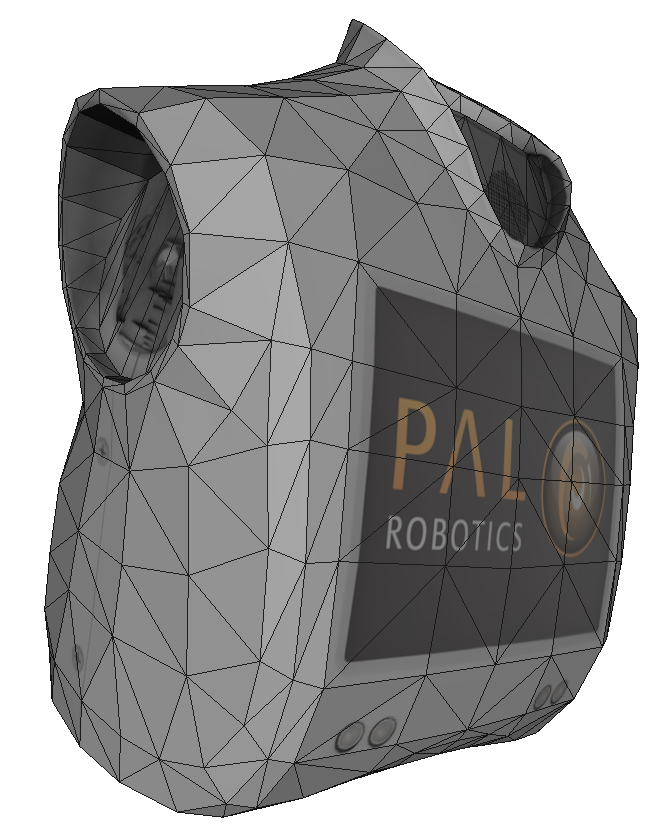
\includegraphics[width=0.3\textwidth]{../figures/mesh_torso.png}
    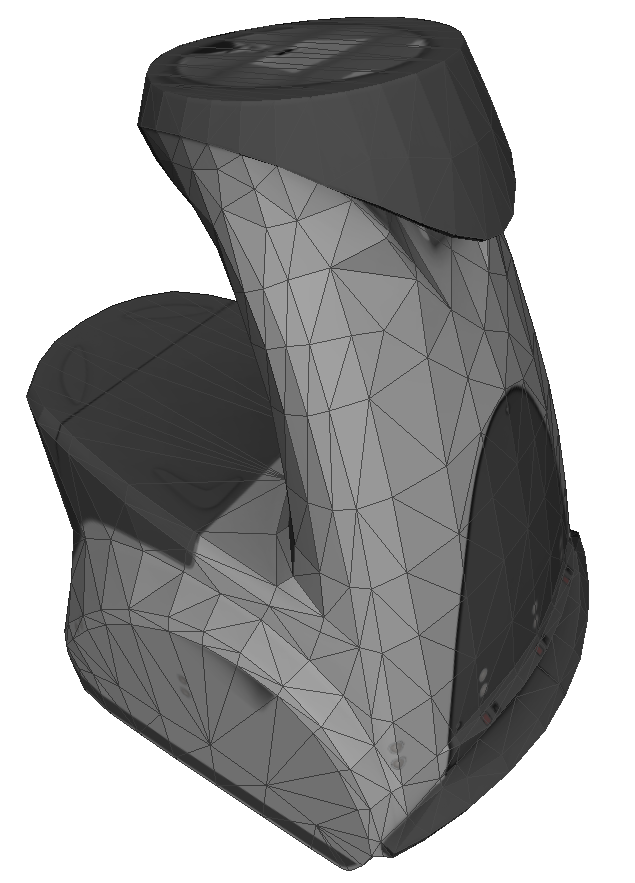
\includegraphics[width=0.3\textwidth]{../figures/mesh_base.png}
    \caption{Example for high resolution meshes. It can be easily seen, that a high number of the same normal vectors exist on the meshes. This makes a parallel configuration quite likely and the closest points can jump discontinuously.}
    \label{figmeshambiguity}
\end{figure}

\subsection{Collision Geometry - Capsule}\label{subsec:capsulecalculation}
To overcome the discontinuities mentioned in the previous section, we implemented a complete capsule decomposition for this work. A capsule describes a 3-dimensional geometry object, which consists of a cylinder along a 3-dimensional main axis and a length $l$ and radius $r$. In difference to the cylinder, each capsule comprises a half sphere at both ends of the cylinder. Since capsules are pseudo convex collision geometries, the probability of discontinuities is relatively low. There exists exactly one configuration, where ambiguity can occur. Essentially this happens, when the main axis of both capsules are parallel. Figure \ref{capsulecapsule} expresses two possible configuration for closest point pairs. It can be seen that as long as the main axis are not parallel aligned, both capsules can be treated as strictly convex objects. This convexity results in a unique point pair. \\
Furthermore, a capsule decomposition allows a smoother continuous trajectory compared to mesh to mesh calculation. In the case of parallel main axis, the dimension of possible discontinuities compared to meshes is limited to one dimension along the main-axis 
\begin{equation}
	\vec{p_i} + l_i  \vec{n} \quad i \in [CP_1,CP_2], l \in \mathbb{R}, \vec{n} \in \mathbb{R}^3
\end{equation}
where $p_i$ describes the start point of the cylinder with $z=0$, $l_i$ the length of the capsule and $n$ the orientation of the main axis. Note that in this specific case, we do not differentiate $n_{C1}$ and $n_{C2}$ as both capsules are considered to be parallel and the $z$ component is pointing along the axis. 
\newpage
Given this definition, the distance of possible discontinuities can be formulated as
\begin{eqnarray}
	\vec{p_1}	 + l_1  \vec{n} &=& \vec{p_2} + l_2  \vec{n} \\
	\vec{p_1} + l_1 \vec{n} - (\vec{p_2} + l_2 \vec{n}) &=& 0 \\
	(p_{z1} + l_1) &-& (p_{z2} + l_2) \label{eqnz}
\end{eqnarray}

where in equation \ref{eqnz}, only the $Z$ component has to be considered. $X$ and $Y$ are equal, since the two capsules are parallel.
\begin{figure}[h!]
\centering     %%% not \center
\subfigure[Unique solution]{\label{fig:capsulea}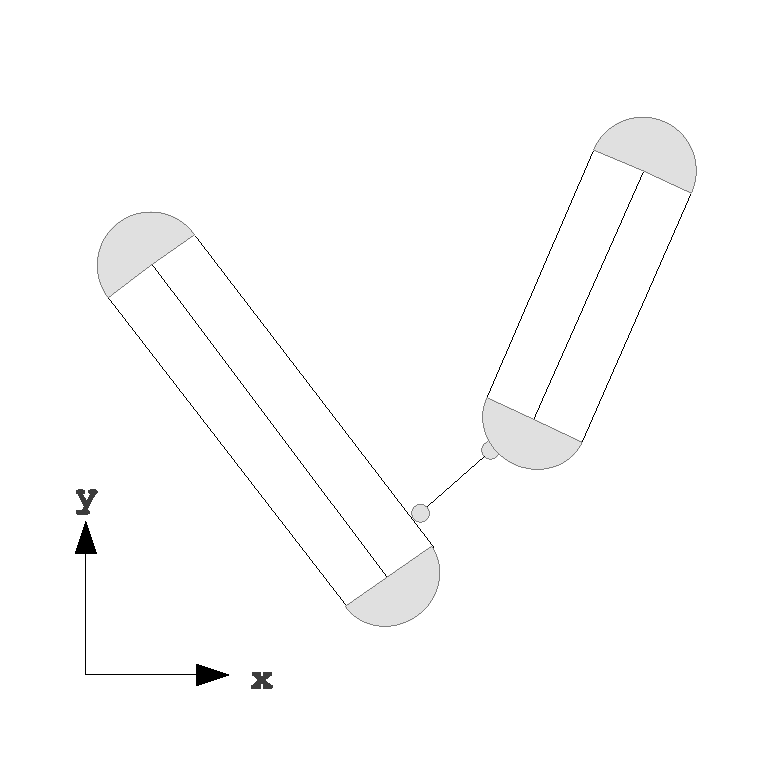
\includegraphics[width=0.48\textwidth]{../figures/capsulecapsule.eps}}
\subfigure[Parallel configuration]{\label{fig:capsuleb}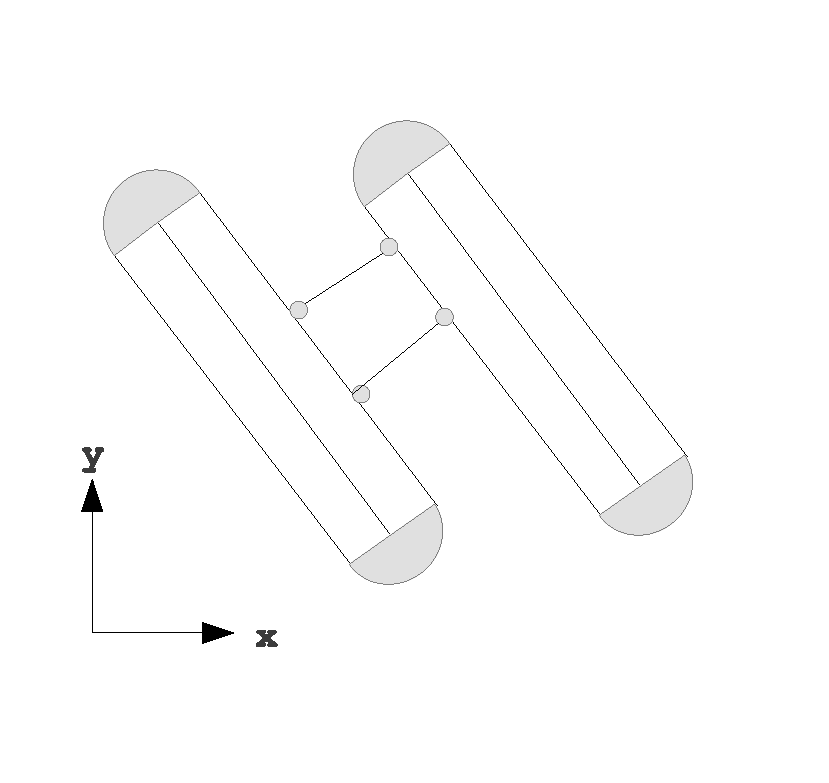
\includegraphics[width=0.48\textwidth]{../figures/capsulecapsule_parallel.eps}}
\caption{a) shows a unique solution of a closest point pair. b) shows two capsules in a parallel configuration. Note that in comparison to meshes, the ambiguity spans only along the main axis of the capsules. In a continuous motion of both capsules, these discontinuities are from no further importance, because the probability is rather low.} 
\label{capsulecapsule}
\end{figure}

\subsection{Closest Point Pair for Capsule-Capsule}
We concluded in the previous section \ref{subsec:capsulecalculation}, that a capsule decomposition of collision objects is to be preferred over meshes, because of the reduction of discontinuities. In this section, we describe the algorithm for the actual computation of the closest point pair. The presented algorithm is a derivative of the closest points based on two line segments as it is verbosely described in \cite{Ericson:2004:RCD:1121584}. Since we define a capsule to be a finite line segment in $\mathbb{R}^3$ with spatial radius information, we can modify the line segment algorithm to fit the calculated point on the surface of the capsule.

\subsubsection*{Infinite Lines}
We start our calculation by looking at the closest point calculation of two lines. According to \cite{Ericson:2004:RCD:1121584}, we formulate a line pair in $\mathbb{R}^3$ as follows.
\begin{eqnarray} \label{eqnline}
LS_1(s) &=& \vec{p_1} + s\vec{d_1} \notag\\
LS_2(t) &=& \vec{p_2} + t\vec{d_2}\notag \\
\textit{where } && \vec{d_i} = \vec{q_i} - \vec{p_i}
\end{eqnarray}
The start- and endpoint are declared as $\vec{p}$ and $\vec{q}$ in $\mathbb{R}^3$, respectively. $\vec{d}$ indicates the directional vector between $\vec{p}$ and $\vec{q}$. We find a solution for a closest point pair $s,t$, whose vector 
\begin{equation}\label{lsvec}
\vec{v}(s,t) = LS1-LS2
\end{equation}
gets minimal in length. Example is given in figure \ref{fig:lsa}.

The shortest vector $\vec{v}(s,t)$ can be examined as the scalar product of the two lines. Since the vector has to be perpendicular to both lines, the following equation system for the scalar product can be formulated:
\begin{eqnarray}
\vec{d_1} \vec{v}(s,t)&=& 0  \notag \\
\vec{d_2} \vec{v}(s,t)&=& 0  
\end{eqnarray}
we solve this equation system by substituting $\vec{v}(s,t)$ with the definition of \ref{lsvec}. Further steps are invoked:
\begin{eqnarray}
\vec{d_1} (LS_1-LS_2) &=& \vec{d_1} ((\vec{p_1}-\vec{p_2}+s\vec{d_1}- t\vec{d_2}) = 0  \notag \\
\vec{d_2} (LS_1-LS_2) &=& \vec{d_2} ((\vec{p_1}-\vec{p_2}+s\vec{d_1}- t\vec{d_2}) = 0
\end{eqnarray}
\begin{eqnarray}
(\vec{d_1}\vec{d_1})s - (\vec{d_1}\vec{d_2})t &=& -\vec{d_1}k \notag \\
(\vec{d_1}\vec{d_2})s - (\vec{d_2}\vec{d_2})t &=& -\vec{d_2}k
\end{eqnarray}
where $k= \vec{p_1}-\vec{p_2}$.
Using Cramer's rule \cite{cramer1750introduction} for solving 2x2 linear equation system finally yields the solution for $s$ and $t$:
\begin{eqnarray}
s&=& (b f - c e) / d \notag \\
t &=& (a f - b e) / d 
\end{eqnarray}
where $a = \vec{d_1^2}, b = \vec{d_1 d_2}, c = \vec{d_2^2}, e = \vec{d_1}k, f = \vec{d_2}k, d=  \vec{d_1^2}\vec{d_2^2}- (\vec{d_1 d_2})^2$ \\
Special care has to be taken in case $d=0$, which means that both lines are parallel.

\subsubsection*{Line Segments}
Compared to lines, line segments are of finite length. This necessitates a case differentiation of the spatial pose relation between two line segments. For this, we simply restrict the length along the directional vector in the range from 0 to 1.
Thus, we modify equation \ref{eqnline} according to:
\begin{equation}
LS_i(s) = \vec{p_i} + s\vec{d_i} \quad \textit{where } \vec{d_i} = \vec{q_i} - \vec{p_i}, 0 \leq s \leq 1
\end{equation}

With this formulation, we cannot apply the solution used in the previous section, as there might not be a perpendicular vector $v$ for all configurations. This situation happens, when at least one line segments lies outside the line segment of the other. In the following, we examine four different cases as illustrated in figure \ref{figlinesegments}.

When a configuration occurs as shown in figure \ref{fig:lsa}, we can apply the solutions as if the two line segments were infinite lines. When one closest point $CP_1$ lies outside its line segments, yet inside the segment of the corresponding other line, we can clamp $CP_1$ to the end of the line segment and compute the minimum distance to $LS_2$, in order to find $CP_2$. This behavior is illustrated in figure \ref{fig:lsb}. In case both closest points lie outside the corresponding line segments (see figure \ref{fig:lsc}, the procedure of \ref{fig:lsb} has to be repeated twice. We first clamp $CP_1$ to the end point and calculate $\hat{CP_2}$ . As depicted in figure \ref{fig:lsc}, this point lies outside $LS_2$ and results in a invalid point. To overcome this issue, we clamp $\hat{CP_2}$ to the endpoint of $LS_2$ and repeat the computation now inverse. We recompute $CP_1$ and see that this lies now inside $LS_1$. Figure \ref{fig:lsd} illustrates the very extreme, where both points are clamped to their respective end points.

\begin{figure}[h!]
\centering     %%% not \center
\subfigure[]{\label{fig:lsa}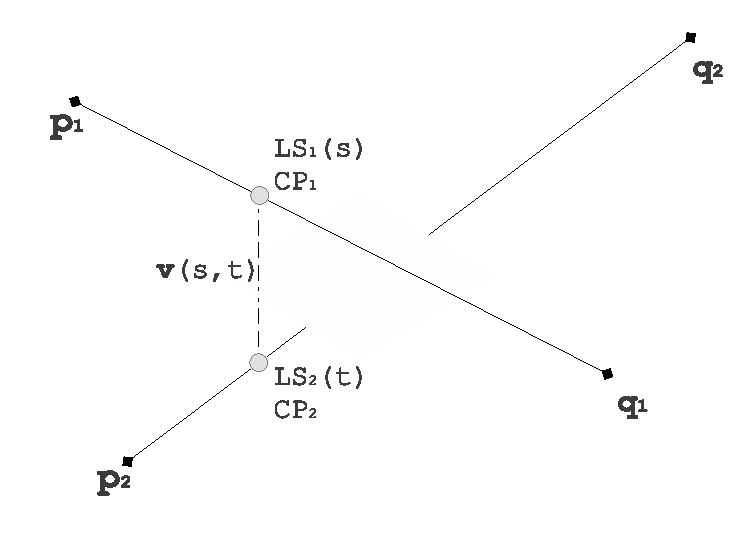
\includegraphics[width=0.4\textwidth]{../figures/linesegments1.eps}}
\subfigure[]{\label{fig:lsb}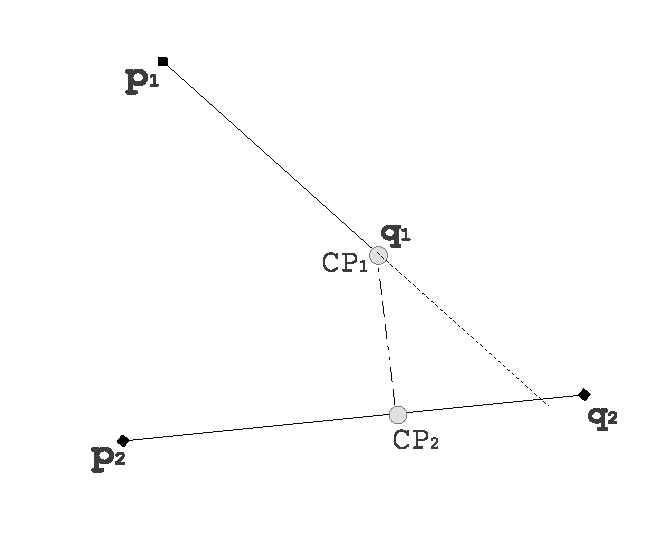
\includegraphics[width=0.4\textwidth]{../figures/linesegments2.eps}}
\subfigure[]{\label{fig:lsc}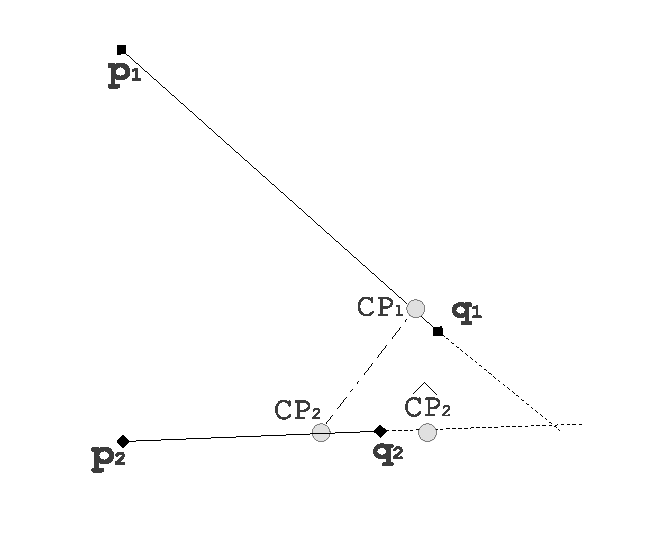
\includegraphics[width=0.4\textwidth]{../figures/linesegments3.eps}}
\subfigure[]{\label{fig:lsd}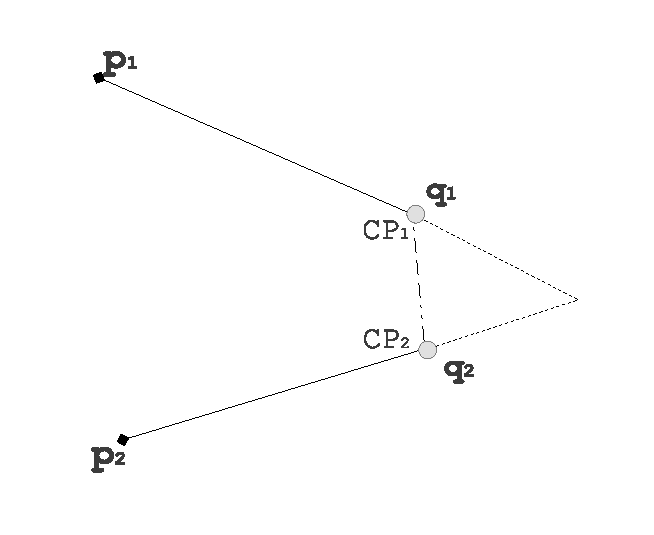
\includegraphics[width=0.4\textwidth]{../figures/linesegments4.eps}}
\caption{Relative spatial poses between two line segments. a) closest point pair lies inside both segments. b) endpoint $q_1$ is a closest point, the second closest point lies on the line segment. c) both closest points would lie outside their corresponding line segments. Here, a recursive clamping has to be implemented. d) both ending points $p_1$ and $p_2$ are closest points. } 
\label{figlinesegments}
\end{figure}

Finally, the solving process is separated in two parts. Firstly, we have to decide for the clamping of the respective points. This case study is examined according to the above description. Secondly, once the points are clamped, we can mathematically solve for the closest points.\\
We have a point $LS_2$ lying on the second segment:
\begin{equation}
LS_2(t) = \vec{P_2} + t\vec{d_2}
\end{equation}
The first point $LS_1$ is found via:
\begin{eqnarray}
LS_1(s) &=& \vec{P_1} + s\vec{d_1} \notag \\
s &=& (LS_2(t) -  \vec{P_1})\vec{d_1} / \vec{d_1}\vec{d_1} \notag \\
  &=& (\vec{P_2}+ t\vec{d_2}-\vec{p_1}\vec{d_1}/ \vec{d_1}\vec{d_1}
\end{eqnarray}
Obviously, this formulation also determines $LS_2$, given $LS_1$.

\subsubsection*{Capsules}
In the beginning of this chapter, we defined a capsule as a line segment with a spatial radius. For the closest point computation on two capsules, we enhance the algorithm for line segments slightly to project the closest on the border of the capsule.\\
As we know the two closest points $\hat{\vec{CP_1}}$ and $\hat{\vec{CP_2}}$ of the two respective line segments, we can use this information to calculate the directional vector between them. The projection is to the border of the capsule is done by shifting the closest points along this vector by the radius. Figure \ref{fig:capsulevec} shows this projection.
\begin{figure}[h!]
  \centering
    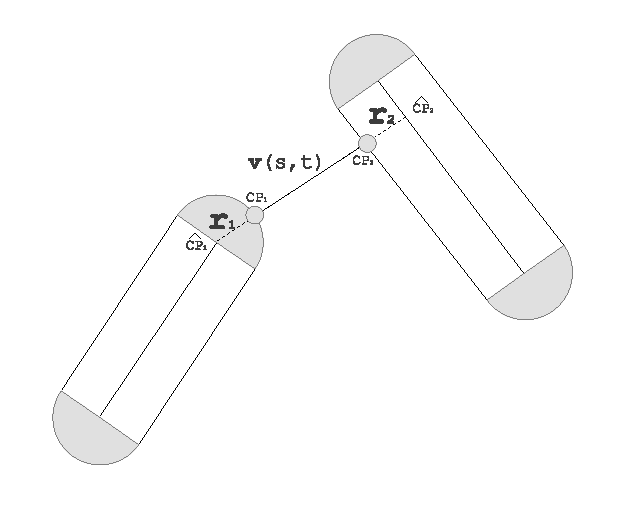
\includegraphics[width=0.7\textwidth]{../figures/capsulecapsule_vector.eps}
    \caption{Projection of the two closest points $\hat{\vec{CP_1}}$ and $\hat{\vec{CP_2}}$ to the border of the capsule. $\vec{v(s,t)}$ describes the directional vector along which the projection is done with length $r_i$.}
    \label{fig:capsulevec}
\end{figure}

We can formulate this solution, given the two closest points $\hat{\vec{CP_1}}, \hat{\vec{CP_2}}$. We calculate the vector $\vec{v}$:
\begin{equation}
\vec{v} = \hat{\vec{CP_2}}-\hat{\vec{CP_1}}
\end{equation}
The shifting is done via:
\begin{eqnarray}
\vec{CP_1} &=& \hat{\vec{CP_2}} + r_1 \vec{v} \notag \\
\vec{CP_1} &=& \hat{\vec{CP_1}} - r_2 \vec{v} \notag \\
\end{eqnarray}

\section{Velocity Damping}\label{sec:velocitydamping}
In section \ref{chapter:soth} we pointed out that every task has to be designed in the form of 
\begin{equation}
\vec{Ax-b} \quad  \vec{A} \in \mathbb{R}^{m \times n}, \vec{x} , \vec{b} \in \mathbb{R}^{m}
\end{equation}
In this section, we introduce the task formulation for collision avoidance. The collision avoidance task restricts any possible movement along the unitvector between the closest point pair, we calculated in the previous section. The presented approach was firstly introduced in \cite{Faverjon87alocal} and reformulated inside the SoT \cite{Kanehiro-RSS08}. 
As we have seen in equation \ref{eqn:ikleastsquare}, controlling a body part in cartesian space corresponds to the IK formulation  
\begin{equation}\label{gototask}
\vec{J(p,q) \dot{q} - \dot{x}} \quad  \vec{J} \in \mathbb{R}^{m \times n}, \vec{\dot{q}, \dot{x}} \in \mathbb{R}^{n}
\end{equation}
where $\vec{J(p,q)}$ names the Jacobian of point $\vec{p}$ at joint vector position $\vec{q}$, the resulting joint velocities $\vec{\dot{x}}$ and the cartesian goal velocity. This formulation solves for all available DoF inside the hierarchy. In order to restrict the solution for one direction, we modify the above formulation in two aspects.
\begin{itemize}
	\item The Jacobian is projected onto the unitvector spanned by the closest point pair
	\item The task is formulated as an inequality, which introduces a lower boundary for the proximity (distance) of the two body parts
\end{itemize}

\subsection{Jacobian Projection}
The configuration setup according to \cite{Faverjon87alocal} is depicted in figure \ref{figcapsuledistance}. The figure shows a close up view of a capsule pair, with closest points $\vec{p_1}$ and $\vec{p_2}$. Hereby, we consider the point $\vec{p_1}$ as the moving body part, whereas $\vec{p_2}$ is meant to be fixed\footnote{We establish the task with this convention of $\vec{p_2}$ being fixed in space. However, the implementation necessarily allows both points to be moving.} in $\mathbb{R}^3$ as a collision object. The unitvector $\vec{n}$ is defined as
\begin{equation}
	\vec{n} = \vec{\frac{p_1-p_2}{\Vert p_1 - p_2 \Vert}}
\end{equation}

The distance is computed according to the euclidean L2-Norm:
\begin{equation}
	d = \Vert \vec{p_1-p_2} \Vert = \sqrt[2]{(\vec{p_1-p_2})^2}
\end{equation}

\begin{figure}[h!]
  \centering
    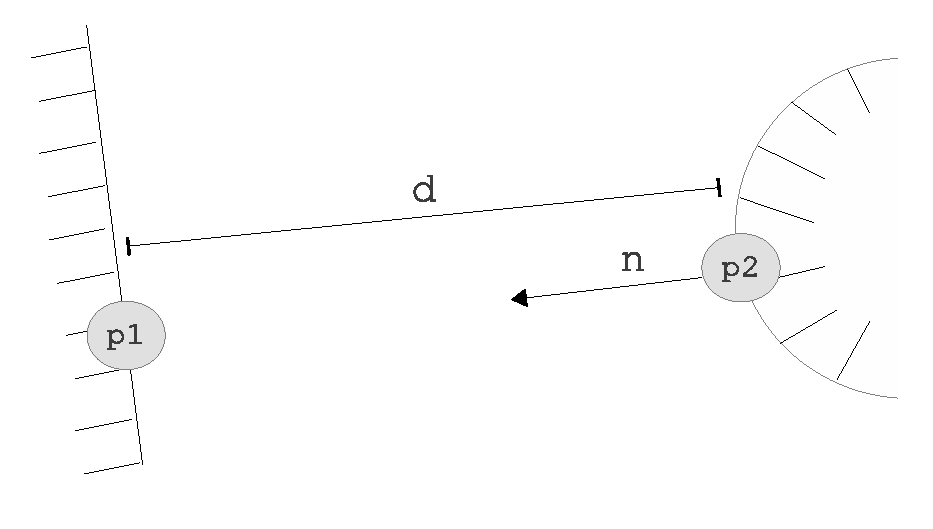
\includegraphics[width=0.8\textwidth]{../figures/capsuledistance.eps}
    \caption{A close up view of two capsules. The unitvector $n$ is pointing from $p_2$ to $p_1$. The distance $d$ corresponds to the euclidean L2-norm of $p_1$ and $p_2$.}
    \label{figcapsuledistance}
\end{figure}

To begin with, we modify the task definition in equation \ref{gototask} to restrict only the projection along $n$. Thus, the new task formulation becomes
\begin{equation}\label{gototaskn}
\vec{n^TJ(p_1,q) \dot{q} - \dot{x}} \quad ,\vec{n} \in \mathbb{R}^m, \vec{J} \in \mathbb{R}^{m \times n}, \vec{\dot{q}} , \vec{\dot{x}} \in \mathbb{R}^{m}
\end{equation}
where $\vec{n^T}$ describes the scalar product of $\vec{n}$ and $\vec{J}$. Informally spoken, we can treat the scalar product as the projection of the Jacobian onto the unitvector pointing towards the collision center. Note that we annotate the Jacobian parameters with respect to $p_1$. With this, we indicate, that the Jacobian has to be calculated in respect to the closest point $p_1$. The next section \ref{sec:jacobian} gives a more detailed examination on it.

\newpage
\subsection{Inequality Formulation}
To avoid a possible collision between two capsules, we have to ensure that the distance between them will always be larger than zero. To guarantee a minimal distance threshold, we transform the task in equation \ref{gototaskn} into an inequality constraint. Furthermore, we introduce a lower bound with respect to the actual distance. The outer circle in figure \ref{figcapsuledistanceds} represents this lower bound, where the minimal proximity of the point pair $\vec{p_1}$,$\vec{p_2}$ has to be larger than $d_s$.
\begin{figure}[h!]
  \centering
    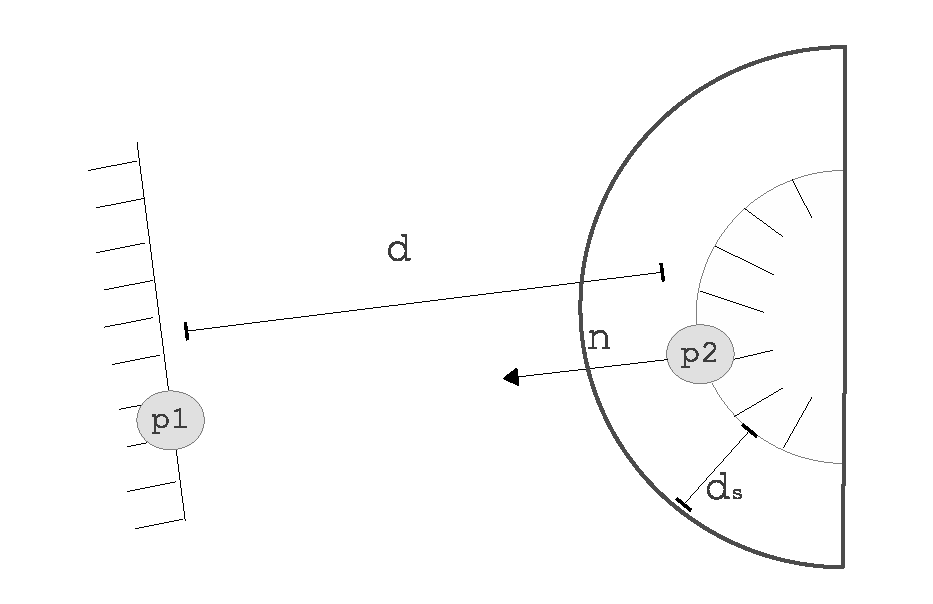
\includegraphics[width=0.8\textwidth]{../figures/capsuledistanceds.eps}
    \caption{To ensure a minimal proximity between two capsules, a security distance $d_s$ is introduced. The closest point $\vec{p_1}$ has to be outside the distance zone.}
    \label{figcapsuledistanceds}
\end{figure}
The solution space for this inequality task is formulated in respect to the current distance $d$. Thus, the equation \ref{gototaskn} evolves to an inequality constraint
\begin{equation}\label{gototaskds}
\vec{n}^T\vec{J(p_1,q)} \vec{\dot{q}} \geq - \epsilon \frac{d - ds}{\Delta t}\quad , \epsilon, d, d_s, \Delta t \in \mathbb{R}
\end{equation}
where $d-d_s$ calculates the distance along $\vec{n}$. The velocity towards the collision center undergoes a damped course, hence the name velocity damping.
We stress out the $\Delta t$ in equation \ref{gototaskds} to demonstrate the calculation in the velocity domain. In the implementation although, this value is not available as a parameter, since the control gain value $\epsilon$ has to be tuned for each application, which may compensate for $\Delta t$. \\
We can see that the velocity converges to zero with decreasing proximity between the closest point pair.
\begin{equation}
\lim\limits_{d \rightarrow d_s}{- \epsilon\frac{d - ds}{\Delta t} = 0}
\end{equation}
\newpage
We can now formulate the overall optimization problem as a task space formulation where a position $\vec{x_d}$ is specified as a goal position and $\vec{x}$ the current cartesian position. The optimization of this task is now subject to the velocity damping constraint developed in this section. The verbose formulation of the QP looks as the following:
\begin{eqnarray}
\underset{\vec{\dot{q}}}{\text{min}} \rightarrow \Vert \vec{J(p_x,q) \dot{q} - \dot{x}} \Vert^2  \notag \\
\underset{\vec{\dot{q}}}{\text{min}} \rightarrow \Vert \vec{J(p_x,q) \dot{q}} - \frac{(\vec{x-x_d})}{\Delta t} \Vert^2  \\
\text{subject to} \quad \vec{n}^T\vec{J(p_1,q)} \vec{\dot{q}} \geq - \epsilon \frac{d - ds}{\Delta t} \label{eqn:taskdampconstraint}
\end{eqnarray}

One note to the above formulation: It might look counter-intuitive at a first glance to design the task like this. One would presume a twist in the directions of $\vec{n}$ as well as the preceding minus sign in equation \ref{gototaskds}. It is more intuitive to assume $\vec{n}$ to point from $\vec{p_1}$ to $\vec{p_2}$. This modulation comes directly from the architecture of the hierarchical solver as a first-order control system. We review again the derivation of a task in cartesian space, which is depicted in the diagram \ref{fig:ikcontrolloop}.
\begin{eqnarray}
\vec{J(q)\dot{q}} &=& \vec{\dot{x}} \notag \\
\vec{J(q)\dot{q}} &=& K \frac{\vec{x - x_d}}{\Delta t} \label{eqnplus}  \\
\vec{J(q)\dot{q}} &=& -K \frac{\vec{x_d - x}}{\Delta t} \label{eqnminus}  \\
\vec{\dot{x}} &\equiv& - \hat{K} \vec{x_e} \quad, \text{where } \hat{K}= \frac{k}{\Delta t} \label{eqnfirstorder}
\end{eqnarray}
We can see from the above formulation that between equation \ref{eqnplus} and equation \ref{eqnminus} the sign changed as the formulation of the error between $\vec{x}$ and $\vec{x_d}$ swapped. Finally, \ref{eqnfirstorder} results in a common first-order control system formulation. The velocity damping task obeys this formulation.

\subsection{Integration into Hierarchy Solver}
The QP formulation represents an example for one collision pair. Equation \ref{eqn:taskdampconstraint} describes an inequality constraint for one closest point pair $\vec{p_1}$,$\vec{p_2}$ and the according distance $d$.\\
Obviously regarding the self-collision avoidance, we have to extend this to integrate multiple velocity damping constraints.
Depending on the application, it might be important on which level these inequality constraints are placed inside the solver hierarchy. This further depends which relative level the damping constraints have to each other inside the hierarchy. We can consider two cases:

\begin{itemize}
\item Constraints are on the same level
\item Constraints are on different level
\end{itemize}

\subsubsection*{Same Level}
Looking at self-collision avoidance, it is necessary that all collision pairs are on an equal level inside the solver hierarchy. This comes with no surprise, as one would expect the left arm being equally treated as the right arm in terms of avoiding self-collision. \\
To achieve this, we can concatenate the formulation given in \ref{eqn:taskdampconstraint}. For multiple collision points inside one task, the formulation evolves to:
\begin{equation}
\vec{n_i}^T\vec{J(p_{1,i},q)} \vec{\dot{q}} \geq - \epsilon_i \frac{d_i - d_{s,i}}{\Delta t} \quad \forall i \in \textit{\{1, \dots ,k\} }
\end{equation}
where $i$ iterates over all $k$ available collision pairs, which are considered to be on the same level. Written in matrix notation, this yields to

\begin{eqnarray}
\begin{pmatrix}
 \vec{n_1}^T\vec{J_1} \\
 \vdots \\[0.5em]
 \vec{n_k}^T\vec{J_k}
\end{pmatrix} 
 \vec{\dot{q}} &\geq &
 \begin{pmatrix}
 \vec{\dot{d_1}} \\
 \vdots \\[0.5em]
 \vec{\dot{d_k}}
\end{pmatrix} \notag \\
\vec{N} \vec{\dot{q}} &\geq & \vec{D} \notag \\
\textit{where } \vec{J_i} &=& \vec{J(p_{1,i},q)} \notag \\
\textit{and } \vec{\dot{d_i}} &=& \frac{d_i - d_{s,i}}{\Delta t}
\end{eqnarray}
Again the complete QP respecting all constraints at the same level yields:
\begin{eqnarray}
\underset{\vec{\dot{q}}}{\text{min}} \rightarrow \Vert \vec{J(p_x,q) \dot{q} - \dot{x}} \Vert^2  \notag \\
\text{subject to} \quad \vec{N}\vec{\dot{q}} \geq \vec{D} \label{eqn:taskdampconstraintsamelevel}
\end{eqnarray}


\subsubsection*{Different Level}
There may be applications, where multiple hierarchy steps are feasible. One could think of setting priority to self-collision avoidance over external collision avoidance. In this case, no further modifications have to be implemented for the task itself. This approach can simply be realized by stacking the two instances of the velocity damping task on top of each other.

\section{Jacobian Calculation for Closest Point}
 \label{sec:jacobian}
The task formulation examined in the previous section \ref{sec:velocitydamping} constrains one closest point pair. Hence, we can see in equation \ref{gototaskds} the subscript for $\vec{p}$ as a parameter for the Jacobian $\vec{J}$. We concluded in section \ref{sec:closestpoints} that based on the pseudo convexity of capsules as collision geometries, the closest point pairs move along a differentiable trajectory. On the same hand, this means that for each iteration of the solver, a new Jacobian has to be computed since we parameterize the Jacobian with $\vec{p},\vec{q}$
\begin{equation}
\vec{J} \equiv \vec{J}(\vec{p,q}) \equiv \vec{J}(\vec{p}(t),\vec{q}(t))
\end{equation}

\subsection{Jacobian Calculation for Rigid Body Parts}
To begin with, we introduce a short review for the general case of computing the Jacobian matrix for rigid body parts. The experienced reader might freely skip this section. During this section, we mainly stick to the notation convention
as suggested in \cite{citeulike:1090825}. \\

Forward kinematics (FK) describes the function $f$ of translating a n-dimensional joint position vector $q$ into 6-dimensional cartesian poses. Similarly, \textit{Differential} kinematics maps joint velocities to cartesian velocities, namely linear velocity $\vec{\dot{p}}$ and angular velocity $\vec{\omega}$. Hereby, there exists a linear relation between joint velocities and cartesian velocities:
\begin{eqnarray}
\vec{P} &=& f(\vec{q}) \vec{q} \notag \\[1em]
\vec{\dot{P}} &=& \frac{\delta f(\vec{q})}{\delta \vec{q}} \vec{\dot{q}} \notag \\
\vec{\dot{P}} = 
\begin{bmatrix}
\vec{\dot{p}} \\
\vec{\omega} 
\end{bmatrix} &=& \vec{J} \vec{\dot{q}} \notag \\
\textit{ where } && \vec{P} \in \mathbb{R}^{6 \times n} , \vec{J} \in \mathbb{R}^{6 \times n}, \vec{\dot{q}} \in \mathbb{R}^n\label{eqn:jacobianmap}
\end{eqnarray}

From the FK, we know the following relation:
\begin{equation}
\vec{p_i} = \vec{p_{i-1}} + \vec{R}_{i-1}\vec{r_{i-1,i}^{i-1}} \label{eqn:linkposition}
\end{equation}
where $\vec{p_i,p_{i-1}}$ denote the current position vector of frame origin $i$ and $i-1$, respectively. $\vec{R}_{i-1}$ describes the rotation matrix of frame $i-1$, whereas $\vec{r_{i-1,i}^{i-1}}$ denotes the relative translation from frame origin $i-1$ to $i$. The relation is illustrated in \ref{fig:linkvelocity}

\begin{figure}[h!]
  \centering
    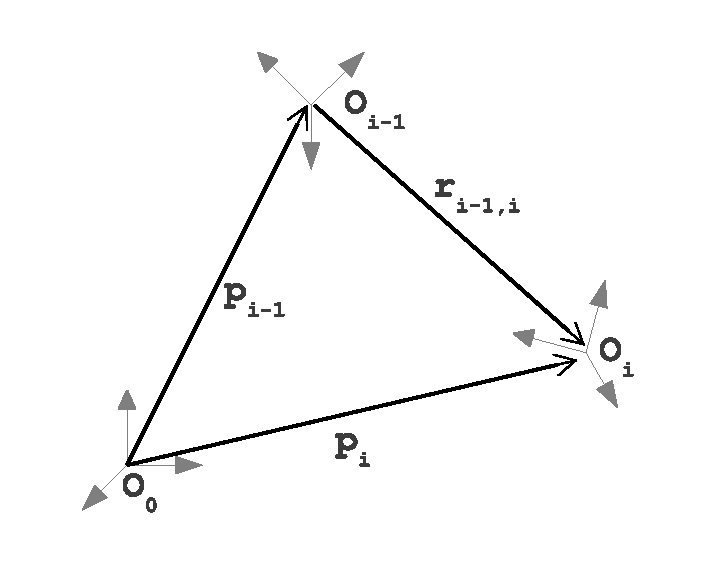
\includegraphics[width=0.6\textwidth]{../figures/link_velocity.eps}
    \caption{Relative position between two origin frames expressed in a common base frame.}
    \label{fig:linkvelocity}
\end{figure}

\subsubsection*{Linear Velocity}
For obtaining the according linear velocity formulation, we can take the first derivative of the above equation \ref{eqn:linkposition}. This yields into:
\begin{eqnarray}
\vec{\dot{p_i}} &=& \vec{\dot{p}_{i-1}} + \vec{R}_{i-1}\vec{\dot{r}_{i-1,i}^{i-1}} + \vec{\omega}_{i-1} \times \vec{R}_{i-1}\vec{r_{i-1,i}^{i-1}} \notag \\
&=& \vec{\dot{p}}_{i-1} 
+ \vec{v}_{i-1,i} + 
\vec{\omega}_{i-1} \times \vec{r}_{i-1,i}
\end{eqnarray}
Hereby, the linear velocity is split into translational velocity $\vec{v}$ and rotational linear velocity $\vec{\omega}_{i-1} \times \vec{r}_{i-1,i}$ between two adjacent links.
\subsubsection*{Angular Velocity}
The angular velocity can be obtained from the rotation matrix composition
\begin{equation}
\vec{R_i} = \vec{R}_{i-1}\vec{R}_{i}^{i-1} \label{eqn:rotationcomp}
\end{equation}
It can be shown in \cite{citeulike:1090825} and \cite{opac-b1129198}, by useful exploiting the skew matrix property, taking the first derivative of equation \ref{eqn:rotationcomp} yields to the angular velocity formulation:
\begin{eqnarray}
\vec{\omega}_i &=& \vec{\omega}_{i-1} + \vec{R}_{i-1} \vec{\omega}_{i-1,i}^{i-1} \notag \\
&=& \vec{\omega}_{i-1} + \vec{\omega}_{i-1,i}
\end{eqnarray}

Furthermore, the relations examined in equation \ref{eqn:linkposition} and \ref{eqn:rotationcomp} differ depending on the type of joint. We have to differentiate the velocity decompositions depending whether we are considering a revolute or prismatic joint:

\subsubsection*{Revolute Joint}
According to the Denavit-Hartenberg Convention (DHC), the axis of rotation is $z$ \cite{hartenberg-1964a}. Hence, the angular velocity simplifies to
\begin{equation}
\vec{\omega}_{i-1,i} = \dot{\theta}_i \vec{z}_{i-1}
\end{equation}
where $\vec{\dot{\theta}}$ denotes the rotational joint speed. Using this, we calculate further the linear velocity:
\begin{equation}
\vec{v}_{i-1,i} = \vec{\omega}_{i-1,i} \times \vec{r}_{i-1,i}
\end{equation}
Once we computed $\vec{\omega}_{i-1,i}$ and $\vec{v}_{i-1,i}$, we finally obtain:
\begin{eqnarray}
\vec{\omega} &=& \vec{\omega}_{i-1} + \dot{\theta}_i \vec{z}_{i-1} \\
\vec{\dot{p}}_i &=& \vec{\dot{p}}_{i-1} + \vec{\omega}_i \times\vec{r}_{i-1,i} 
\end{eqnarray}

\subsubsection*{Prismatic Joint}
Equally to the revolute joints, we have to reconsider the equations of velocity for prismatic joints. Since the prismatic joint has no rotational part, the angular velocity equals zero
\begin{equation}
\vec{\omega}_{i-1,i} = \vec{0}
\end{equation}
Also for prismatic joint, the axis of movement according to DHC is along $z$. The linear velocity results to
\begin{equation}
\vec{v}_{i-1,i} = \dot{d}_i \vec{z}_{i-1}
\end{equation}
The final velocities are computed respectively:
\begin{eqnarray}
\vec{\omega} &=& \vec{\omega}_{i-1} \\
\vec{\dot{p}}_i &=& \vec{\dot{p}}_{i-1} +\dot{d}_i \vec{z}_{i-1} + \vec{\omega}_i \times\vec{r}_{i-1,i} 
\end{eqnarray}

\subsubsection*{Jacobian Calculation}
In equation \ref{eqn:jacobianmap}, we introduced the Jacobian as a mapping between cartesian space and joint space. As we have seen in the former examination, the Jacobian maps rotational and translational velocity towards cartesian velocity. Thus, we can formulate the Jacobian as such:
\begin{equation}
\vec{J} = \begin{pmatrix}
\vec{J}_p \\
\vec{J}_r
\end{pmatrix} = \begin{pmatrix}
\vec{J}_{p_{1}} & \dots & \vec{J}_{p_{n}} \\
\vec{J}_{r_{1}} & \dots & \vec{J}_{r_{n}} \\
\end{pmatrix} \quad ,\textit{with }\vec{J} \in \mathbb{R}^{6 \times n} \label{eqn:jacobiandecomposition}
\end{equation}
where each $\vec{J}_{p_{i}}$,$\vec{J}_{r_{i}}$ describes a 3-dimensional vector, which relates each joint velocity $\dot{q}_i$ to the linear velocity. $\vec{J}_{p_{i}}$ maps $x,y,z$ components of translational velocity into cartesian space. Equally $\vec{J}_{r_{i}}$ relates the orientation in terms of Euler angles $R,P,Y$. 
\begin{equation}
\vec{J}_{p_{i}} = \begin{bmatrix}
J_{p_{i,x}} \\ 
J_{p_{i,y}} \\
J_{p_{i,z}} \\
\end{bmatrix} \quad \quad
\vec{J}_{r_{i}} = \begin{bmatrix}
J_{r_{i,r}} \\ 
J_{r_{i,p}} \\
J_{r_{i,y}} \\
\end{bmatrix}
\end{equation}

In particular the mapping function looks like the following:
\begin{equation}
\begin{bmatrix}
\dot{p}_x \\
\dot{p}_x \\
\dot{p}_x
\end{bmatrix} =
\vec{J}_{p} 
\vec{\dot{q}}  \quad \quad
\begin{bmatrix}
\dot{p}_r \\
\dot{p}_p \\
\dot{p}_y
\end{bmatrix} =
\vec{J}_{r} 
\vec{\dot{q}}
\end{equation}

We can now compute the full Jacobian, taking again the different types of joints into account. We compute each pair of $\vec{J}_{p_{1}}$,$\vec{J}_{r_{1}}$ in equation \ref{eqn:jacobiandecomposition} according to:
\begin{equation}
\vec{J} = 
\begin{pmatrix}
\vec{J}_{p_{1}} \\
\vec{J}_{r_{1}}
\end{pmatrix}=\left\{
\begin{array}{l l}
\begin{pmatrix}
\vec{z}_{i-1} \times (\vec{p}-\vec{p}_{i-1}) \\
\vec{z}_{i-1}
\end{pmatrix} & \textit{for revolute joints} \\[1.7em]
\begin{pmatrix}
\vec{z}_{i-1} \\
\vec{0}
\end{pmatrix} & \textit{for prismatic joints}
\end{array} \right.
\end{equation}
For a detailed and well explained derivation of the above computation, the interested reader is referred to \cite{citeulike:1090825} and \cite{opac-b1129198}. 

\subsection{Jacobian Calculation of Moving Points}
In the previous section, calculated the Jacobian with respect to all related joints along one kinematic chain ending with the tool joint at the tip. Within this calculation, the assumption is taken that all joint position are at the end point of the link. The axis of movement is $Z$. \\
For the purpose of collision avoidance based on a closest point pair, we need the Jacobian in respect of the closest point $p_1$, which varies from the center point on the $z$-axis. As depicted in figure \ref{fig:capsulejacobian}, we need to find a transformation from the Jacobian calculated for frame origin $O_i$ to frame origin $O_{cp}$. This means, we need a mapping from the joint velocities to the linear and angular velocities at point $O_{cp}$. 
\begin{figure}[h!]
  \centering
    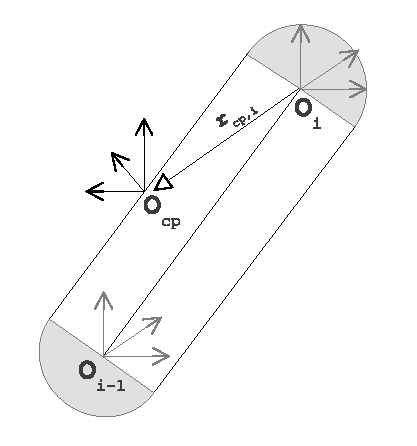
\includegraphics[width=0.3\textwidth]{../figures/capsulejacobian.eps}
    \caption{Jacobian has to be calculated in respect to frame $O_{cp}$. The coordinate frame transformation can be realized with a twist, given the relative transformation $r_{cp,i}$ between $O_i$ and $O_{cp}$. }
    \label{fig:capsulejacobian}
\end{figure}
Since the closest point is part of the capsule, for which origin we can easily calculate the Jacobian, we can treat this as a static transformation. Thus, we can state the following relation:
\begin{eqnarray}
\vec{\dot{p}_{cp}} &=& \vec{\dot{p}_i} + \vec{\omega_i} \times \vec{r}_{cp,i}  \notag \\
\vec{\omega_{cp}} &=& \vec{\omega_i}
\end{eqnarray}
By utilizing the skew-symmetric operator $S(\bullet)$, we can write the above relation in matrix notation. 
\begin{equation}
\begin{pmatrix}
\vec{\dot{p}_{cp}} \\
\vec{\omega_{cp}}
\end{pmatrix}  = 
\begin{pmatrix}
\vec{I} & -\vec{S}(\vec{r}_{cp,i}) \\
\vec{0} & \vec{I}
\end{pmatrix} 
\begin{pmatrix}
\vec{\dot{p}_{i}} \\
\vec{\omega_{i}}
\end{pmatrix} \label{eqn:twist}
\end{equation} 
This results in a twist computation as the linear projection now describes a $\mathbb{R}^{6\times6}$ matrix. We can use this formulation in order to obtain the Jacobian at point $O_{cp}$. If we substitute $\vec{\dot{p}_{cp}}$ and $\vec{\omega_{cp}}$ with the Jacobian mapping function, equation \ref{eqn:twist} yields
\begin{eqnarray}
\begin{pmatrix}
\vec{\dot{p}_{cp}} \\
\vec{\omega_{cp}}
\end{pmatrix}  &=& 
\begin{pmatrix}
\vec{I} & -\vec{S}(\vec{r}_{cp,i}) \\
\vec{0} & \vec{I}
\end{pmatrix} 
\begin{pmatrix}
\vec{\dot{p}_{i}} \\
\vec{\omega_{i}}
\end{pmatrix} \notag \\ [0.7em]
\vec{J}(\vec{p}_{cp},\vec{q})\vec{\dot{q}} &=& 
\begin{pmatrix}
\vec{I} & -\vec{S}(\vec{r}_{cp,i}) \\
\vec{0} & \vec{I}
\end{pmatrix} 
\vec{J}(\vec{p}_{i},\vec{q})\vec{\dot{q}}
\notag \\ [0.7em]
\vec{J}(\vec{p}_{cp},\vec{q}) &=& 
\begin{pmatrix}
\vec{I} & -\vec{S}(\vec{r}_{cp,i}) \\
\vec{0} & \vec{I}
\end{pmatrix} 
\vec{J}(\vec{p}_{i},\vec{q}) \label{eqn:solvejaccp}
\end{eqnarray}

With the above formulation, we can calculate the Jacobian at any point of the capsule. Most kinematic or dynamic libraries provide already the capability of computing the Jacobian along the kinematic chain up to the end effector position. Thus, for every update of the solver, we have to compute the relative transformation $\vec{r}_{cp,i}$ and obtain the according Jacobian based on equation \ref{eqn:solvejaccp}. 
		
		
		%
		%% ---------------------------------------------------------------------------
		%%
		%% Fully Automated Calibration for Ultrasound
		%%
		%%% ---------------------------------------------------------------------------
		\part[Implementation]{Implementation Details}
		\label{part:implementation}
		 
		 
		\chapter{Implementation Environment}
\label{chapter:implenv}
In this chapter, we introduce the environment used for the implementation of this work. Hereby, we provide conceptional overview about the underlying real time critical base implementation, namely ROS\_control, which serves as a generic interface between robot control and respective hardware. At this point, we assume the reader to be familiar with ROS. A good introduction, tutorials and detailed information can be found in \cite{martinez2013learning} and the official website\footnote{\url{http://www.ros.org/}}.

Furthermore, we introduce the SoT as a framework in terms of implementing tasks and dynamically push and pop them on runtime. Hereby, we describe the Dynamic Graph (DG). This serves as a computational graph and each task can be seen as one entity inside this graph.

Latest, the closest points are calculated utilizing an open-source library called Fast Collision Library (FCL), which brings already mechanisms for calculating proximities. During this work, the capabilities of this library is extended for capsules. 

\section{ROS\_control}\label{sec:roscontrol}
In a wide sense, ROS\_control describes a combination of packages for building robot agnostic controllers. It provides interfaces for controllers and various hardware systems to generically separate the controllers from the underlying hardware. ROS\_control thus can be seen as a hardware abstraction layer (HAL). On the upper side, ROS\_control enables a generic ROS compatible programming interface, which allows hardware agnostic computation of various application algorithms. On the lower side, it communicates in a real time safe environment with the concrete hardware. This mechanism is monitored by a independent observer, called the controller manager, which allows to load, switch and unload multiple controllers on runtime. More information can be found in \cite{roscontrol}.

During the development of this work, we implemented a so-called SoT-Controller and integrated it into ROS\_control. This integration implies a seamless migration and execution on the real robot hardware through the implemented HAL for REEMs hardware.
To overcome any real time constraints inside the computation of the stack, we exposed this computation into a separate thread. This not just detaches the SoT from any hard timing condition, but rather allows us to modify the update frequency inside the SoT independently from ROS\_control. At each \texttt{update} function call of the SoT-Controller, it fetches the latest result $q$, representing the accumulated joint states. Those joint state values are passed through a \texttt{joint position controller} and finally to the robots motor controllers. This abstract description is illustrated in figure \ref{fig:sotcontrol}.
\begin{figure}[h!]
  \centering
    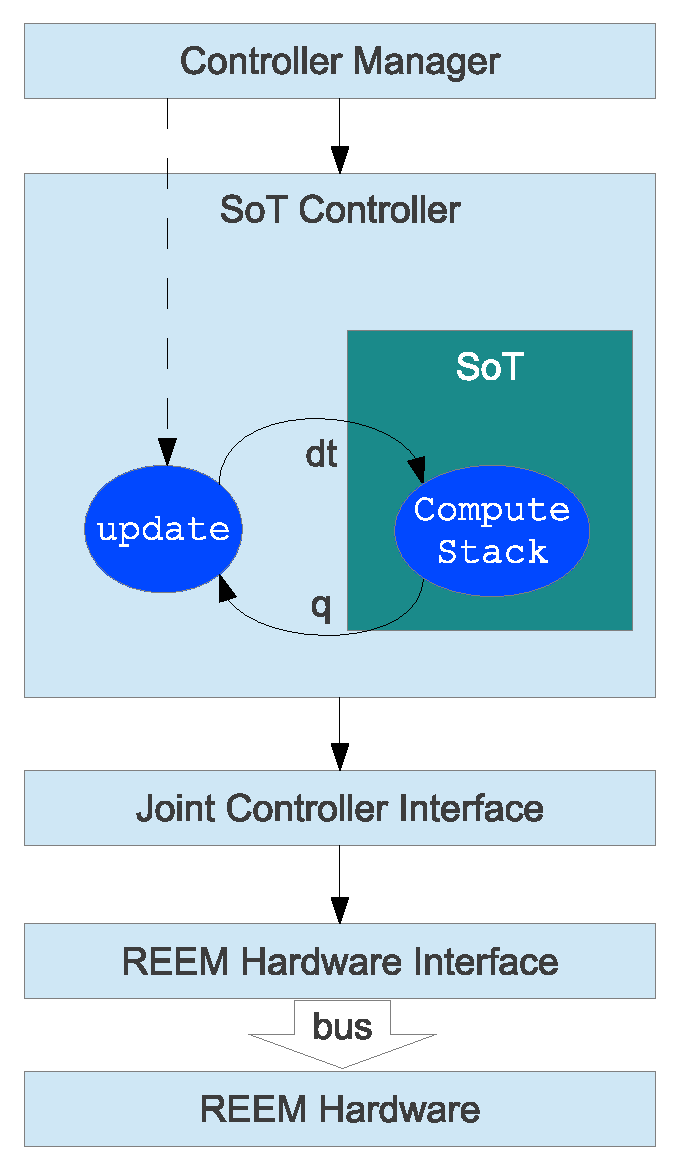
\includegraphics[width=0.4\textwidth]{../figures/sot_controller.eps}
    \caption{Abstract overview of the SoT-controller architecture inside ROS\_control. The controller manager cyclically calls the \texttt{update} function for all subscribed controllers. This update function fetches the latest result from the independently running SoT. The joint states are getting passed over various interfaces finally to the communication bus and the respective motor control boards.}
    \label{fig:sotcontrol}
\end{figure}

\section{Stack of Task - Framework}\label{sec:sotframework}
During the theoretical part in chapter \ref{chapter:soth}, we introduce the SoT as a GIK solver and provide mathematical formulations on how to define a task inside this solver. In this section, we consider the SoT from a software framework point of view. With this being said, in the remainder of this section, the use of the abbreviation SoT refers to the framework rather than the hierarchical solver. 

The SoT comprises mainly two key functionalities. 
\begin{itemize}
\item Dynamic computational graph connecting entities through input/output signals
\item Hierarchical task solver (called sot-core) realized as entities inside the dynamic graph
\end{itemize}

\subsection{Dynamic Graph}
The dynamic graph (DG) provides a computational graph, where entities are connected through input and output signals \cite{mansard:icar:09}. Hereby, every output signal is combined with an internal function of the entity, gathering all necessary information. This happens by consuming the input signals and produce the result on the output signal. Output signals from one entity can be plugged as an input signal of any other entity. 

For every cycle of the control update loop, the DG gets recomputed based on backtracking all linked entities. Triggering an output signal executes the assigned output function inside the entity. Equally, this function might consume linked input signals. Since these input signals represent output signals of other entities, those entities are computed as well. Let us consider the DG illustrated in figure \ref{fig:dg}. In order to calculate the output value of Entity E, all precedent entities are backtracked until the initial values $c_1$ and $c_2$. 

Depending on the size of the DG, this might result in a big overhead of recomputation, even though some entities do not provide new values. In the shown graph, we plug two constant values $c_1$ and $c_2$. Computing now the value of \verb|Entity E| would backtrack the complete graph with no new result, as the initial values are constant. In order to prevent this overhead and recalculate only outdated entities, all signals are time dependent. This timestamp allows a recomputation of the entity only if the according input signals are outdated. 
\begin{figure}[h!]
  \centering
    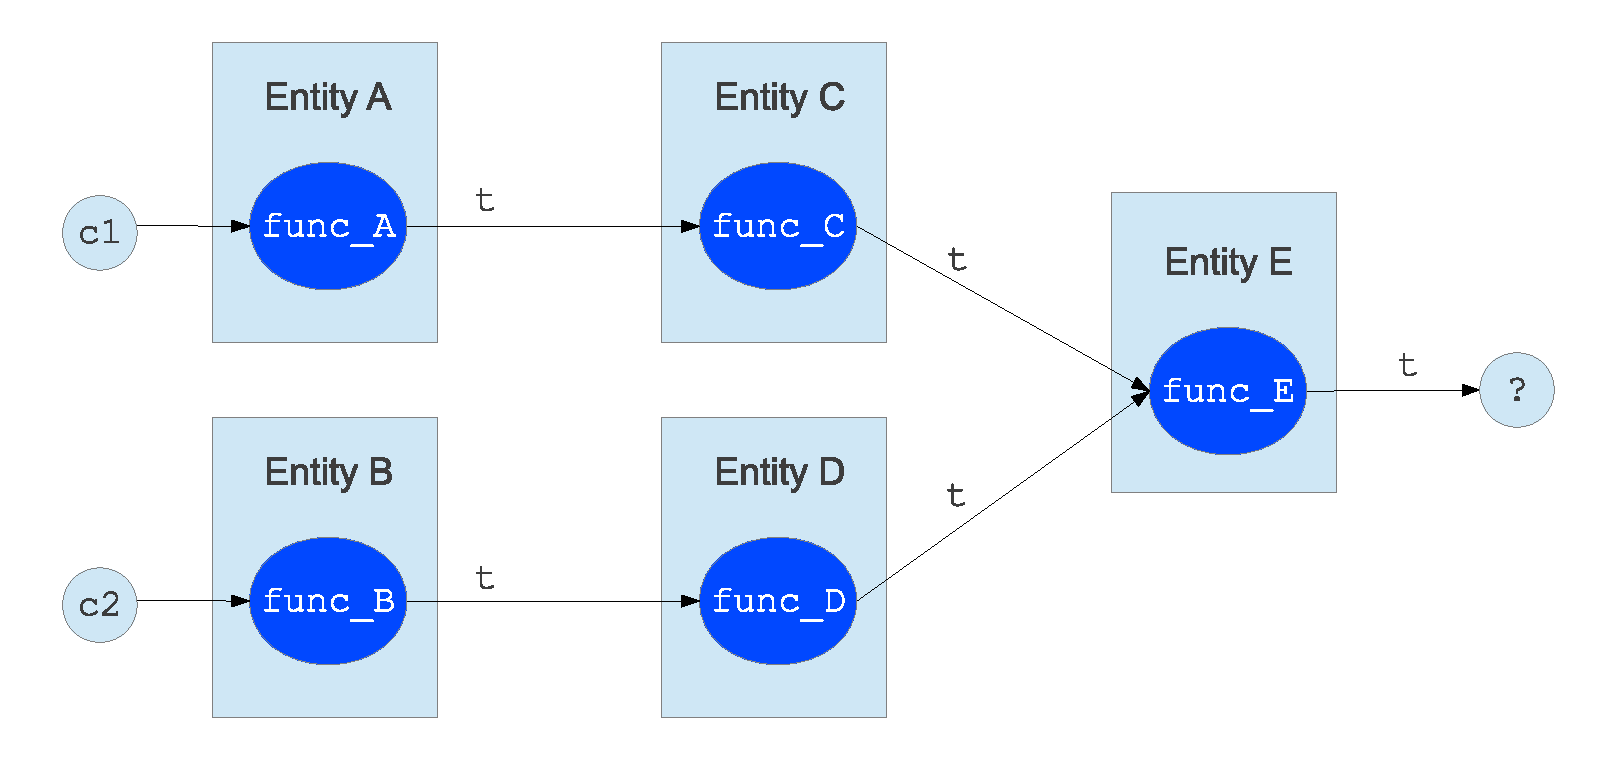
\includegraphics[width=0.8\textwidth]{../figures/dg.eps}
    \caption{Dynamic Graph with five entities $A-E$. Calculating the output of \texttt{Entity E} triggers a recursive backtracking until all entities are updated. In order to prevent an unnecessary recalculation of unchanged entities, signals are computed with a timestamp $t$. This timestamp keeps track of changes, which indicates whether an entity is outdated and has to be recomputed.}
    \label{fig:dg}
\end{figure}
\newpage
An example would be an entity called \textit{feature}, which calculates the error between the actual and desired position of the end-effector position. Thus, this entity comprises two input signals $p(t)$ and $p_{des}(t)$. The respective output signal provides the error, hence the name $e(t)$. The function linked to the output signal obviously computes the difference between $p$ and $p_{des}$ at time $t_i$. Algorithm \ref{algo:feature} describes this simple function, where the two input signals are fetched at the same timestamp and the resulting error is computed. The output signal equals the return value of the function.

\begin{algorithm}[]
\SetAlgoLined
\SetKwInOut{Input}{input}
\SetKwInOut{Output}{output}
\SetKwFunction{getp}{p\_signal\_in}
\SetKwFunction{getpdes}{p\_des\_signal\_in}
/* signals have to be initialized before */ \\
\Input{Timestamp $t$}
\Output{Error $e$}
p = \getp{$t$} \;
p\_des = \getpdes{$t$} \;
e = p\_des - p \;
return e \;
\caption{error computation in entity feature}
\label{algo:feature}
\end{algorithm}

\newpage
\subsection{SoT Core}
As mentioned in the beginning of this chapter, the SoT (meaning the hierarchical solver in this case) is realized as an dedicated entity inside the DG. This entity provides functionalities to dynamically push and pop task entities. 

We described already in the theoretical part, how a task definition looks like. Since we minimize a QP in the form of 
\begin{eqnarray}
\vec{Ax -b} &\quad& \textit{generic form} \notag \\
\vec{J \dot{q} - \dot{e}} &\quad& \textit{inverse kinematic} \notag
\end{eqnarray}
We have to specify the Jacobian $\vec{J}$ as well as the residual $\dot{e}$, which represents \mbox{- in this case -} the error between actual and desired position. 
The interface for a task implementation thus provides two output signals for the Jacobian and the error, respectively. 

In the previous section, we explained how output signals are handled inside the dynamic graph. The assigned output function for each signal is task dependent. An example positioning task for an end-effector can then easily be formulated by using the error calculation of the feature entity (see algorithm \ref{algo:feature}) and the Jacobian for the end-effector. 

We have to point out that at this point, we have only designed a task. We are not solving this task though. The task becomes part of the solver by explicitly pushing it onto the stack. The hierarchical solver in itself describes another entity, which holds all tasks, currently pushed on the stack. This entity solves the stack by fetching all \texttt{jacobian} and \texttt{error} output signals from all tasks. This will be transformed into one big, hierarchy respecting Jacobian and error. This will be finally solved and the result is provided as an output signal. We are not going any deeper into details here. The main information should be the requirements for designing tasks and push them on the stack for getting considered by the solver. Mathematical details can be found in \cite{escande-icra-10}\cite{escande:ijrr:2014}. An deeper insight into the development of the framework is provided in \cite{mansard-tro-09}.

Furthermore, we want to remind that the mathematical solver indeed solves the generic form of the above stated formulations. This being said, there is no need to specify $\vec{A}$ exclusively as a Jacobian matrix. This allows us also to specify tasks directly in joint space. 
\begin{eqnarray}
\vec{Ax -b} &\quad& \textit{generic form} \notag \\
\vec{I \dot{q} - \dot{q}_d} &\quad& \textit{joint space task} \notag
\end{eqnarray}
Where $\vec{I}$ denotes an identity matrix. The residual therefore has to be given in joint space, hence the naming $\vec{q_d}$, which specifies a desired joint velocity.

\section{Fast Collision Library (FCL)}
FCL is a fully templated library for generic collision detection and proximity calculations \cite{conf/icra/PanCM12}. It is designed to allow hierarchical proximity queries on various collision types among others such as axis-aligned bounding box (AABB), oriented bounding box (OBB) and swept sphere volume (SSV). It provides implementations based on Gilbert-Johnson-Keerthi (GJK) \cite{VandenBergen:1999:FRG:334709.334711} \cite{gjkoriginal} algorithms for proximity as well as collision detection for many geometry primitives such as boxes, cubes and spheres. 

Among them, a concrete capsule proximity implementation was not available during the time of this development. Based on the fact, that FCL is completely open source and developed with the standard template library (STL), it was possible to integrate the capsule decomposition into FCL. The work presented in chapter \ref{capsulecapsule} is at the time of writing integrated in FCL and can be obtained on github\footnote{\url{https://github.com/flexible-collision-library/fcl}}. 

The use of FCL as the main proximity library allows us to not exclusively focus on a hard-coded capsule decomposition. This being said, the same code can be used for example when certain body parts are wrapped with cubes as collision geometries. Contrary, as FCL is part of the core inside frameworks such as MoveIt!, the same capsule decomposition can be used for other applications. 
		
		\chapter{Collision Avoidance Implementation}\label{chapter:collisionavoidanceimpl}
In chapter \ref{chapter:collisionavoidance}, we analyze the theoretical aspects of our approach for collision avoidance. We examine in section \ref{sec:closestpoints} how a capsule decomposition and the according closest points between two capsules are sufficiently convex enough to cover the robots collision model. Additionally, we introduce a velocity damping method in \ref{sec:velocitydamping}, which restricts any positive velocity component along the directional vector towards the possible collision center. 

In the previous chapter \ref{chapter:implenv}, we briefly introduced the SoT as a framework and FCL as the according library for proximity queries. This chapter furnishes insights about the implementation of the closest point calculation and velocity damping as entities inside the DG.

Although it can be seen that those two components alone perform well to protect any (self-)collision, in practice there is a need for additional components. There are components needed to operate the robot with a smooth transition of movements. We additionally introduce task definitions for joint velocity and joint position limits as well as a weighting task, which can be used to operate the robot with the necessary safety.

In the following, we have to carefully differentiate the wording between an \textit{entity} and a \textit{task}. Technically speaking, a task denotes an entity inside the DG. Contrary, an entity is not a task, thus it is not able to be pushed on the stack and be considered by the solver.
\newpage
\section{FCL Entity}
As the name might reveal, the FCL entity is responsible for querying proximities based on FCL. We mentioned in the previous section, that during the development of this work, we enhanced FCL with the capsule capabilities. Thus, on startup, we load the capsule parameters such as origin, length and radius from a robot description file\footnote{Unified Robot Description Format(URDF), see \url{http://wiki.ros.org/urdf}}. This parses theses information into a capsule collision object and provides a full collision matrix of all given capsules. 

The collision matrix is represented by output signals for each collision pair. Each output signal provides the closest point from one capsule to another. Hereby, the signals are ordered according to the naming convention \texttt{<capsule-link-1><capsule-link-2>}, which indicates the closest point on the first capsule towards the closest point on the second capsule. Table \ref{tab:collisionmatrix} gives an example for three capsules, namely the right arm, the left arm and the torso. The table shows the resulting output signals. Inside the concrete application, the names are according to the names given in the robot description file.

\begin{table}[width=\textwidth]
\def\arraystretch{3}
\centering
\begin{tabular}{c|c|c|c}
					& 	right-capsule & left-capsule & torso-capsule \\
					\hline
right-capsule & X	& \pbox{4cm}{\texttt{<right-capsule}\\\texttt{left-capsule>}} & \pbox{4cm}{\texttt{<right-capsule}\\\texttt{torso-capsule>}} \\
\hline
left-capsule & \pbox{4cm}{\texttt{<left-capsule}\\ \texttt{right-capsule>}} & X & \pbox{4cm}{\texttt{<left-capsule}\\\texttt{torso-capsule>}} \\
\hline
torso-capsule & \pbox{4cm}{\texttt{<torso-capsule}\\\texttt{right-capsule>}} & \pbox{4cm}{\texttt{<torso-capsule}\\\texttt{left-capsule>}} & X 
\end{tabular}
\label{tab:collisionmatrix}
\caption{Collision Matrix and the produced output signal names.}
\end{table}

This full feature collision matrix might become relatively large, depending on the amount of capsules. This might lead to a large computational cost. At this point however, we only provide output signals inside the DG. With this in mind, the actual proximity computation only gets triggered, when an update of the respective signal is requested by another entity. 
\newpage
\section{Velocity Damping Task}
The implementation of the velocity damping inside a task follows after the FCL entity. We pointed out in the previous chapter \ref{chapter:implenv}, that for defining a task inside the stack, we have to implement a function for the \texttt{Jacobian} and \texttt{error} signal. For convenience, we repeat the inequality formulation of the velocity damping constraint in equation \ref{eqn:taskdampconstraint} here again. 
\begin{equation}
\vec{n}^T\vec{J(p_1,q)} \vec{\dot{q}} \geq - \epsilon \frac{d - ds}{\Delta t}
\end{equation}
In respect of the above equation, we implement the left hand side of the inequality inside the \texttt{Jacobian} function. The right hand side, the velocity boundary, is implemented in the \texttt{error} function. Moreover, we have to specify a set of parameters as input. The equation requires explicitly $\vec{p_1}$, $d_s$ and $\epsilon$ as given, implicitly it also requires $p_2$ to be set for calculating the remaining values such as $d$ and $\vec{n}$.

We will see during the examination of the experiments in chapter \ref{chapter:experiments}, that $d_s$ and $\epsilon$ have to be set as constant input signals as they heavily depend on the robot setup. The two points $\vec{p_1, p_2}$ can be obtained from the FCL entity, as these points are exactly the closest point pair of two collision objects. The connection will be done by plugging the output signals of the FCL entity, into the $\vec{p_1, p_2}$ input signals of the velocity damping task. The Jacobian has to be calculated according to the current joint positions. Our implementation takes the Jacobian with respect to the link origin. This calculation is most often already implemented in various kinematic or dynamic libraries; also inside the SoT. In order to get a Jacobian with respect to the closest point, we apply a twist transformation as explained in section \ref{sec:jacobian}. 

The DG setup for the self-collision avoidance is illustrated in the following graphic \ref{fig:capsuledistance}.
\begin{figure}[h!]
  \centering
    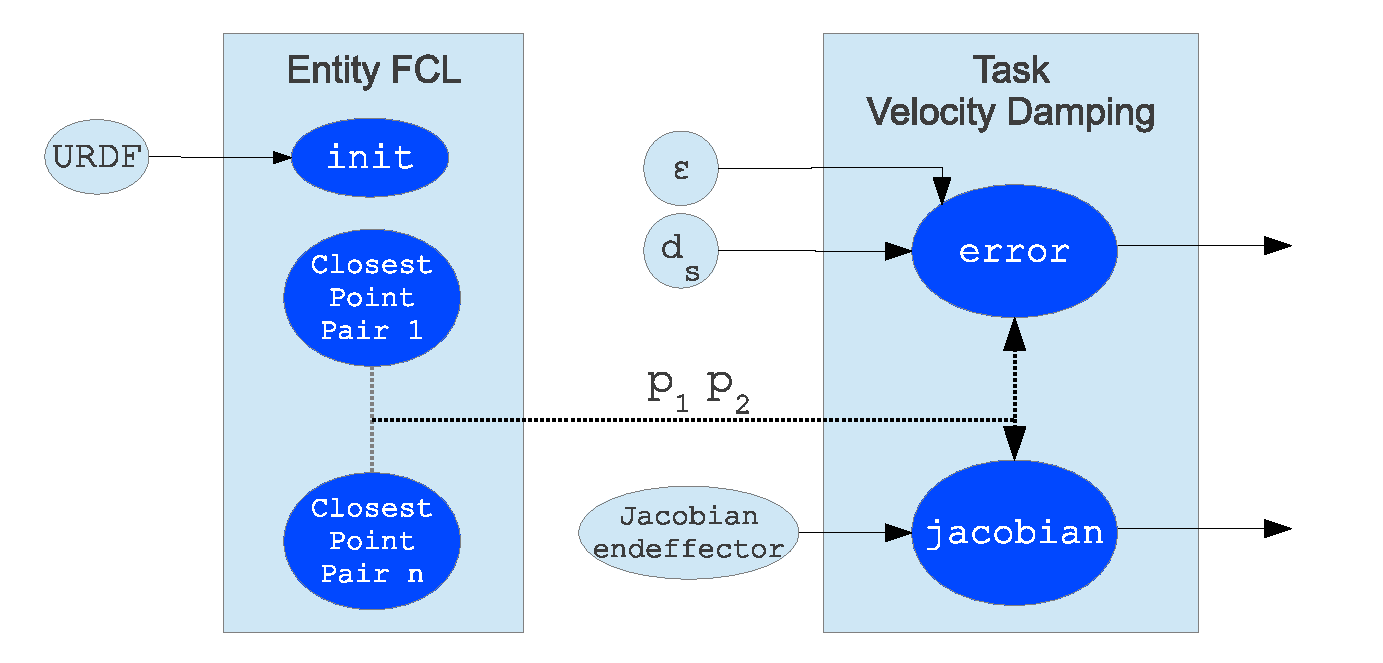
\includegraphics[width=0.8\textwidth]{../figures/dg_collision.eps}
    \caption{Dynamic Graph setup for the self-collision avoidance. EntityFCL provides the closest point pair calculation. These points are plugged into the velocity damping task for calculating $\vec{n}$ and $d$. Values such as $d_s$ and $\epsilon$ are provided as constant signals. Most kinematic or dynamic libraries provide already ways to compute a Jacobian with respect to the end-effector. We provide the end-effector Jacobian as an input signal and apply a twist operation in order to obtain the Jacobian with respect to the closest point. The output signals of the velocity damping are in accordance with the abstract task definition of the SoT, since it requires a \texttt{Jacobian} and \texttt{error} function.}
    \label{fig:capsuledistance}
\end{figure}

We execute only one velocity damping task for avoiding all possible self-collisions. This means, that all collision pairs are on the same level inside the hierarchy. Thus, we configure the task velocity damping to possess multiple input sockets for all closest point pairs and the according control parameters such as $d_s$ and $\epsilon$. This formulation treats all collisions with the same priority.

On the same hand, we only plug the collision pairs we really need to protect the complete robot. This implies an exclusion of adjacent body parts, since they are constantly in collision and would thus violate the solver during the complete execution time. Furthermore, we can exclude collision pairs, which are not able to collide based on the mechanical construction of the robot, such as left and right shoulder. This makes the configuration effort rather simple and the computational complexity is on a minimal.

\section{Joint Limits Task}
The two entities, we described previously, are capable of preventing any self-collision with the robot. However, if we execute only the velocity damping as an exclusive task, we run into trouble as the joint limits might get exceeded. This results in heavy discontinuities which might in the end even destroy the robot. For this purpose of protecting the motors and gears, we introduce two tasks in joint space, which take care about joint position exceeding as well as joint velocity limits. In the generic robot description file, we can calibrate persistent values for the minimal and maximal position for each joint. 

The hierarchical solver inside the SoT operates inside the velocity domain. Thus, for a positioning task, we have to specify a Jacobian matrix, which translates joint space velocities into cartesian space velocities. This formulation allows us to specify the error residual, for example the error between desired and actual position of an end-effector, in cartesian space. \\
At this point, we want to specify a joint space residual, namely the distance between the current joint position and the maximal or minimal boundary. In order to specify this in a similar way, we replace the Jacobian matrix by a simple identity matrix. The task definition then becomes the following:
\begin{equation}
\vec{I} \vec{\dot{q}} \geq \vec{\dot{q}_{err}} \quad \textit{with } \vec{\dot{q}},\vec{\dot{q_{err}}} \in \mathbb{R}^{1\times n}
\end{equation}
where $\vec{I}$ denotes the identity matrix and $\vec{\dot{q_{err}}}$ the error in joint velocity. We have to note here, that the error has to be given in the velocity domain, rather than position. This implies, we have to take the first derivative of the joint position error. Thus the above formulation turns into
\begin{equation}
\vec{I} \vec{\dot{q}} \leq \frac{\vec{q_{max}-q}}{\Delta t} \quad \textit{with } \vec{q_{max}},\vec{\dot{q}} \in \mathbb{R}^{1\times n}
\end{equation}
where $\vec{q_{max}}$ specifies the maximal joint position. $\Delta t$ denotes the time between two computation cycles, which we use to compute a first numerical derivative between two joint positions in time. We enhance this formulation with an additional control gain $k$ to ease any recalibration on runtime. The final equation formulation is presented in equation \ref{eqn:jointlimit}
\begin{eqnarray}\label{eqn:jointlimit}
\vec{I} \vec{\dot{q}} &\leq& \frac{\vec{q_{max}-q}}{k \Delta t}  \notag \\
\vec{I} \vec{\dot{q}} &\geq& \frac{\vec{q_{min}-q}}{k \Delta t}
\end{eqnarray}
We have to point out, that $k$ is placed in the denominator. This has the meaning, that an increase of $k$ leads to an decrease of maximal joint position changes. We implement the joint position limits as a double bounded task, restricting the joint position in the lower and upper boundary. 

The above formulation prevents the solver to resolve any joint state vector $\vec{q}$, which would exceed any joint positions. However, it does not take the joint velocity into considerations. Image equation \ref{eqn:jointlimit} with a low value for $k$ and a current joint position vector $\vec{q}$, which is in the middle of the position limits. There can be situations, where the resulting allowed velocity $\vec{\dot{q}}$ might be too high for the motors. On the same hand, restricting the velocity with a rather big value for $k$ also shrinks down low velocities.

Based on the above considerations, we implement a velocity clamping on top of it. Hereby, in the robot description file, we further specify a maximal joint velocity value. With this, we execute the joint limits with the above formulation, however check if the resulting boundary, the right hand side of the inequality, exceeds the maximal velocity. The task definition looks like the following:

\begin{eqnarray}
\vec{I} \vec{\dot{q}} &\leq& \left\{
\begin{array}{l l}
\frac{\vec{q_{max}-q}}{\Delta t}  & \text{ if } \vec{\dot{q_{err}}}\leq \vec{\dot{q}_{max}} \\
\vec{\dot{q}_{max}} & \text{else}
\end{array} \right. \notag \\
\vec{I} \vec{\dot{q}} &\geq& \left\{
\begin{array}{l l}
\frac{\vec{q_{min}-q}}{\Delta t}  & \text{ if } \vec{\dot{q_{err}}}\leq \vec{\dot{q}_{min}} \\
\vec{\dot{q}_{min}} & \text{else}
\end{array} \right.
\end{eqnarray}
\newpage
\section{Joint Weighting Task}
Finally, we introduce a task, which restricts the movement of expensive joints such as the torso. This task is not necessarily a requirement for safe operations with the robot. It is more a task, which limits the movement of heavy torques and inertia. It further improves the workspace of the robot, since a weighting of the torso means a lower movement of the most commonly shared part of the kinematic chain. The torso will be shared between the head and both arms. However, those tasks of positioning head and arms might be in different priority level such that the torso almost exclusively respects the highest of those tasks. We can correct this by weighting the torso, which is getting compensated by foster a larger movement of different joints, e.g. in the respective arms.

We can easily formulate this task again in joint space. In contrast to the pure identity matrix, we multiply a diagonal weighting matrix with entries according to the inertia of the robot. As we try to minimize the movement as much as possible, we set the resulting velocity to zero.  
\begin{equation}
\vec{W} \vec{I} \vec{\dot{q}} = 0 \quad \text{with } \vec{W} \in \mathbb{R}^{n \times n}
\end{equation}

The equation successfully limits the movement according to the value set on the main diagonal of the weighting matrix. However, when we look at this formulation inside the stack, this approach has some limitations. When we set this task as a rather high priority, the robot does not move. It is clear, that when this task will be fully solved, all DoF are getting used and there is no nullspace for lower priority tasks. With this in mind, we have to set this weighting task always at the least priority position, in order to minimize the velocities. The optimization is done according to the weights as much as possible, yet not restricting any other tasks.



		\chapter{Experiments}
\label{chapter:experiments}
The solution of this work was validated with a couple of experiments and stress tests. We show in the following, that this approach provides a safe way to avoid collisions with the robot itself as well as avoiding external obstacles. Reviewing the goal statements of the introduction \ref{item:goals}, we conducted the following experiments to get a quantitative evaluation:
\begin{itemize}
	\item Providing a piecewise continuous trajectory of closest point pairs
	\item Avoiding collisions between the actuated hand and external obstacles
	\item Avoiding full self-collision 
\end{itemize}

\section{Robot Hardware Setup}
The conducted experiments have been mainly examined with a real time physics simulator, namely Gazebo. It simulates an appropriate robot behavior in terms of joint position as well as joint velocities.

The full body self-collision avoidance is running successfully on the robot. This being said, this chapter briefly introduces the hardware on the robot (REEM-H in this case) to give the reader an overview over the experiment circumstances. 

REEM-H comprises an embedded computer, running a Ubuntu 12.04 LTS version with a real time kernel. The specifications as they are provided on PAL Robotics website at the time of writing are listed in table \ref{tab:reemhspec}. 

Furthermore, the used robot model is presented below. The three images denote the internals of the robot (figure \ref{fig:reemmodels}). In the first image, we can see the visual model of REEM-H. The kinematic chain is illustrated in the second image. Hereby, the names of the used links are shown as well \footnote{For completeness: We omitted arm\_link\_6 on both arms as they are located in the same position than the tool link. The graphic looks clearer this way and link\_6 carries no necessary need in terms of capsule decomposition.}. In the remainder of this chapter, we may refer to them, as we calculate the closest point pair based on those links. Finally, the third image gives an idea about the undertaken capsule decomposition. 

\begin{figure}[h!]
  \centering
  \subfigure[REEM-H Model]{
  		\label{fig:reemmodel} 
  		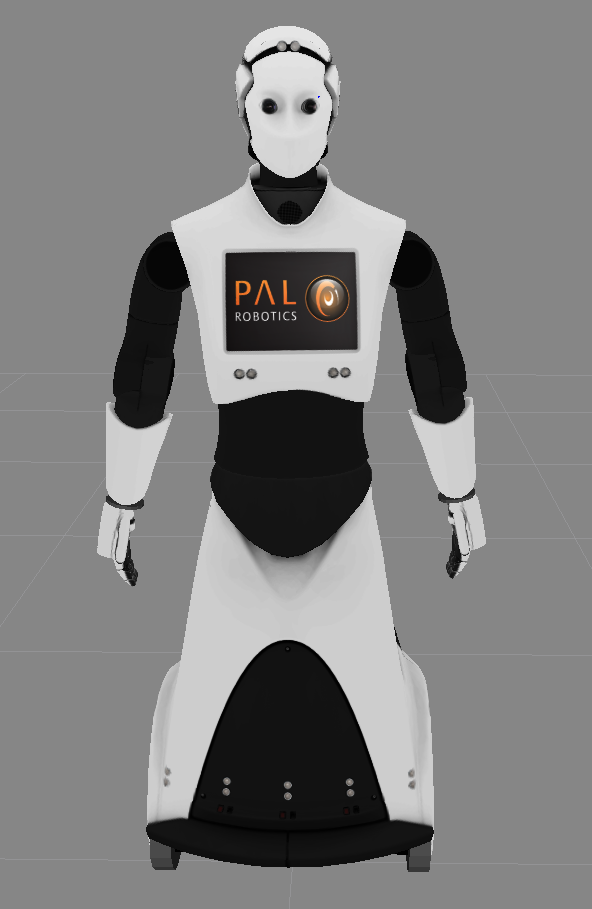
\includegraphics[width=0.3\textwidth]{../figures/reem_model.png}
  	}
  	  \subfigure[Kinematic Chains]{
  		\label{fig:reemtf} 
  		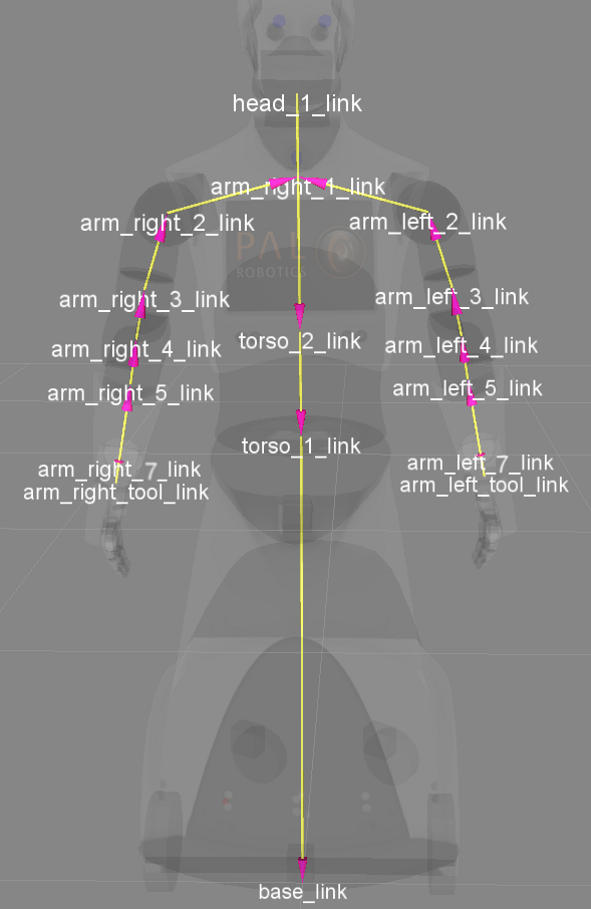
\includegraphics[width=0.3\textwidth]{../figures/reem_model_tf.png}
  	}
  	  \subfigure[Capsule Decomposition]{
  		\label{fig:reemcaps} 
  		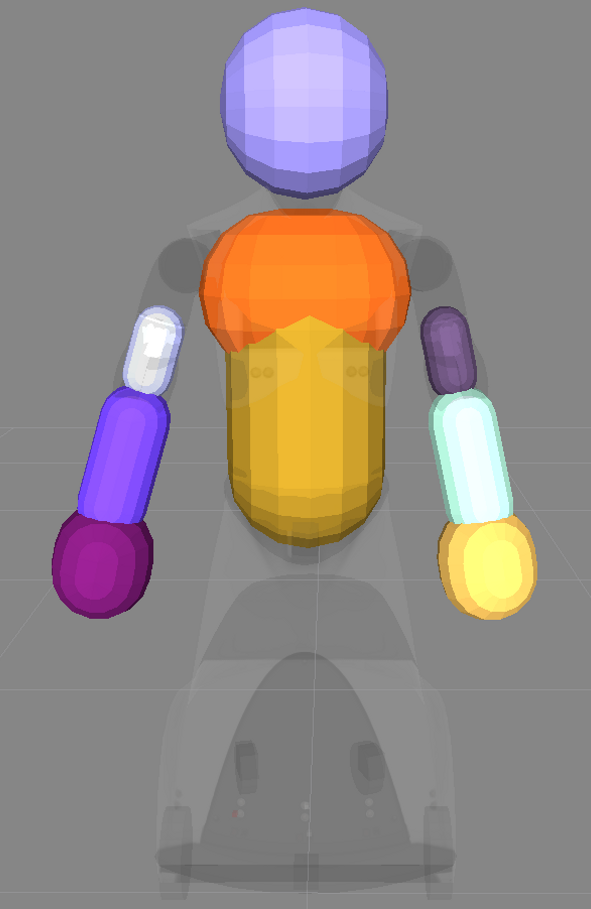
\includegraphics[width=0.3\textwidth]{../figures/reem_model_capsule.png}
  	}
\caption{REEM-H model explained: a) visual surface model. b) kinematic chain of all links. These link names are used as a reference in the remainder of this chapter. c) implemented capsule decomposition. Three capsules are placed on each arm, two on the upper body as well as one for the head.}
    \label{fig:reemmodels}
\end{figure}
During the development of this work, we could determine the shown capsules in figure \ref{fig:reemcaps} as being sufficiently necessary to protect all possible self-collisions. 
Since we are implementing a safety distance threshold on every capsule, the resulting safety padding of all capsules sufficiently covers the left out body parts. Table \ref{tab:capsules} lists the capsule decomposition of the body parts.
\begin{table}[h!]
\parbox{.45\textwidth}{
\begin{tabular}{l l} 
\hline
\multicolumn{2}{ |c| }{REEM-H specification} \\
\hline
weight & 90 KG \\[0.2em]
\hline
height & 1.70 meter \\[0.2em]
\hline
DOF & 22 \\[0.2em]
\hline
Computer & Intel Core2Duo \\[0.2em]
\hline
OS & Ubuntu 12.04 LTS \\[0.2em]
\hline
Kenel & Xenomai real time toolchain\\
\end{tabular}
\caption{Hardware specification of REEM-H}
}\label{tab:reemhspec}
\hfill
\parbox{.45\textwidth}{
\label{tab:capsules} 
\begin{tabular}{l l}
\hline 
\multicolumn{2}{ |c| }{Capsule Decomposition} \\
\hline
\multirow{3}{*}{Right Arm} & arm\_right\_3\_link \\
& arm\_right\_5\_link \\
& arm\_right\_7\_link \\[0.2em]
\hline
\multirow{3}{*}{Left Arm} & arm\_left\_3\_link \\
& arm\_left\_5\_link \\
& arm\_left\_7\_link \\[0.2em]
\hline 
\multirow{2}{*}{Upper Body} & torso\_1\_link \\
& torso\_2\_link \\[0.2em]
\hline
\multirow{1}{*}{Head} & head\_1\_link \\
\end{tabular}
\caption{Capsule Decomposition of REEM-H}
}
\end{table}

\section{Experiments}
All of the following concrete experiments comprise two major tasks. The highest prioritized task of all experiments is joint limit avoidance. This is followed by the task velocity damping introduced in chapter \ref{sec:velocitydamping}, which denotes the (self-)collision avoidance task. Hereby, this is configured according to the respective exercise (such as external collision avoidance or self-collision avoidance). Lastly, the active task for positioning the tool center of the left as well as the right arm is placed at the bottom of the stack. Figure \ref{fig:basicstack} depicts the basic stack used for these experiments. During the experiments, we change the order of the left and right wrist, however they are constantly placed at the bottom of the task.
\begin{figure}[h!]
  \centering
    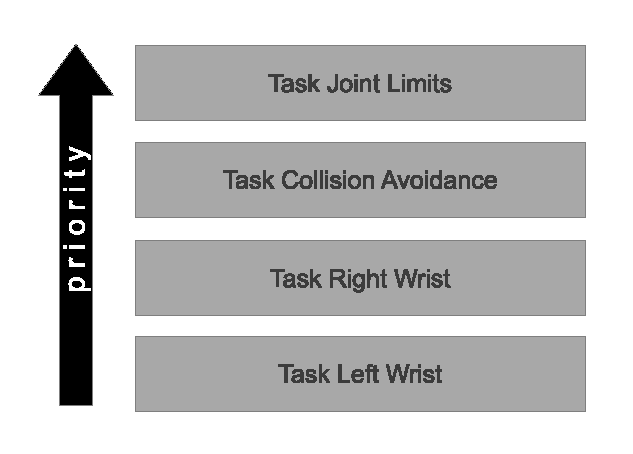
\includegraphics[width=0.4\textwidth]{../figures/stack_experiments.eps}
    \caption{Basic hierarchy stack of used tasks for the experiments. As illustrated, joint limits have always the highest priority. The collision avoidance task takes precedence over the tasks of interest such as the right or left wrist. In the conducted experiments, we will also examine the behavior of changing the order of left and right, yet constantly placing them at least priority.}
    \label{fig:basicstack}
\end{figure}

Beforehand, we implemented two strategies for integrating the SoT inside ROS\_control of the REEM robots. Xenomai respectively ROS\_control operates with a frequency of $100Hz$. This means, that the physical update cycle is lower bounded to $100Hz$ and the computation of the stack has to produce a result with in this cycle. On the same hand, we integrated the SoT as a asynchronous, not real time safe thread, next to ROS\_control. With this decoupling, we can prevent any real time violations to be visible on the robot. This further implies, that we can achieve a higher cycle rate exclusively for the SoT, providing the current solution for every cycle of ROS\_control. 
The purpose of these different cycle rates is essentially the capability of shrinking the $\Delta t$ inside the update cycle of the SoT. We recall the task definition in \ref{eqn:ikleastsquare} again:
\begin{eqnarray}
\vec{\dot{x} = J(q,t) \dot{q}} \notag \\
\vec{\dot{x} = J(q,p)} \frac{\Delta\vec{q}}{\Delta t} \label{eqn:expdeltat}
\end{eqnarray}
From equation \ref{eqn:expdeltat}, it is clear that lowering $\Delta t$ yields to smoother results in $\vec{\dot{x}}$ and thus to a smoother trajectory on the robot. All experiments, which are presented below, were executed with a rate of $100Hz$ inside the SoT, because of limits in computation power of the embedded computer inside REEM.

\subsection{Continuous Trajectory of Closest Points}
In chapter \ref{sec:closestpoints}, we examined the benefit of exercising a capsule decomposition over a mesh collision geometry. The goal in this experiment is to demonstrate the required continuity of the closest point pair. Informally spoken, monitoring the trajectory of each point of the according point pair must result in one single path and is not allowed to jump in position. 

For this experiment, we move the right arm from the right ($x:-0.2m,y:-0.3m,z:1.1m$) to the left($x:0.2m,y:0.3m,z:1.1m$). Hereby, we examine the development of the closest point pair between arm\_right\_5\_link and the Upper Body as well as Head. The arm movement as well as the closest point calculation is shown in the two figures below (figure \ref{fig:cpexperiment}). Figure \ref{fig:cplines} contains information about the closest point pairs at time $t_k$ for a specific $k$. The lines mark the connection between the two points which form a collision pair. 

\begin{figure}[h!]
  \centering
  \subfigure[Executed trajectory]{
  		\label{fig:cptraj} 
  		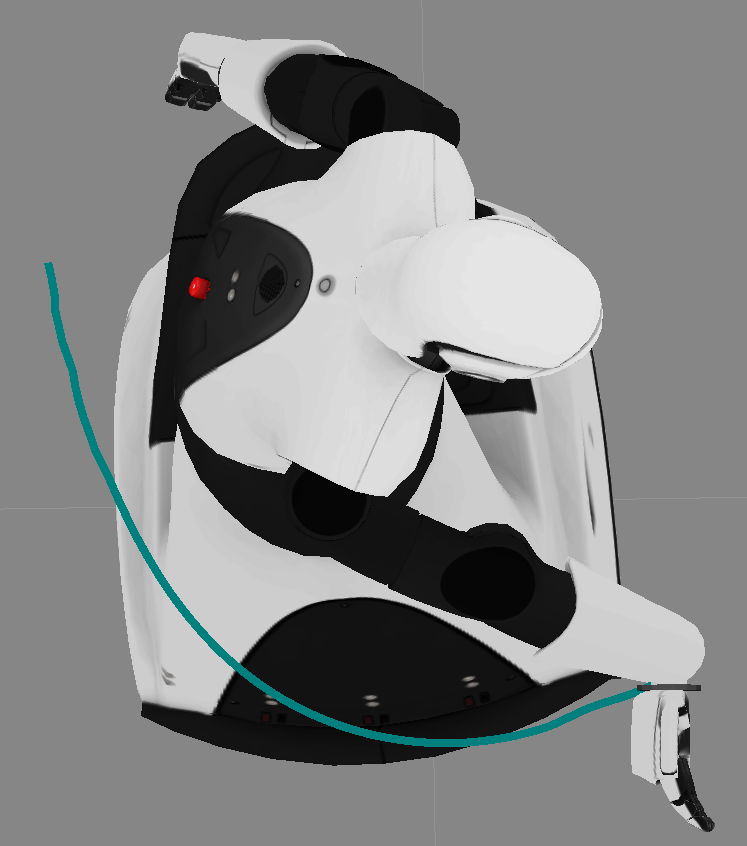
\includegraphics[width=0.35\textwidth]{../figures/closest_points/robot_path.png}
  	}
  	  \subfigure[Closest Point Pairs]{
  		\label{fig:cplines} 
  		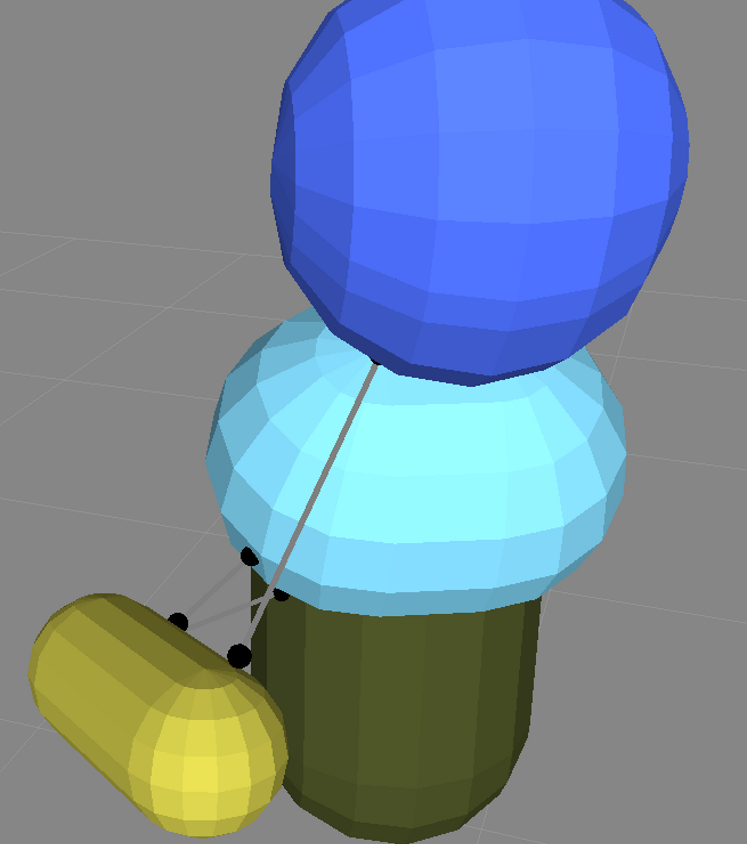
\includegraphics[width=0.35\textwidth]{../figures/closest_points/lines.png}
  	}
\caption{Closest Point Trajectory: a) shows the trajectory the right arm executed. The robot moved around the torso from the right ($x:-0.2m,y:-0.3m,z:1.1m$) to the left($x:0.2m,y:0.3m,z:1.1m$) (seen from the robot perspective). b) denotes the closest point pairs between the three collision pairs at $t_k$. The development of this calculation has to be continuous for all $t_i$. The lines are providing info which points belong to which collision pair.  } 
    \label{fig:cpexperiment}
\end{figure}

The result of this particular experiment is exposed below. We can see in the results (figure \ref{fig:cptogether}), that the requirement is fulfilled as the trajectory for all closest points is continuous. The plots show the path in $x$ and $y$, since the executed movement is planer in $z:1.1m$. The left plot describes the points, which are attached at the \verb|arm_right_5_link|. Their data is expressed with respect to the global base frame. Equally, the right plot represents the points on the Upper Body and Head.
%\begin{figure}[h!]
%  \centering
%  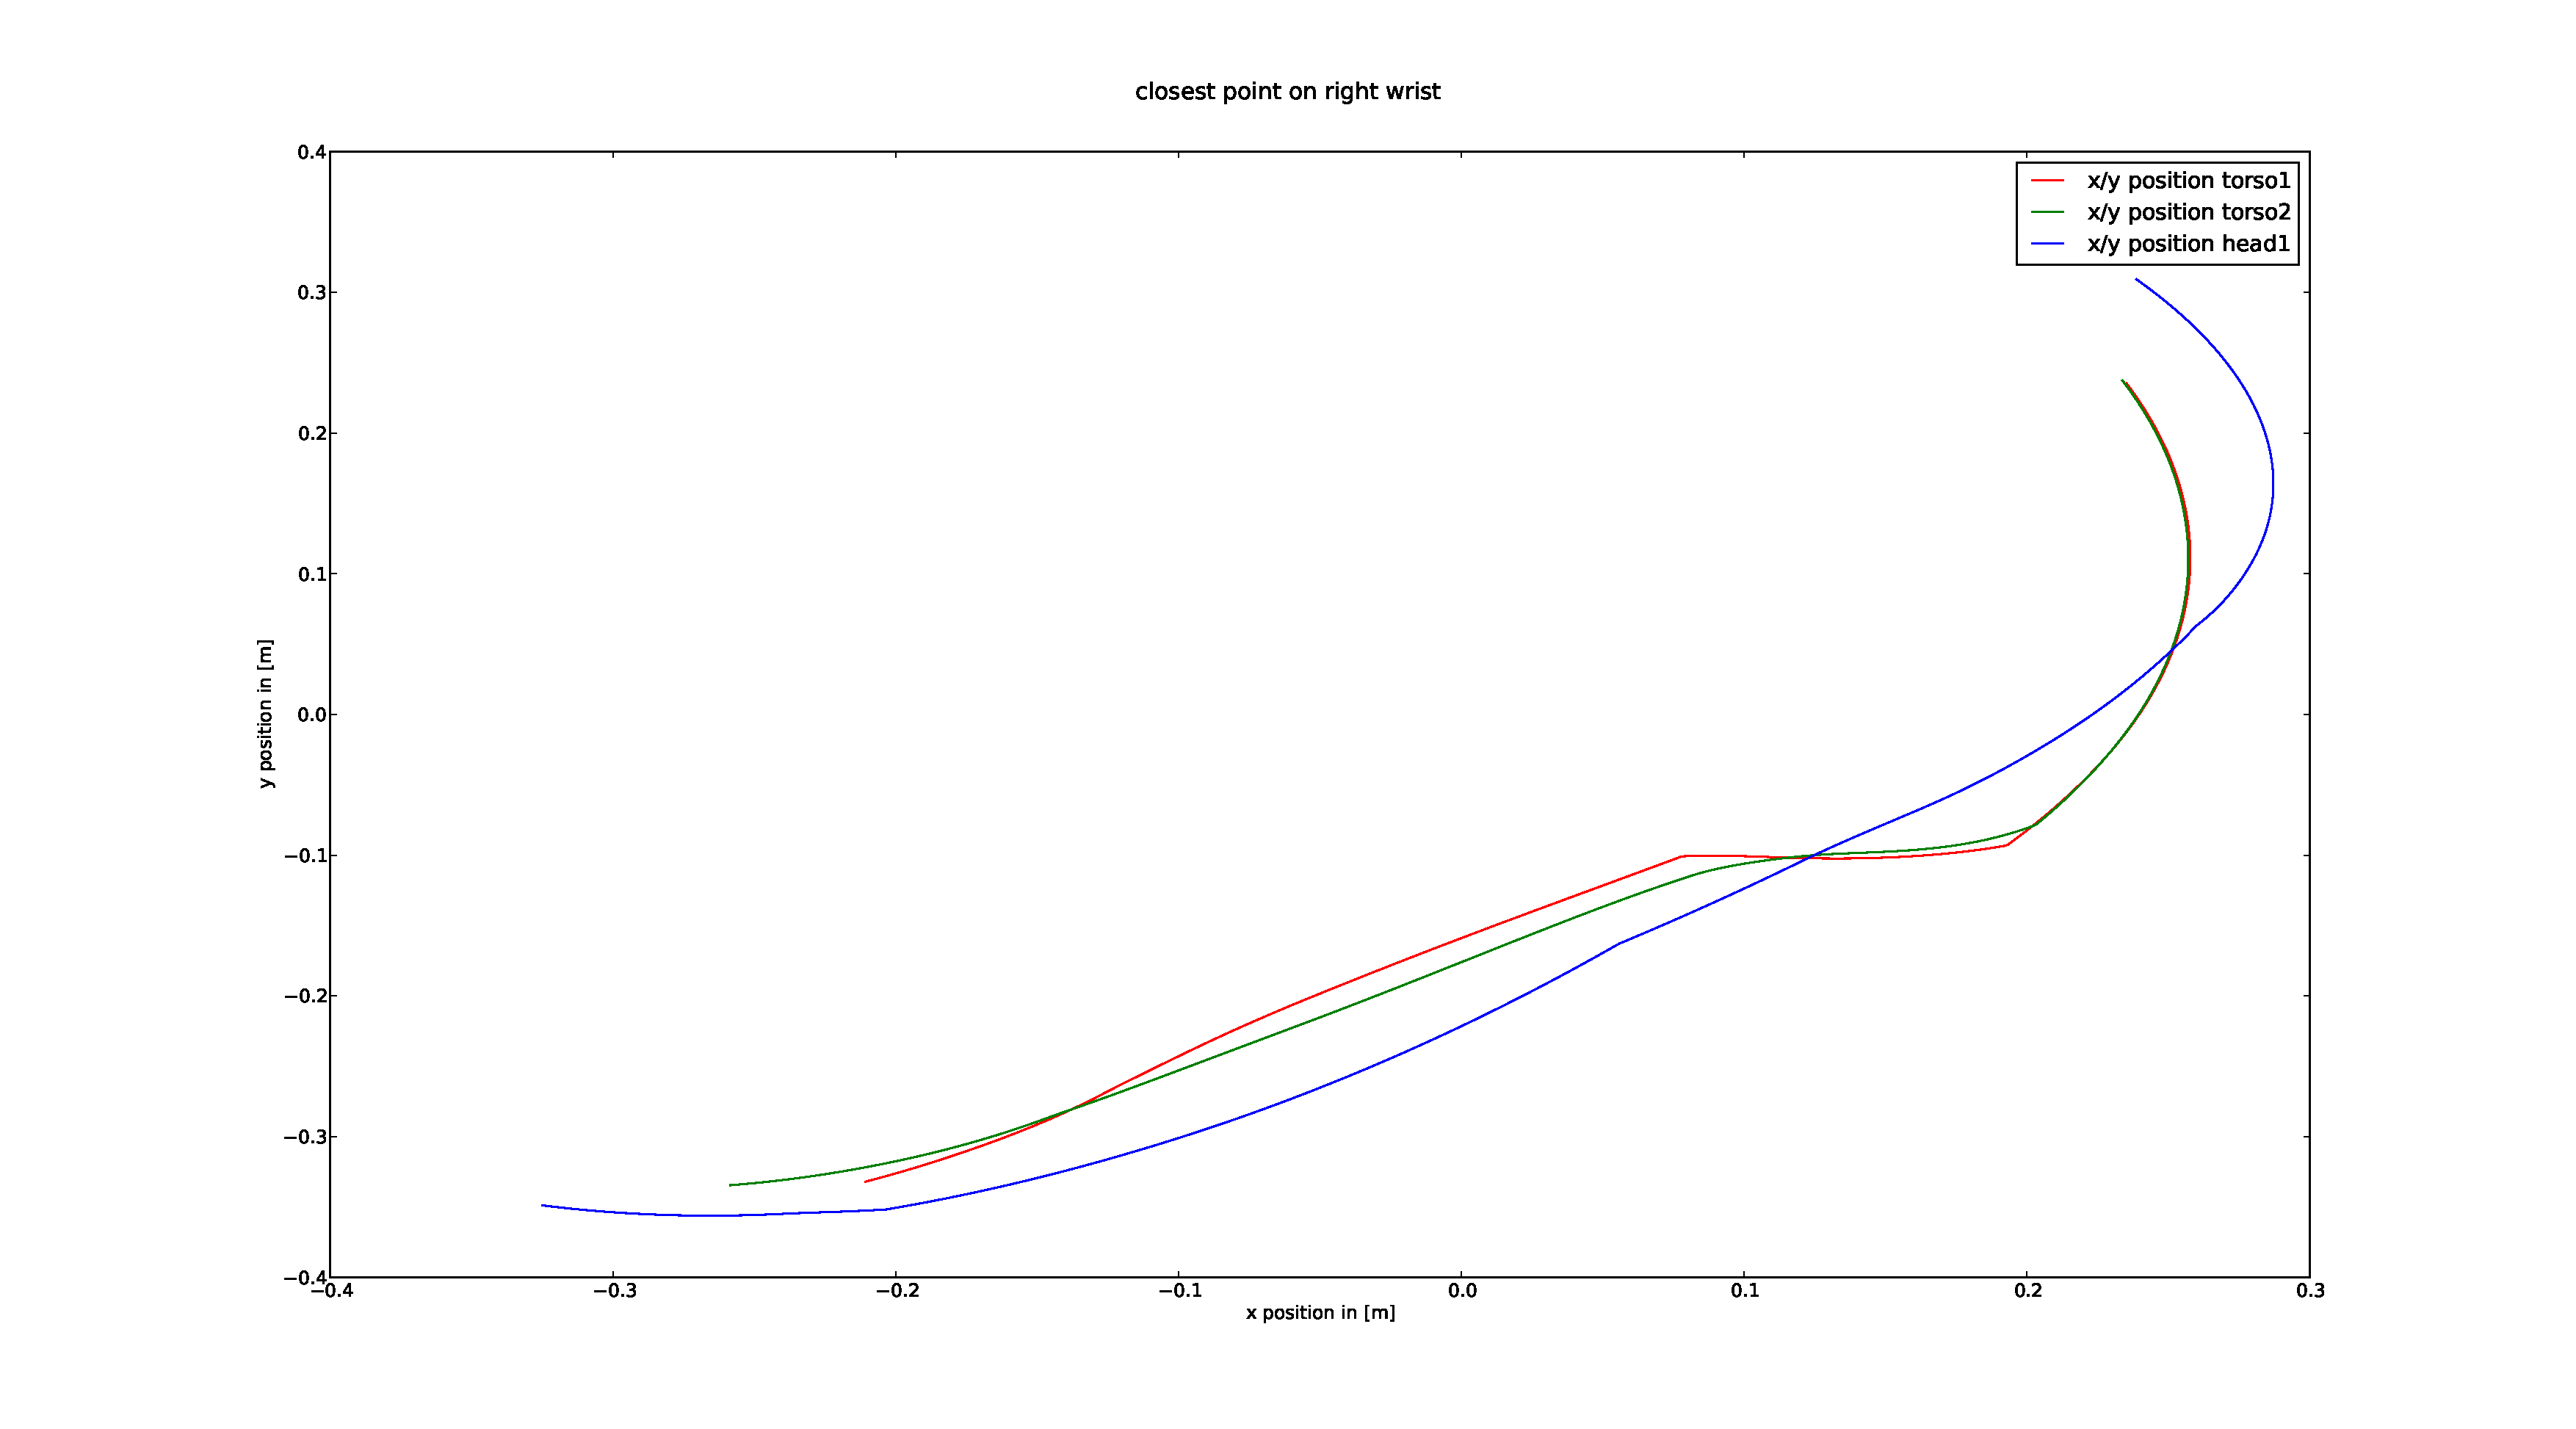
\includegraphics[width=0.9\textwidth]{../figures/closest_points/three_topics_rw.eps}
%\caption{closest point development of the points lying on \texttt{arm\_right\_5\_link}. The result is a continuous path, which illustrates a correct behavior of the calculation.} 
%    \label{fig:cprw}
%\end{figure}
%\begin{figure}[h!]
%  \centering
%  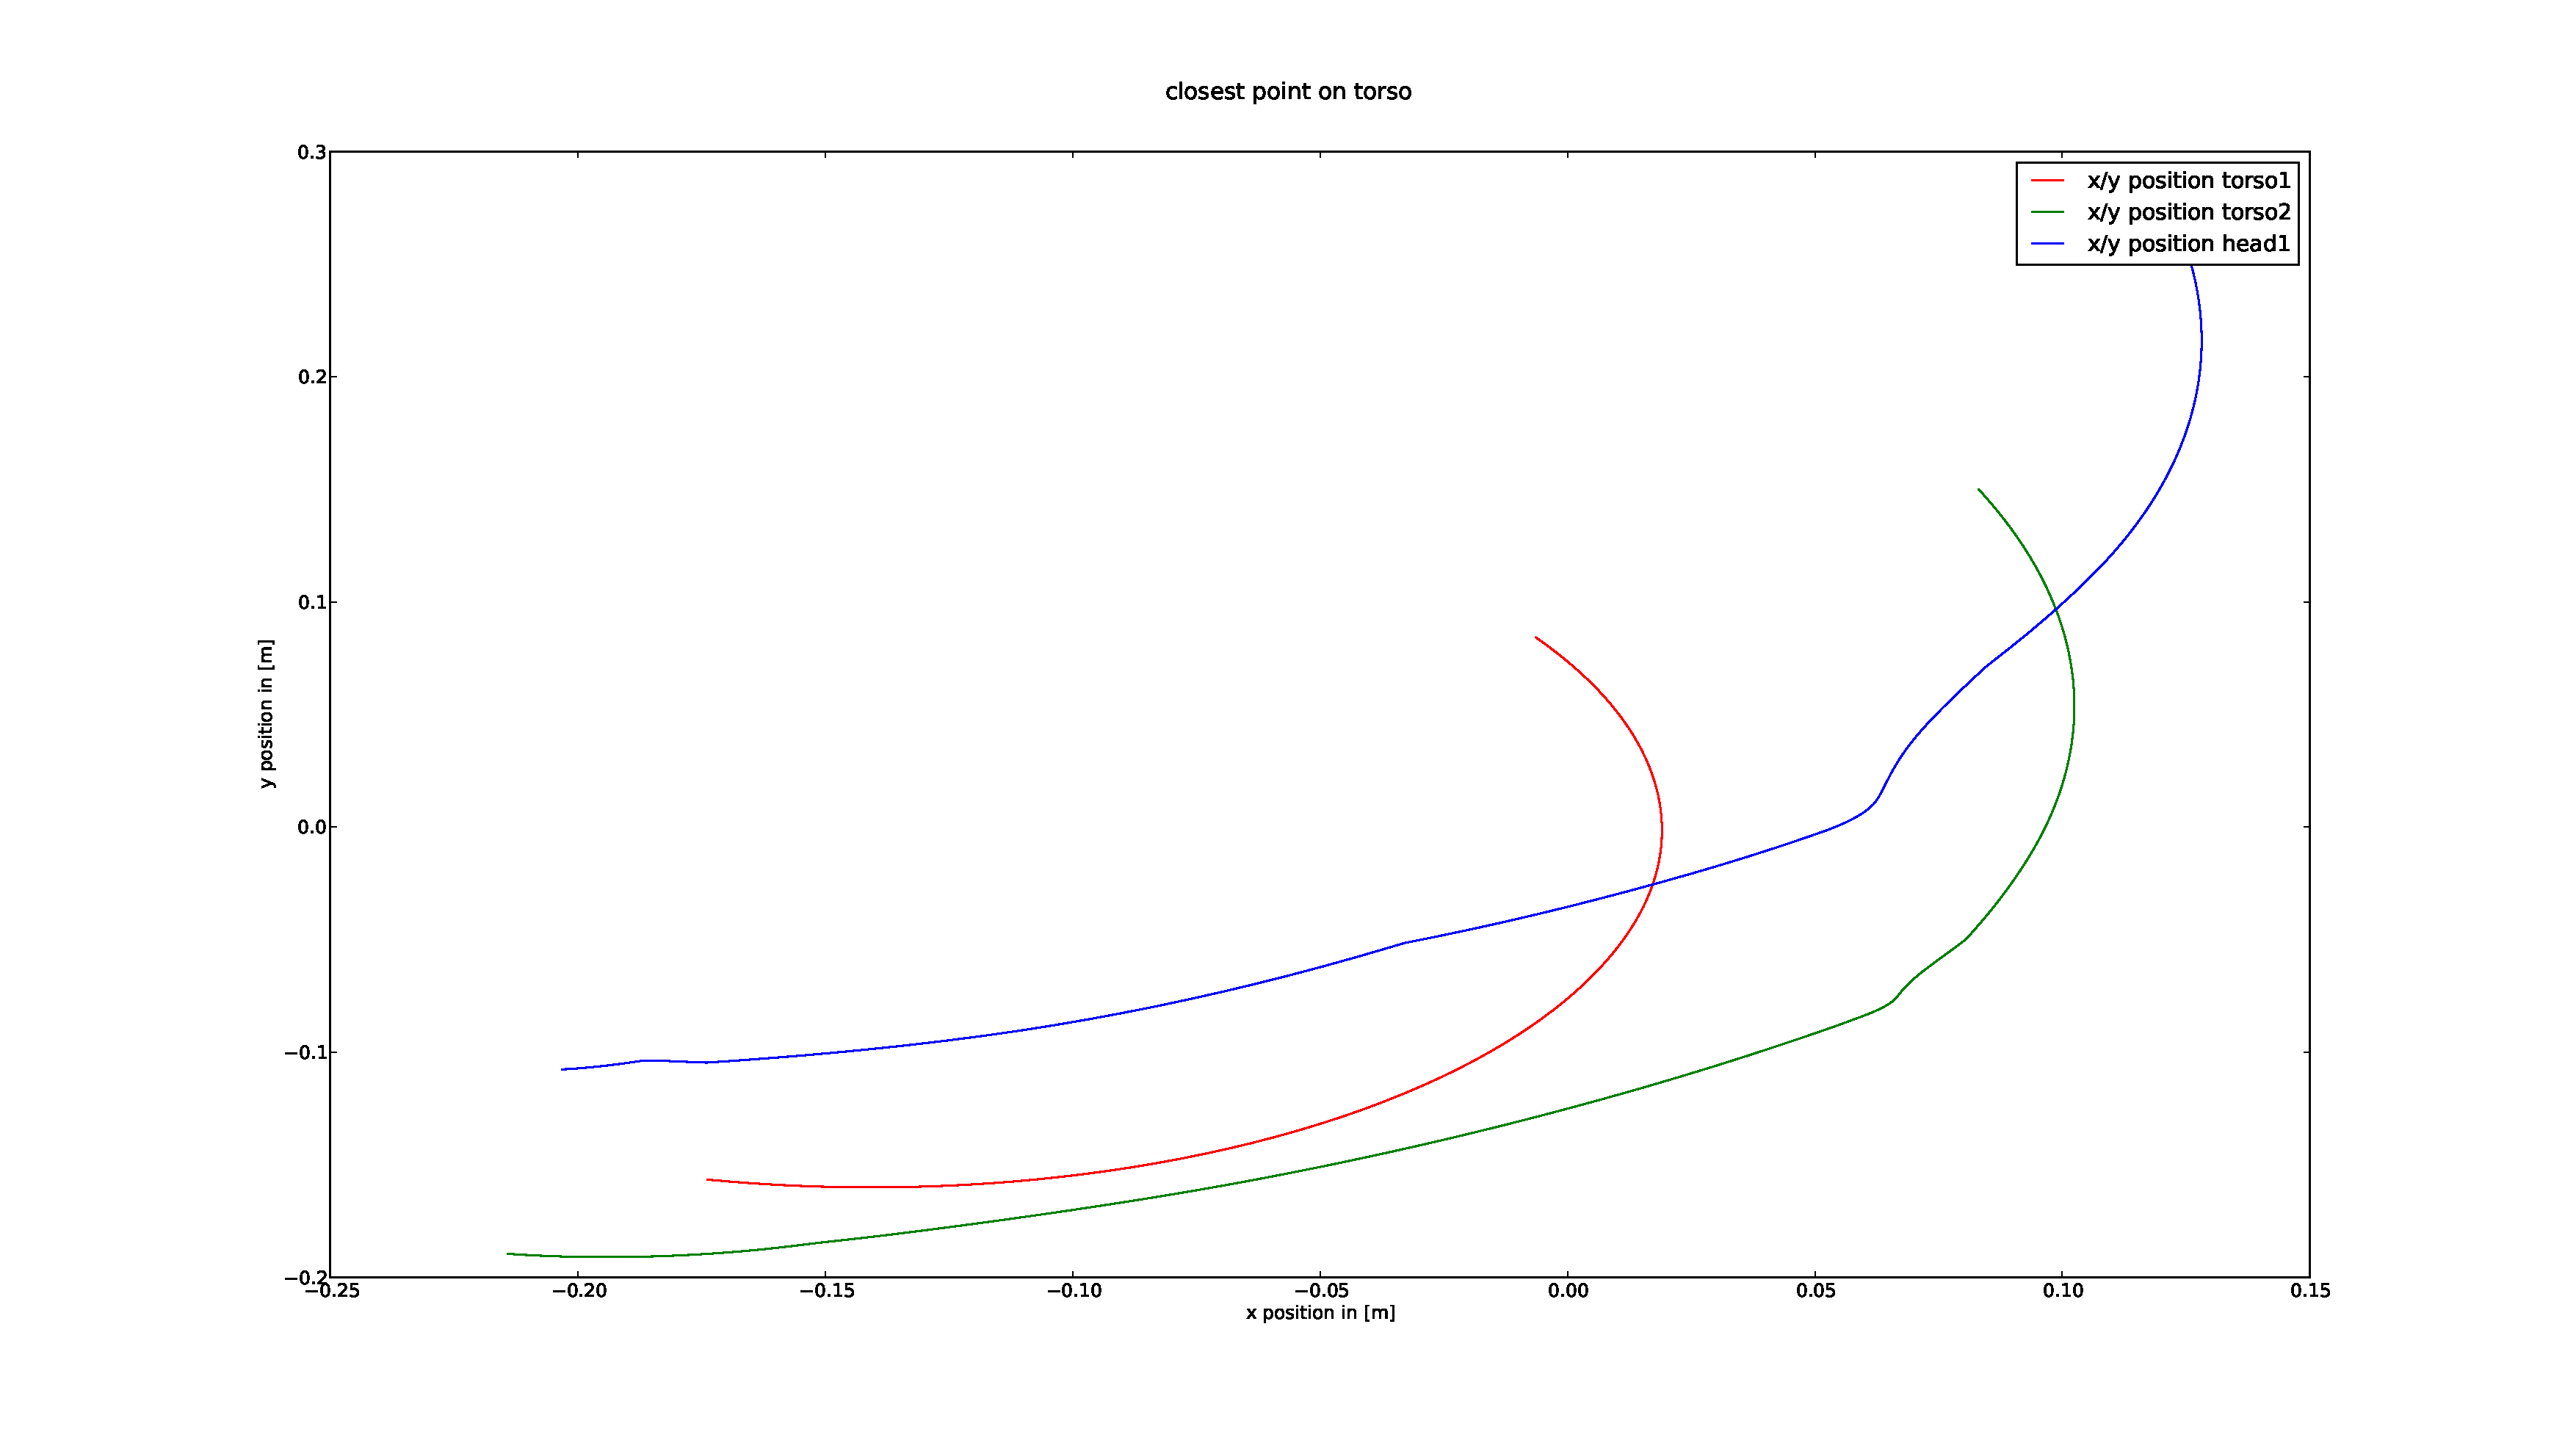
\includegraphics[width=0.9\textwidth]{../figures/closest_points/three_topics_torso.eps}
%\caption{closest point development of the points lying on Upper Body and Head, respectively. The result is also continuous path, which illustrates a correct behavior of the calculation.} 
%    \label{fig:cptorso}
%\end{figure}
\begin{figure}[h!]
  %\centering
  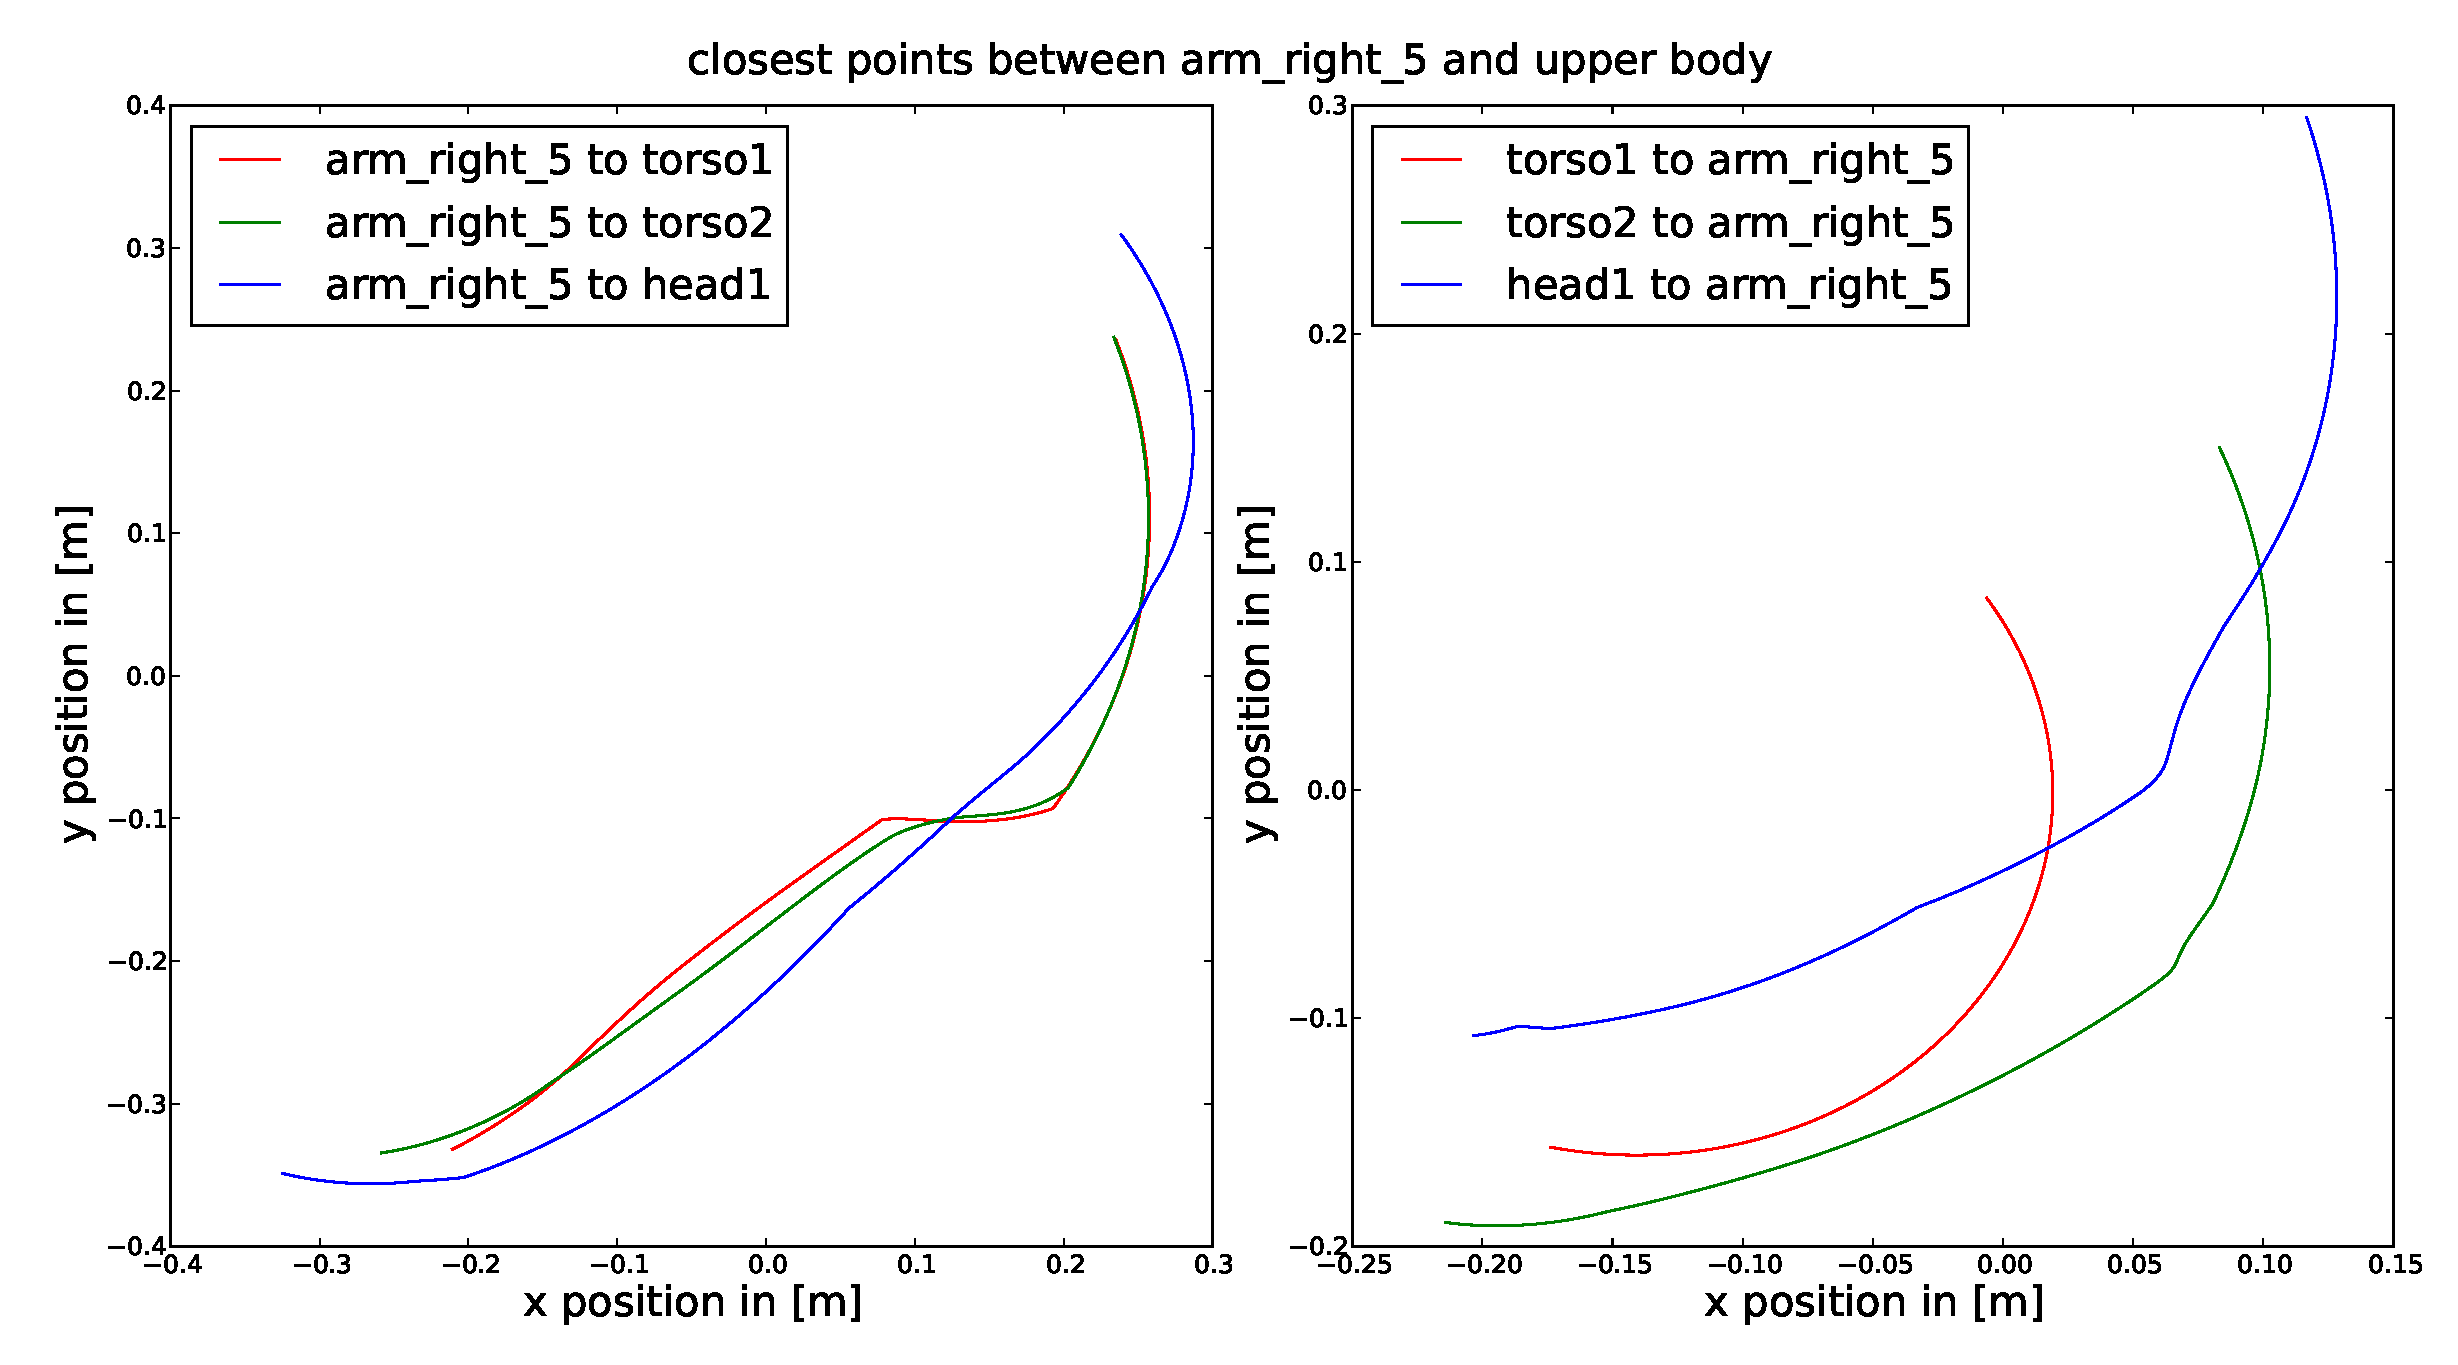
\includegraphics[width=\textwidth]{../figures/closest_points/three_topics_together.eps}
\caption{closest point development between \texttt{arm\_right\_5\_link} and Upper Body (consisting of \texttt{torso\_1, torso\_2, head\_1}). Left diagram shows the closest points lying on the capsule of the right arm towards the upper body. Similarly, the right diagrams displays the counter points on the upper body, which are pointing towards the right arm. } 
    \label{fig:cptogether}
\end{figure}

This experiment was successfully executed with all possible collision pairs with similar results. We encounter a rather negative result, when joint limits or clamping situations occur as the resulting joint velocities might increase dramatically. This inevitably leads to a high displacement of the closest points.
\clearpage
\newpage
\newpage
\subsection{External Collision Avoidance}
To begin with, we conduct the experiment of avoiding external obstacles coming across a predefined trajectory of one of the arms. Hereby, we specify a trajectory input signal inside the dynamic graph, which provides the desired position of the right tool joint. Equally, we specify a similar signal representing the obstacle position. Thus, we have to configure the closest point pair $p_1$ as the right wrist signal and the $p_2$ as the obstacle signal. 

\subsubsection*{Static Object vs. Moving Arm}
The first experiment describes a statically placed collision obstacle. The right wrist has to avoid this obstacle, yet minimizing the error between the actual and desired position to the best. The task specifying the left wrist position is not on the stack in this experiment. The predefined trajectory denotes a path from the left to the right and is shown in the following sequence of screen shots \ref{fig:externarmmoves}. The control gain $\epsilon$ for the velocity damping task is set to $1$, $d_s$ is set to $0.1m$. The control gain $k$ for the right wrist task is set to $10$. 
\begin{figure}[h!]
  \centering
  \subfigure[]{
  		\label{fig:armmoves1} 
  		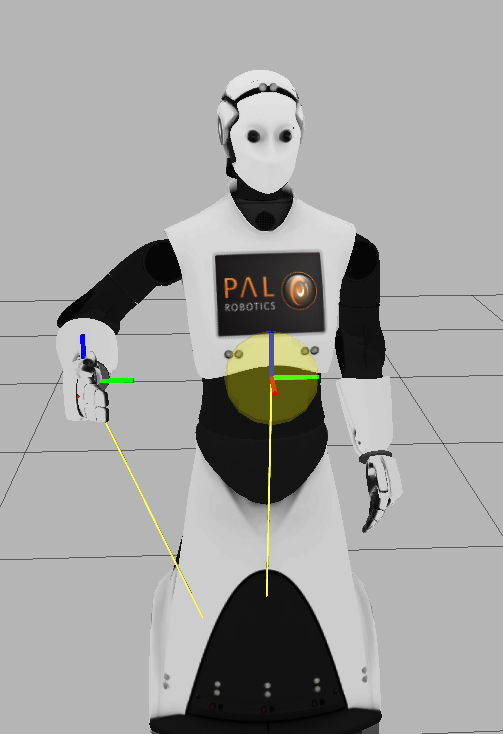
\includegraphics[width=0.23\textwidth]{../figures/arm_moves/1.png}
  	}
  	  \subfigure[]{
  		\label{fig:armmoves2} 
  		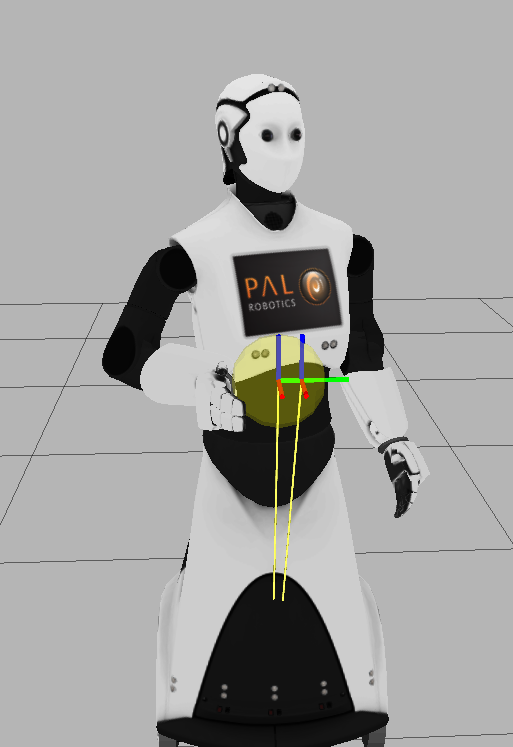
\includegraphics[width=0.23\textwidth]{../figures/arm_moves/2.png}
  	}
  	  \subfigure[]{
  		\label{fig:armmoves3} 
  		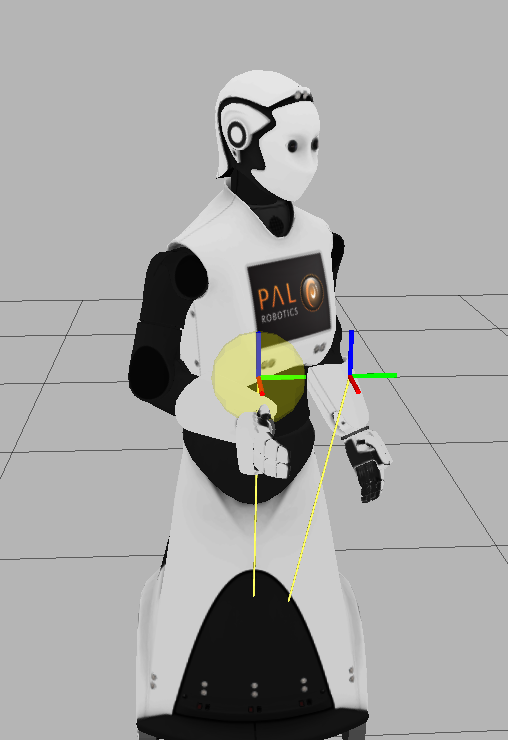
\includegraphics[width=0.23\textwidth]{../figures/arm_moves/3.png}
  	}
  	  \subfigure[]{
  		\label{fig:armmoves4} 
  		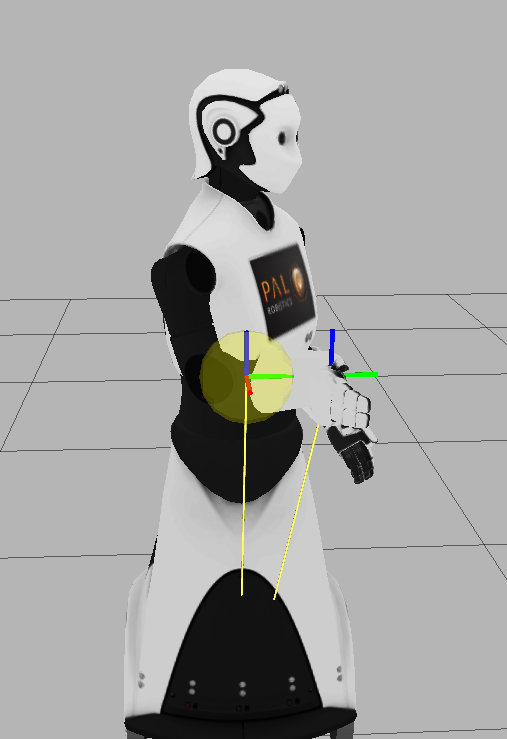
\includegraphics[width=0.23\textwidth]{../figures/arm_moves/4.png}
  	}
\caption{Sequence of screen shots for the predefined trajectory. The yellow ball represents the external obstacle, which has to be avoided. a) starting position b) collision avoidance gets activated as the obstacle boundary is reached c) alternate trajectory trying to minimize the error d) reaching desired position and collision avoidance is deactivated.}
    \label{fig:externarmmoves}
\end{figure}
In the sequence of screen shots, we can see that the arm is following the trajectory until the collision object is reached. At this point the collision avoidance task becomes part of the active set and the movement along the directional vector is limited. In order to minimize the error, an alternative path is solved and the obstacle is avoided.
A closer look at the trajectory is provided in figure \ref{fig:resultexternal}. It is remarkable, that the solver computes a different solution for the way back. Reasons for this might be the different starting configuration, where the HCOD fosters different joint movements at different times.
\begin{figure}[h!]
  \centering
    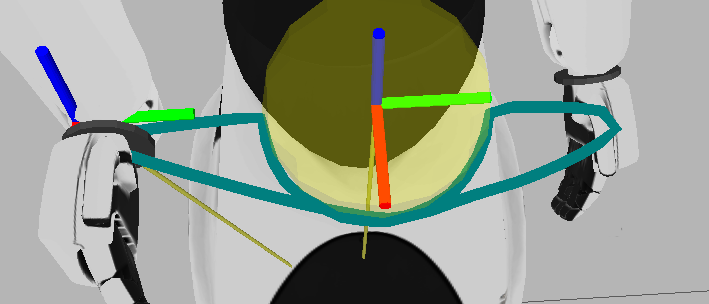
\includegraphics[width=0.6\textwidth]{../figures/arm_moves/result.png}
    \caption{Avoidance of external obstacle. In order to avoid the obstacle, yet minimizing the error towards the goal position, the movement yields along the collision object. The trajectory computed for the way back differs from the initial way. Reason for this are different starting positions and conditions. The HCOD solves the resulting equation system differently and fosters joint movements, which vary from the initial solution.}
    \label{fig:resultexternal}
\end{figure}

The distance over time is depicted in the plot below (Figure \ref{fig:externaldist}). Within this, we can see that the critical distance threshold $d_s$ is set to $0.1m$, which will not be violated. The distance between the obstacle and the wrist stays constantly over this specific safety zone.
\begin{figure}[h!]
  \centering
    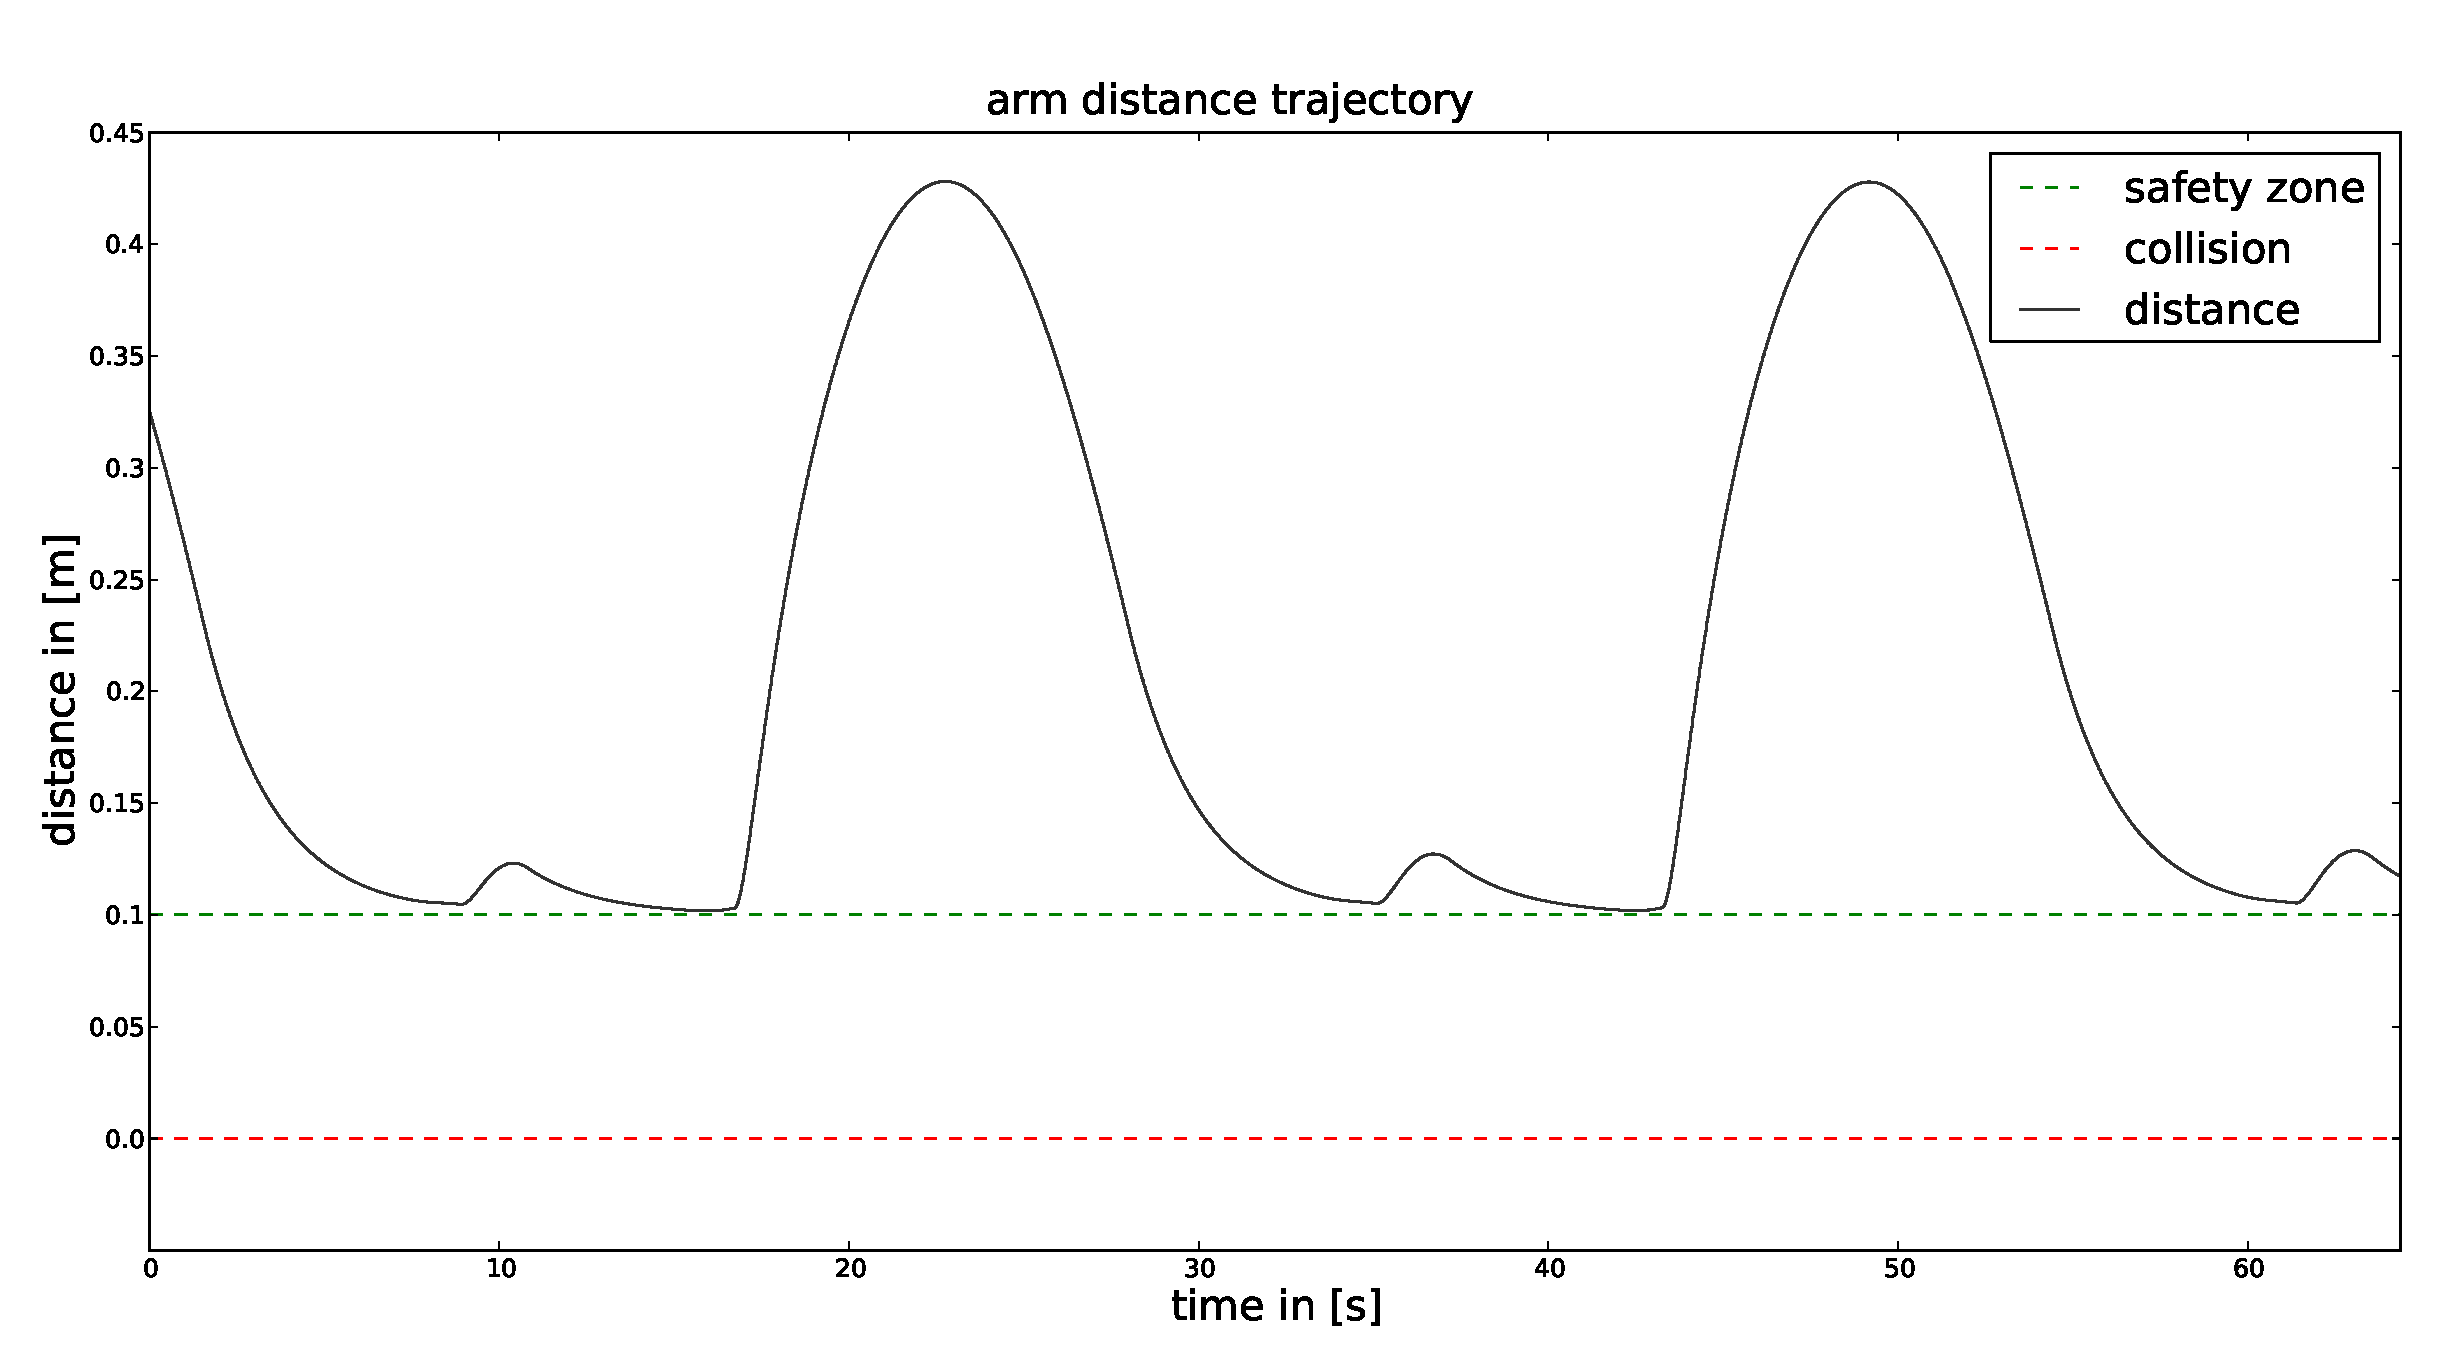
\includegraphics[width=\textwidth]{../figures/arm_moves/distance.eps}
    \caption{Distance plot over time. The distance stays constantly over the safety zone, which is specified as $0.1m$. The red line indicates a distance of 0, which is obviously the result of a full contact collision.}
    \label{fig:externaldist}
\end{figure}
When we look at the position trajectory in figure \ref{fig:externalposition}, we can also see the expected result. The displacement of the actual wrist position, compared to the desired position increases, when the distance converges towards the lower boundary. Furthermore, we can clearly see the attempt of the numerical solver to minimize the error to its best using non-constrained DOF. We can see this behavior around time $t=10s$. Since the desired trajectory is a sine wave in $Y$, the direction along this axis gets constrained, when the wrist moves closer to the obstacle. It can be seen, that the two DOF, such as $X$ and $Z$ are not constrained and can be used to minimize the error. We can see this in the plot, whenever there is an error value in $X$ and $Z$. 
\begin{figure}[h!]
  \centering
    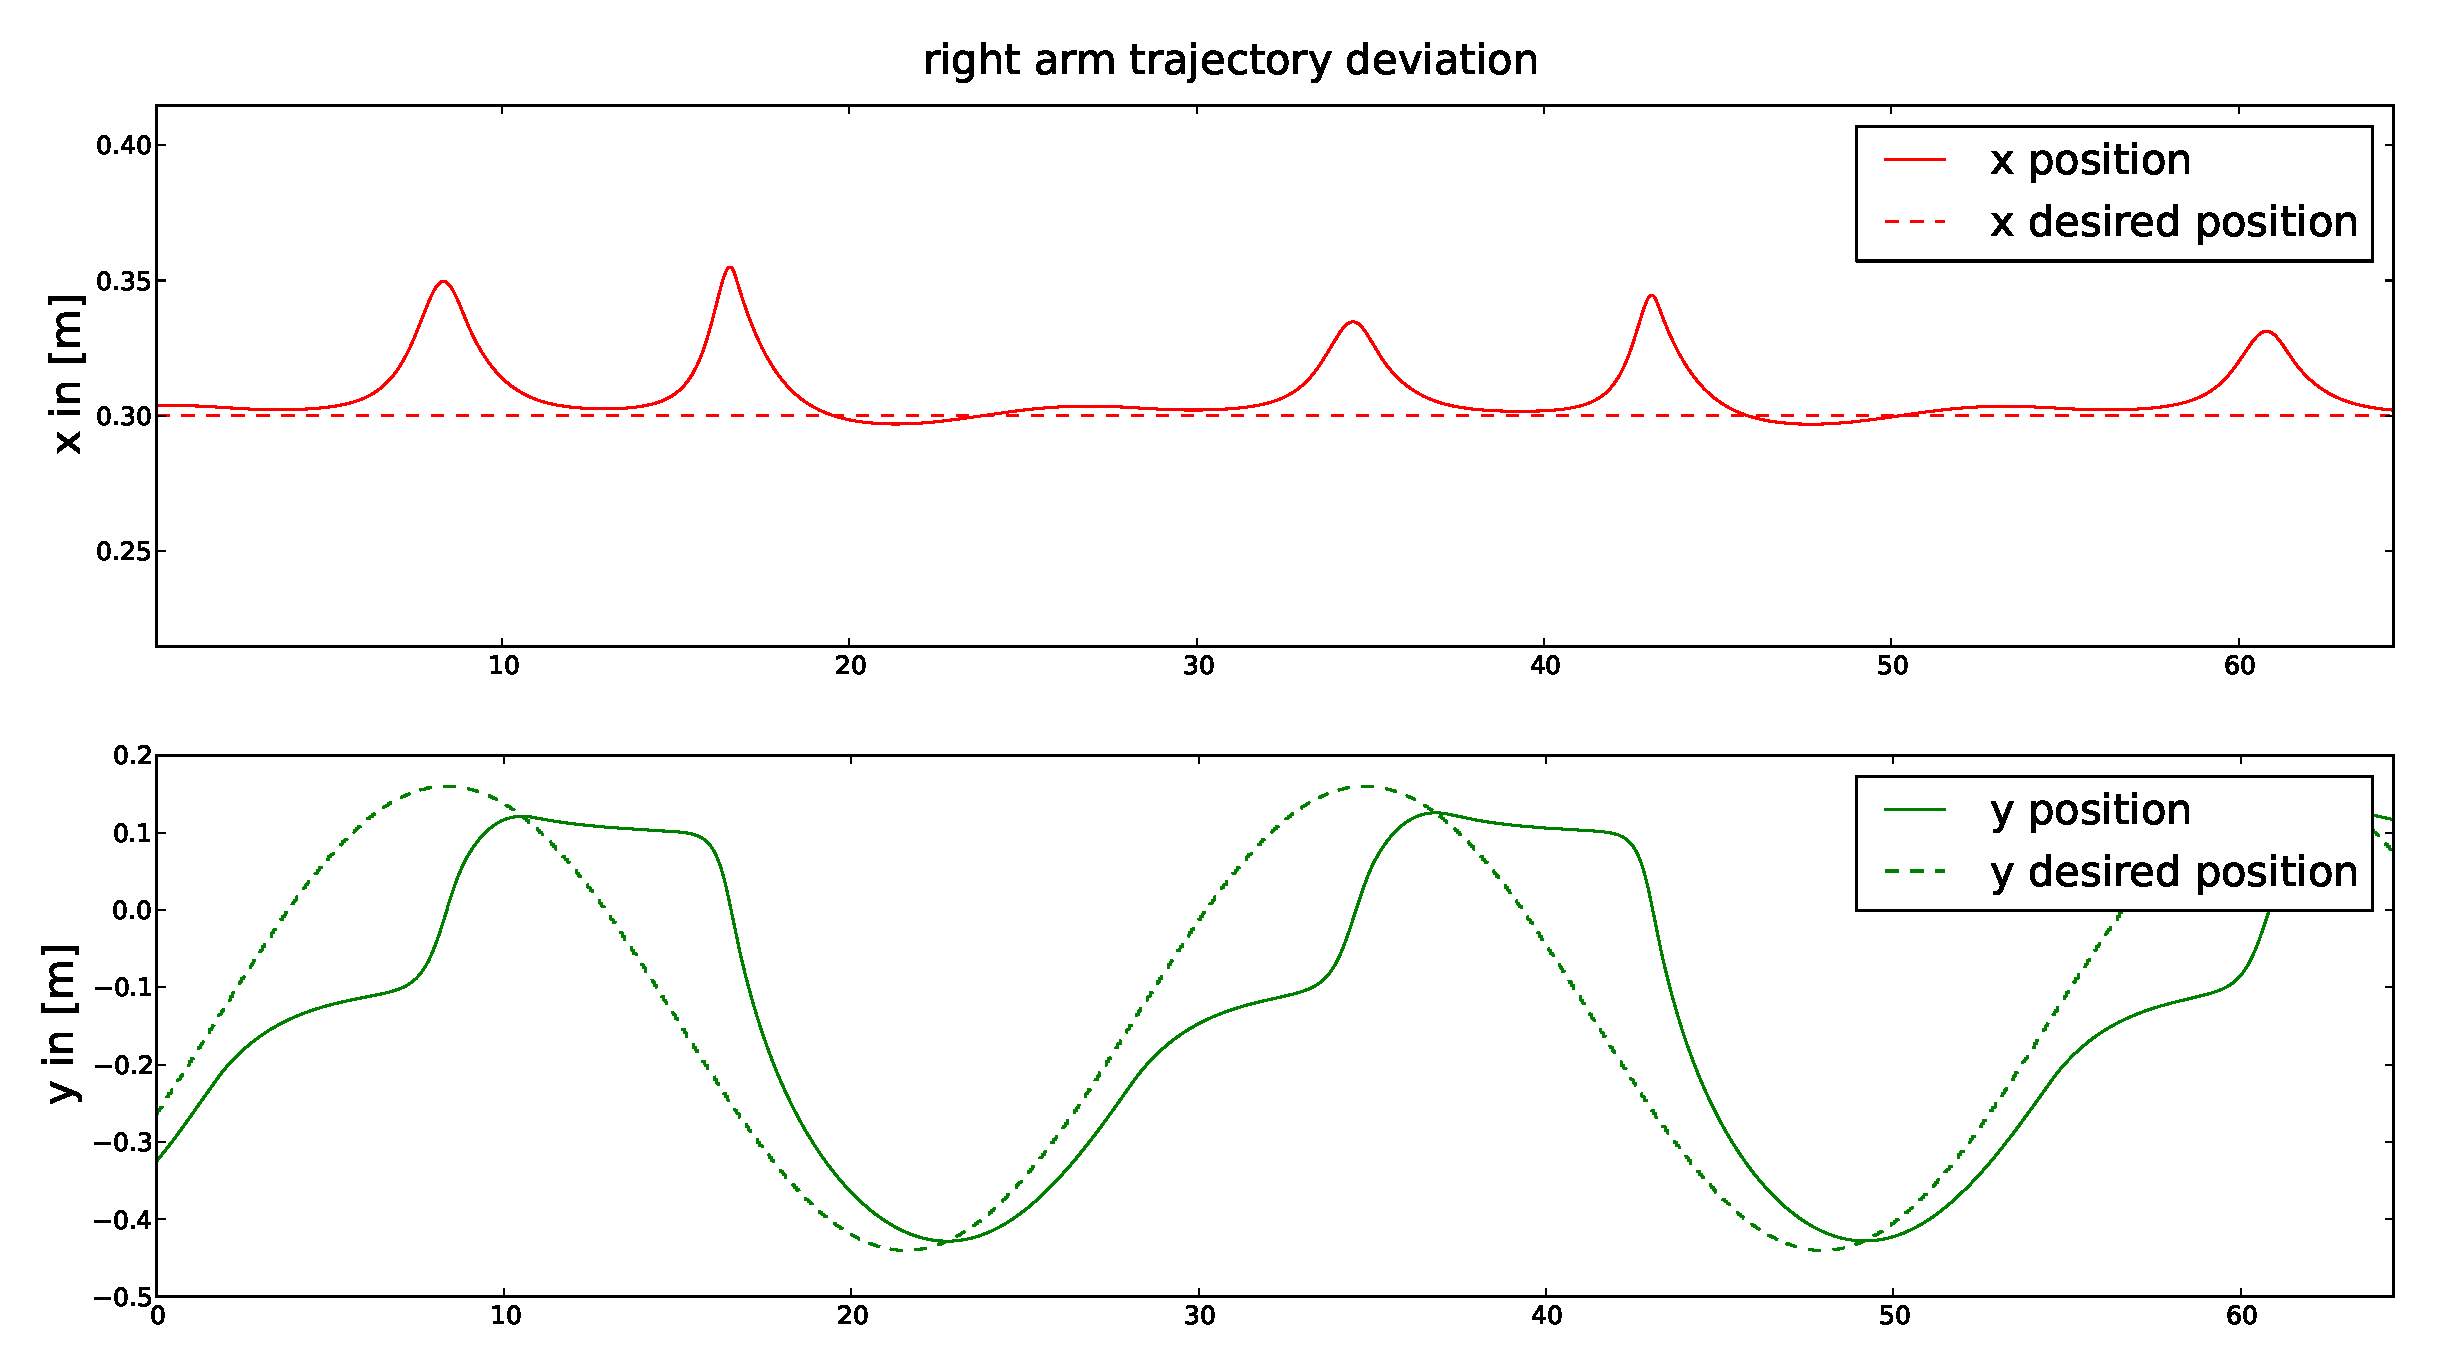
\includegraphics[width=\textwidth]{../figures/arm_moves/position1.eps}
    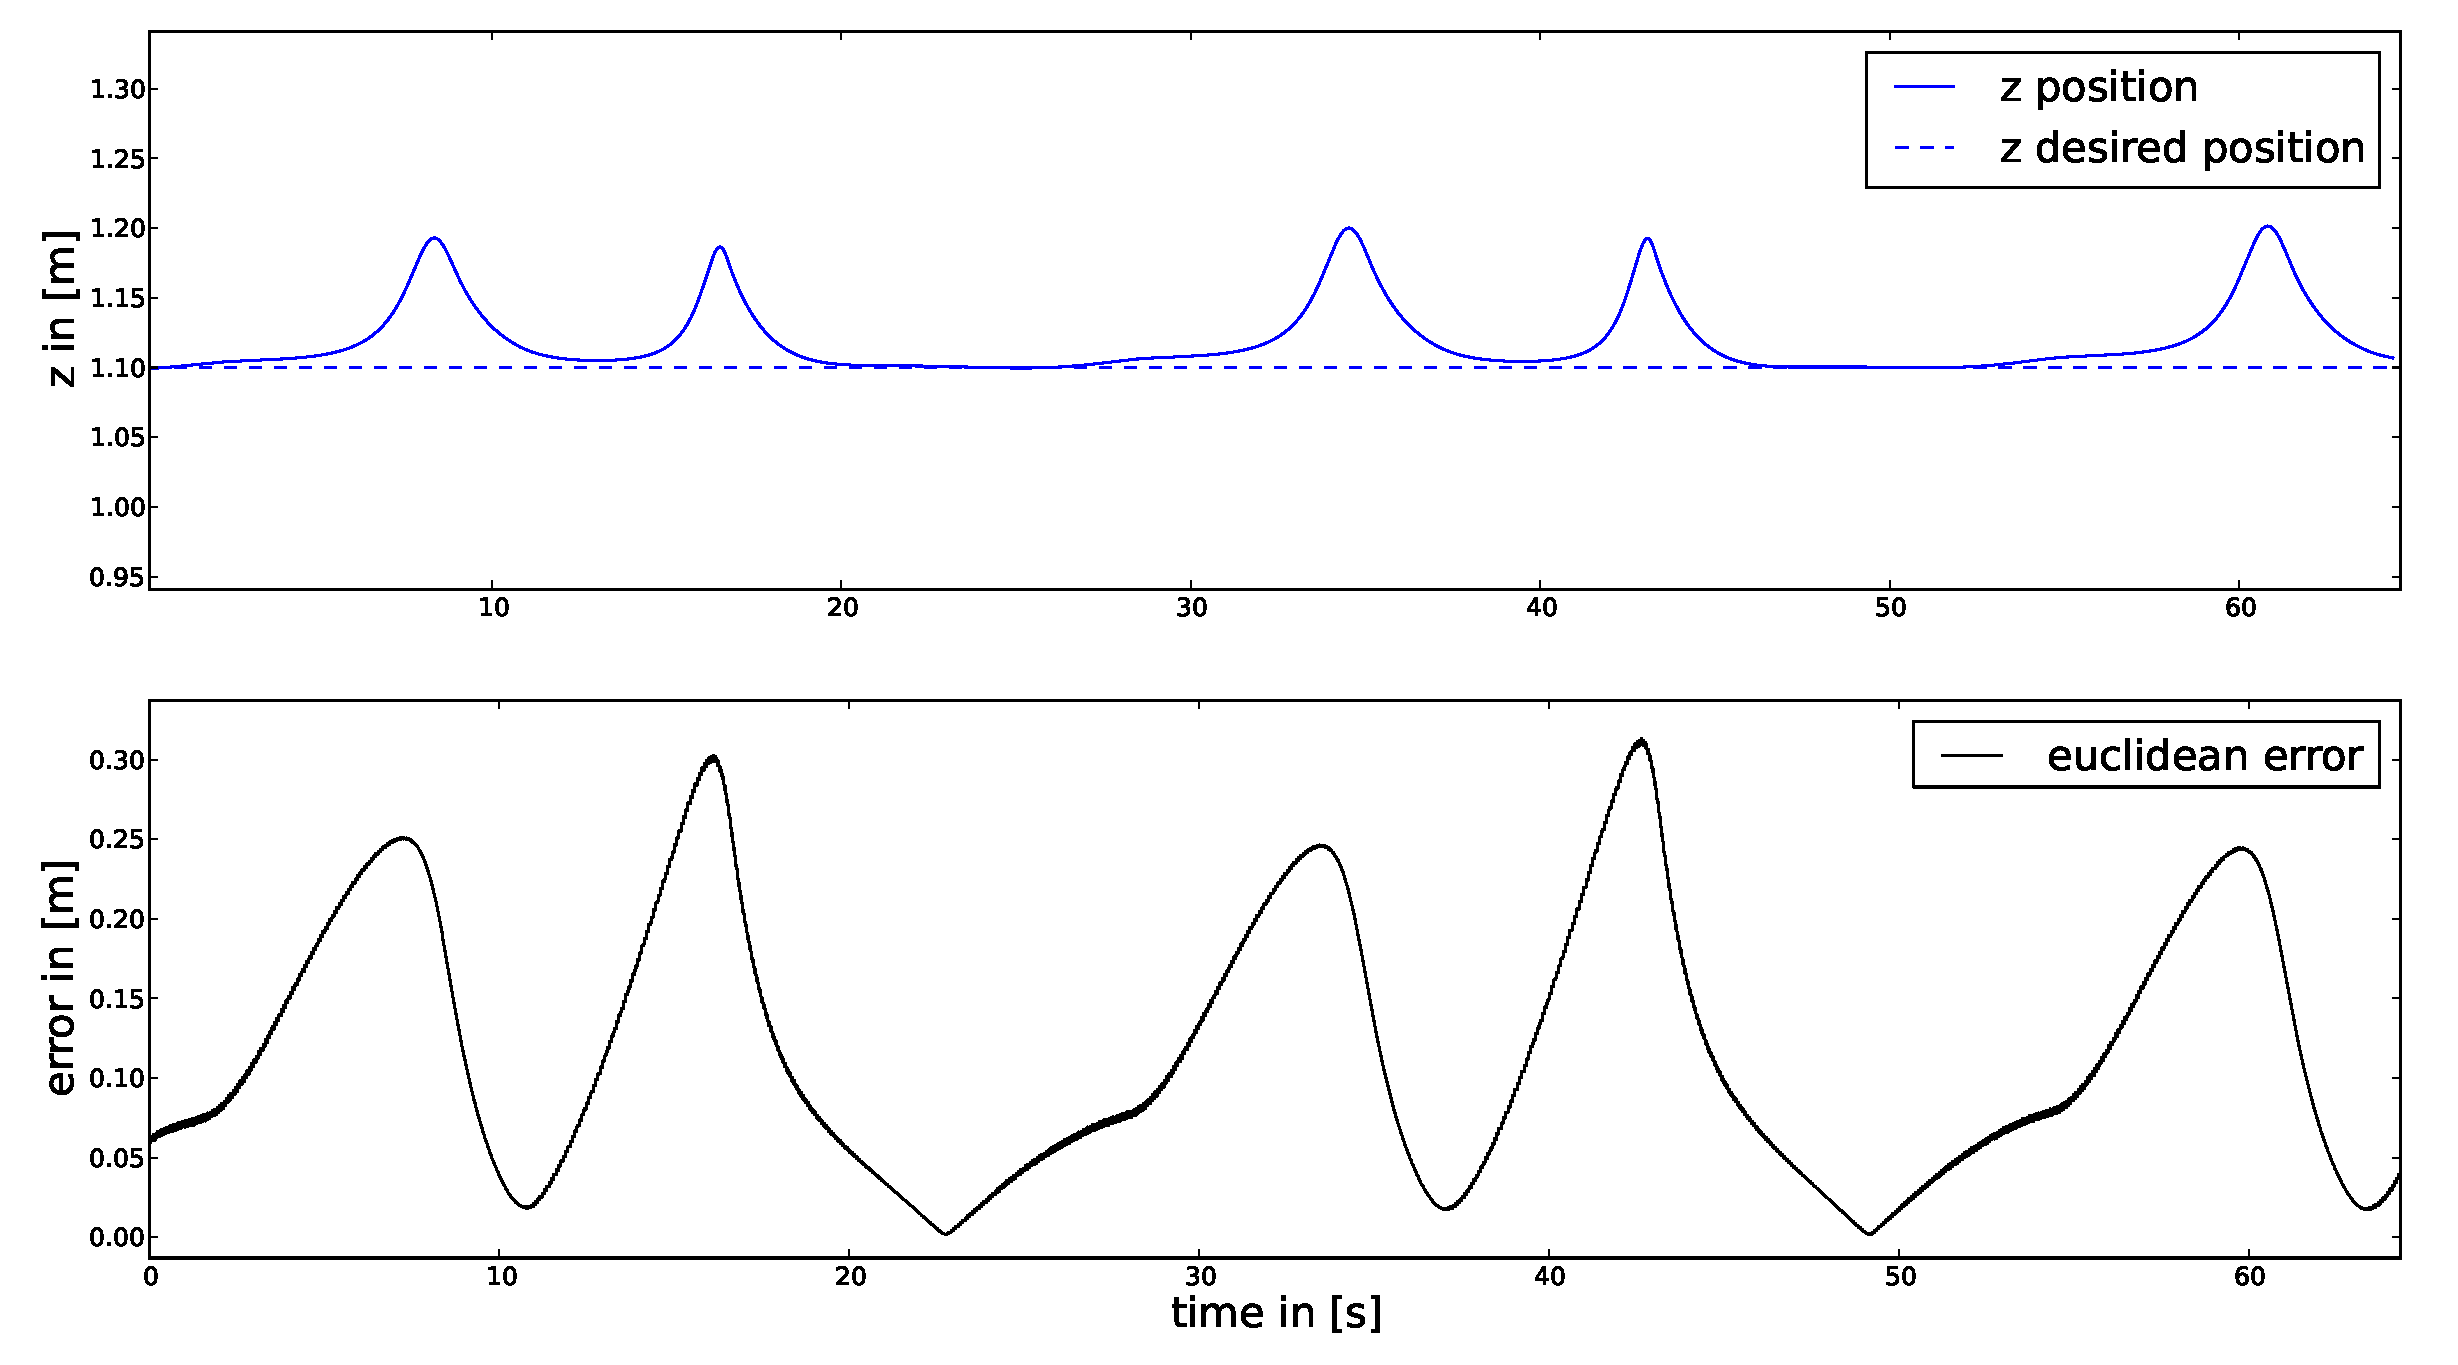
\includegraphics[width=\textwidth]{../figures/arm_moves/position2.eps}
    \caption{Position plot over time. Once a collision boundary is reached, the error increases as long as the obstacle constraint. Once the obstacle got avoided, the errors minimizes again as the goal position can be reached.}
    \label{fig:externalposition}
\end{figure}
\clearpage

\subsubsection*{Moving Object vs. Static Arm}
In the previous experiment, we moved the arm along a predefined trajectory, whereas the object was at a fixed position. In this experiment, we analyze the contrary setup. In the following, we keep the wrist at a static position and move the obstacle along a path, which would finally lead to a collision. We configured the velocity damping with a $\epsilon=10$. Equal to the previous test, $k$ was set to $10$ for the positioning task. Again, the executed trajectory is illustrated in the following sequence of graphics (figure \ref{fig:externobjectmoves}).
\begin{figure}[h!]
  \centering
  \subfigure[]{
  		\label{fig:objmoves1} 
  		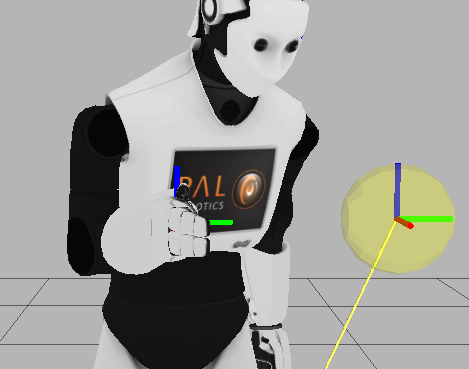
\includegraphics[width=0.23\textwidth]{../figures/object_moves/1.png}
  	}
  	  \subfigure[]{
  		\label{fig:objmoves2} 
  		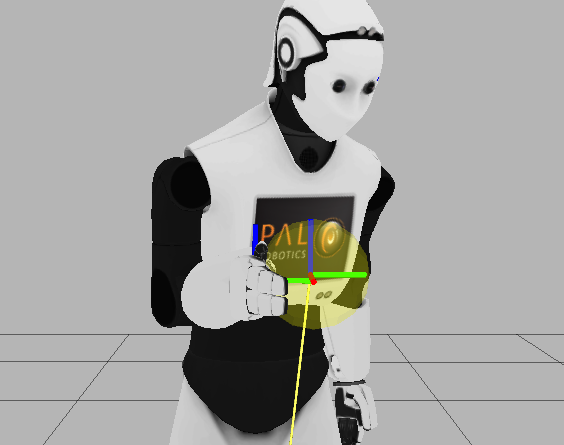
\includegraphics[width=0.23\textwidth]{../figures/object_moves/2.png}
  	}
  	  \subfigure[]{
  		\label{fig:objmoves3} 
  		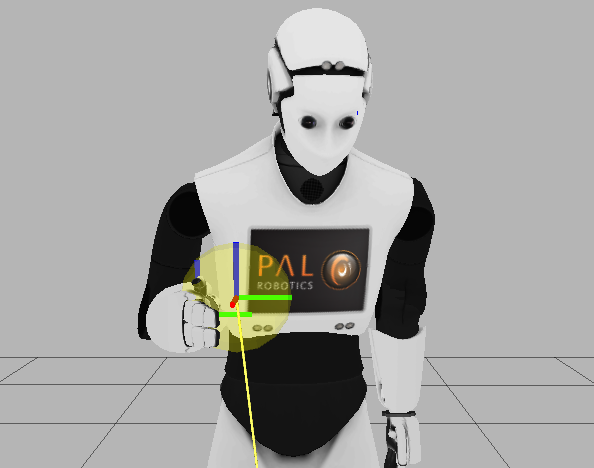
\includegraphics[width=0.23\textwidth]{../figures/object_moves/3.png}
  	}
  	  \subfigure[]{
  		\label{fig:objmoves4} 
  		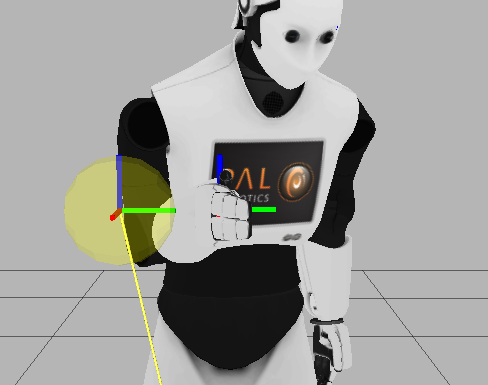
\includegraphics[width=0.23\textwidth]{../figures/object_moves/4.png}
  	}
  	  \subfigure[]{
  		\label{fig:objmoves5} 
  		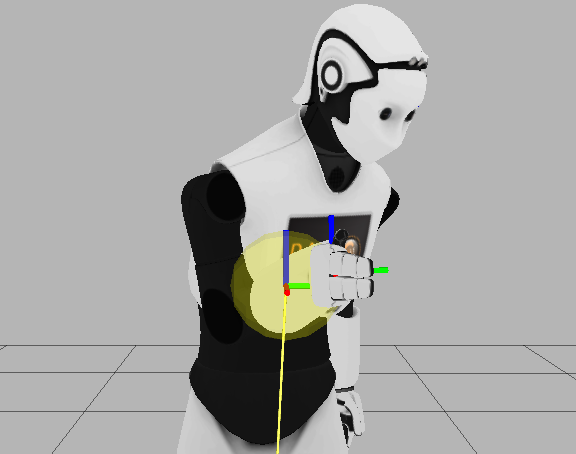
\includegraphics[width=0.23\textwidth]{../figures/object_moves/5.png}
  	}
  	  \subfigure[]{
  		\label{fig:objmoves6} 
  		\includegraphics[width=0.23\textwidth]{../figures/object_moves/6.png}
  	}
  	  \subfigure[]{
  		\label{fig:objmoves7} 
  		\includegraphics[width=0.23\textwidth]{../figures/object_moves/7.png}
  	}
  	  \subfigure[]{
  		\label{fig:objmoves8} 
  		\includegraphics[width=0.23\textwidth]{../figures/object_moves/8.png}
  	}
\caption{Sequence of screen shots for the predefined trajectory. The yellow ball represents the moving external obstacle, which is not allowed to collide with the arm. Figure a)-d) the obstacle is approaching the fixed arm from the right. When the collision boundary is reached, the arm gets pushed away from the obstacle. In order to minimize the emerging position error, the arm moves along the negative $X$ and $Z$ axis to avoid the obstacle. This is shown in c). Figure e)-h): The obstacle moves closes from the left side. The solution for avoiding the obstacle is a displacement along a positive $Z$ axis.} 
    \label{fig:externobjectmoves}
\end{figure}

Equally, as in the previous experiment, the collision avoidance possesses a higher priority compared to the positioning task of the right wrist, which has the lowest priority. Due to this alignment of the stack, the right wrist leaves its desired position, when the collision avoidance becomes active in figure \ref{fig:objmoves2}. The obstacle pushes the arm away from its desired position in \ref{fig:objmoves3}. However, the positioning task is still active, which minimizes the emerged error. The resulting minimization of the error leads into a displacement along the negative $X$ and $Z$ axis. Finally, the arm avoids the moving obstacle and resolves to its original desired position (figure \ref{fig:objmoves4}). 
\newpage
The second row (figure \ref{fig:objmoves5} - \ref{fig:objmoves8}) describes the counter movement, where the obstacles approaches the arm from the left side. To avoid the obstacle and to minimize the emerging error, the arm moves along a positive $Z$ axis. We can see the exact behavior of this description in diagram \ref{fig:objmovesposition}. 
\begin{figure}
  \centering
    \includegraphics[width=\textwidth]{../figures/object_moves/position1.eps}
    \includegraphics[width=\textwidth]{../figures/object_moves/position2.eps}
    \caption{Position plot over time. The obstacle gets avoided firstly by a negative movement in $X$ as well as $Z$. On the second approach, the avoidance happens by a movement in $Z$.}
    \label{fig:objmovesposition}
\end{figure}

The distance boundary $d_s$ was again set to $0.1m$. When we have a closer look at the distance development, we expect a similar behavior as in the previous test. The minimum boundary of $0.1$ is not allowed to get violated. 
Figure \ref{fig:objmovesdistance} provides information about the numerical exact distance. 
\begin{figure}
  \centering
    \includegraphics[width=\textwidth]{../figures/object_moves/distance.eps}
    \caption{Distance plot over time. The control gain are set to $\epsilon=10$, as well as $k=10$ for the positioning task. We can clearly see, that the safety distance is violated.}
    \label{fig:objmovesdistance}
\end{figure}

Contrary to our expectations, we see that the minimal boundary is violated. The minimal distance is not $0.1m$ but $0.872m$, which is a violation of approximately $13\%$. Furthermore, we can see a rather high frequent oscillation, once we hit the violation. 

In order to compensate for the violation as well as the oscillation, we retry the same experiments with a variation of the control gain $\epsilon$. 
Firstly, we set $\epsilon$ to a really high number such as $10000$ to see a tremendous chance, which can give possible insights about the reason for the violation. When we zoom in, we see the following result as depicted in figure \ref{fig:objmovesdistancek10000}.
\begin{figure}
  \centering
    \includegraphics[width=\textwidth]{../figures/object_moves/distancek10000.eps}
    \caption{Behavior of a huge control gain for the velocity damping task. Here, $\epsilon$ is set to $10000$. We can see that the violation still occurs, but in a smaller quantity. However, the resulting oscillation increases dramatically, which results in heavy discontinuities in the velocity domain.}
    \label{fig:objmovesdistancek10000}
\end{figure}

The figure in \ref{fig:objmovesdistancek10000} evinces a lower distance violation of $7\%, (0.937m)$ compared to the $13\% (0.872m)$ before. However, a violation still occurs with a heavily amplified oscillation, which contains huge discontinuities. These discontinuities in distance yield to a huge velocity, hence to a clearly noticeable shaking of the robot arm.

The second try to optimize this undesired behavior is to lower the gain. Thus, we redo the experiment with an $\epsilon$ of $0.01$. Again, the distance development over time is plotted below (see figure \ref{fig:objmovesdistancek1}).
\begin{figure}[h!]
  \centering
    \includegraphics[width=\textwidth]{../figures/object_moves/distancek001.eps}
    \caption{Behavior of a low control gain for the velocity damping task. Here, $\epsilon$ is set to $0.01$. We encounter a full collision and absolutely no attempt to avoid the obstacle. However, no discontinuities occur.}
    \label{fig:objmovesdistancek1}
\end{figure}

Figure \ref{fig:objmovesdistancek1} reveals the bottleneck of this method for avoiding obstacles. The control gain $\epsilon$ is set to $0.01$, which yields in no obstacle avoiding, since the minimal distance shrinks to $0.0m$, which is a full collision. Moreover, we can see that the right arm has a slow velocity, which yields, contrary to a control gain of $\epsilon=10000$,  into no heavy shaking of the robot. However, the velocity is way too small to avoid the obstacle in time.

Thus looking at the two variations, it becomes clearly that for this use case of accelerating a body part with zero initial velocity, special care has to be taken in gain tuning. When we want to provide service for any external velocities, the control gains have to be tuned according to the estimated velocity of the external obstacle. As we could see within this outcome, we have to find a trade-off between highly reactive body parts and lowest distance boundary violations. 

The important issue however, is that in all variations in $\epsilon$ the boundary gets violated. We discuss the nature of this in the next section \ref{sec:results}, where we analyze the reason this for in more detail.

\subsection{Self-Collision Avoidance}
As an enhancement of the collision avoidance task for external object, we examine now an avoidance of the robots body part itself. For the following concrete tests, we refer again to the capsule decomposition provided in table \ref{tab:capsules}. We consecutively test each group against each other. 
\begin{figure}[h!]
  \centering
    \includegraphics[width=0.48\textwidth]{../figures/closest_points_front.png}
    \includegraphics[width=0.48\textwidth]{../figures/closest_points_side.png}
    \caption{Visualization of the full collision matrix. Every collision pair is illustrated with its respective closest point pair onto the capsules surface. In this section, we examine all possible collision pairs with each other.}
    \label{fig:capsuleclosestpoint}
\end{figure}

We configure the velocity damping task according to each closest point pair, we take into consideration. Looking at figure \ref{fig:capsuleclosestpoint}, we illustrate the full collision matrix of possible colliding body parts with their respective closest points. In the remainder, we will test every point pair of this collision matrix. With this in mind, we test this collision matrix in a asynchronous, one-directional way. In particular, this means that, to begin with, we test the arms against the upper body as well as the head. As in the external collision avoidance, the arm tries to avoid the obstacle to its best. One-directional here denotes, that the arm avoids the upper body. However, the upper body does not avoid the arm. \\
Reasons for this decision were mainly to keep the number of constraints to a minimal configuration. Equally, the head and both torso links hold only one DOF, which brings just a little effect on avoiding 6 DOF of the arm. Furthermore, actively constraining the torso might have an bequeathing effect on the underlying wrist positioning task, since these links are commonly shared between both kinematic chains.
\begin{figure}[h!]
  \centering
  \subfigure[]{
  		\label{fig:armbody1} 
  		\includegraphics[width=0.148\textwidth]{../figures/arm_body/1.png}
  	}
  	  \subfigure[]{
  		\label{fig:armbody2} 
  		\includegraphics[width=0.148\textwidth]{../figures/arm_body/2.png}
  	}
  	  \subfigure[]{
  		\label{fig:armbody3} 
  		\includegraphics[width=0.148\textwidth]{../figures/arm_body/3.png}
  	}
  	  \subfigure[]{
  		\label{fig:armbody4} 
  		\includegraphics[width=0.148\textwidth]{../figures/arm_body/4.png}
  	}
  	  \subfigure[]{
  		\label{fig:armbody5} 
  		\includegraphics[width=0.148\textwidth]{../figures/arm_body/5.png}
  	}
  	  \subfigure[]{
  		\label{fig:armbody6} 
  		\includegraphics[width=0.148\textwidth]{../figures/arm_body/6.png}
  	}
  	\caption{Executed trajectory for the following self-collision experiment. We lead the arms into three possible collisions. Figure a)-b) would result in a collision with the lower torso, figure c)-d) equally with the upper torso. Finally, figure e)-f) illustrate a collision with the head. Thus, we describe a trajectory which alternates as a sine waves along $X,Y$ as well as a three step increase along $Z$.}
	\label{fig:armbody}
\end{figure}
\newpage
In the remainder of this section, a similar trajectory as the one depicted in figure \ref{fig:armbody} is executed. We can see, that we firstly set a goal position at the internal of the lower torso (figure a)-b)). We increase the height and repeat the same movement to provoke a collision with the upper torso (figure c)-d)). Finally, we repeat it equally with the head position (figure e)-f)). 

We can see the resulting positioning diagram in figure \ref{fig:selfcollisionposition}. At approx. $t=25s$, we shift the collision center from the lower torso to the upper torso. Similarly, we aim for colliding with the head at $t=70s$. We do not specify this position plot in more detail in any further experiment. We do this for simplicity reasons as the specified trajectory is mirrored for the left and right arm, which in the end results in a similar plot regardless the configuration of the positioning tasks.
\begin{figure}[h!]
  \centering 
     \includegraphics[width=\textwidth]{../figures/arm_body/position1.eps}
     \includegraphics[width=\textwidth]{../figures/arm_body/position2.eps}
    \caption{Positioning diagram of the applied trajectory for self-collision test. As we can see in the development of along the $Z$ axis, we increase the height in three steps: Lower torso, upper torso and head. We can assume an almost similar plot, independent whether a single arm or both are on the stack.}
    \label{fig:selfcollisionposition}
\end{figure}

\clearpage
\subsubsection*{Arms vs. Upper Body \& Head}
To begin with, we test the collision between one arm and the torso, which is quite likely to occur during common movements. Depending on the desired goal position, the minimal cost trajectory often leads through the torso. Thus, we start our examination on self-collision avoidance by repeatedly specifying a goal position for the arm, which is inside the upper body and head, respectively. 

The control gain for the two tasks of main interest are set to $\epsilon=10$ for the velocity damping as well as $k=10$ for the positioning task.   
A cumulated distance plot is displayed in \ref{fig:selfcollisiondistance}. We see that the violation zone gets not violated except from numerical errors. We can take the violations as numerical errors since the violation does not depend on $\epsilon$. We reproduced the experiment with different variations of $\epsilon$ with equally important results. Furthermore, looking at the numerical value of these violations, we can see a violation of $0.003m$, which essentially denotes a violation of $3mm$.  
\begin{figure}[h!]
  \centering
    \includegraphics[width=\textwidth]{../figures/arm_body/distance.eps}
    \caption{Distance plot over all tested collisions. We can see that except numerical issues, we do not have a tremendous violation of the safety zone. We can treat those violations are numerical instabilities as the violation does not depend on any variation of $\epsilon$. Furthermore, the maximum violation amounts to $0.003m$, which means $3mm$.}
    \label{fig:selfcollisiondistance}
\end{figure}

\subsubsection*{Full Collision Matrix}
We introduced the self-collision trajectories to be looped in a sine wave with an three-fold increase in $Z$. As seen before, this yields a satisfying result, with no noticeable violations. This approach of carefully designed goal positions, with all joints in a rather safe configuration, might serve as good-to-go for most of the robotic applications.

However, we have to review the fact, that the SoT is effectively a numerical solver. That being said, we have to remark, that no offline trajectory planning is done. This fact might yield in unknown or undesired positions and joint configurations. 
Therefore, we redo the above experiment with a full-featured collision matrix. This means, we configure the velocity damping with all items stated in table \ref{tab:capsules}. Hereby, we also introduce the collision between the two arms. 

Furthermore, in order to expand the working area and find unplanned joint configurations, we change the applied trajectory for the left and right arm by sine waves to be randomly changed in center position and the respective 3-dimensional amplitudes. Additionally, we increased the speed of the sine wave in order to move the robot with a realistic outcome speed.
The result of the distance for this experiment is shown in figure \ref{fig:selfcollisiondistancefull}. We can easily see, that the performance is equally satisfying as with in controlled environments. Equally, we can endorse the statement of numerical violations, since the noticeable small violations still occur, yet in the same quantitative magnitude. 
\begin{figure}[h!]
  \centering
    \includegraphics[width=\textwidth]{../figures/full/distance.eps}
    \caption{Distance plot of randomly changed trajectory of both arms. The collision avoidance takes all possible collision pairs into consideration. The result is equally satisfying as with predefined controlled movements.}
    \label{fig:selfcollisiondistancefull}
\end{figure}

\subsubsection*{Left Arm vs. Right Arm}
The result in the previous example, gave already a convincing outcome. We could assure, that all collisions (also in unexpected movements) are successfully avoided. Yet, we are mainly interested to position the hands in the most accurate way, meaning as close as possible to the desired position. Figure \ref{fig:selfcollisionfullerror} extracts exclusively the resulting euclidean error of the left and right arm. As we can easily see, the desired goal position is roughly getting reached. Obviously, the reason for this is that a collision occurs before reaching the desired goal. Thus, the hierarchy works as expected as the collision avoidance takes precedence over positioning one of the arms.  
\begin{figure}[h!]
  \centering
    \includegraphics[width=\textwidth]{../figures/full/error.eps}
    \caption{Extraction of the emerging euclidean error. The average error is visualized in green, the maximum error value in red. We can see that both arms have a remarkable non-zero average error.}
    \label{fig:selfcollisionfullerror}
\end{figure}

Let us have a closer look at the emerging error. The key values, such as average and maximum error value are comparably listed in table \ref{tab:errors}.
\begin{table}[h!]
\centering
\begin{tabular}{c c c} 
\hline
\multicolumn{3}{ |c| }{Euclidean Error [in m]} \\
\hline
\textbf{side} & \textbf{average} & \textbf{maximum} \\
\hline
left & 0.260 & 0.560 \\[0.2em]
\hline
right & 0.277 & 0.672 \\
\end{tabular}
\caption{error value extraction of plot displayed in figure \ref{fig:selfcollisionfullerror}}
\label{tab:errors}
\end{table}
Considering those values in the above table raises immediately the question about the hierarchy of the two low prioritized positioning tasks. For the above experiment, the left arm was placed over the right arm. Thus, the printed values are going along with this, yet probably not as meaningful as hoped.

To examine the priority conditions inside the hierarchy, we further test exclusively the avoidance between the two arms against each other. To do so, we define a counter directional trajectory in $Y$ for the two arms. We examine this particular movement twice, changing the priority of the left and right arm, respectively.

Prioritizing the right arm over the left arm, yields to the resulting movement indicated in figure \ref{fig:armrightoverleft}. We can see that according to the hierarchy level, the right\footnote{be aware that right and left are seen from the robots position. Thus, the sequence of pictures is flipped.} arm  strictly encounters a smaller error compared to the left arm.
\begin{figure}[h!]
  \centering
    \includegraphics[width=0.23\textwidth]{../figures/right_over_left/1.png}
    \includegraphics[width=0.23\textwidth]{../figures/right_over_left/2.png}
    \includegraphics[width=0.23\textwidth]{../figures/right_over_left/3.png}
    \includegraphics[width=0.23\textwidth]{../figures/right_over_left/4.png}
    \caption{Collision avoidance between both arms. The right arm takes precedence over the left arm.}
    \label{fig:armrightoverleft}
\end{figure}

Equally, we examined the inverse setup, having the left arm taking a higher priority than the right arm. Also, we display the sequence of movement in figure \ref{fig:armleftoverright}. As expected, the solution is exactly mirrored. The left arm describes a smaller error due to the higher priority.
\begin{figure}[h!]
  \centering
    \includegraphics[width=0.23\textwidth]{../figures/left_over_right/1.png}
    \includegraphics[width=0.23\textwidth]{../figures/left_over_right/2.png}
    \includegraphics[width=0.23\textwidth]{../figures/left_over_right/3.png}
    \includegraphics[width=0.23\textwidth]{../figures/left_over_right/4.png}
    \caption{Collision avoidance between both arms. The left arm takes precedence over the right arm.}
    \label{fig:armleftoverright}
\end{figure}

The actual remarkable outcome of this experiment is the fact that the higher priority task encounters a deviation of its desired position, although having precedence over the respective other one. In the latter, we will suggest to name this behavior \textit{Inversion of Hierarchy}. The synchronous collision avoidance influences the underlying tasks in a counter intuitive way, hence the name. As we can see in both displayed movements, the lower prioritized arm tries to avoid the higher prioritized arm to its best solution. At the same time though, the proximity between both arm rises until the lower priority encounters a clamping situation with zero velocity. This situation is equal to the distance violation we saw during the external collision avoidance tests. On the same hand, the higher prioritized arm still has to avoid every self-collision. For this reason, it also has to leave its desired position to keep the required distance threshold. Again, we refer to the next chapter \ref{sec:results}, where we verbosely analyze this outcome and provide mathematical reasoning.

\section{Results \& Discussion}\label{sec:results}

The overall outcome of the conducted experiments above is satisfying. We can see that, the applied method of decomposing the robots collision model into capsules yields to a smooth trajectory. Since we run those algorithms successful on the robot with $100Hz$, we can state, that the implementation is reasonably efficient. Moreover, we do not encounter any shaking of the robot body parts, even with a decent execution speed. With respect to the examined self-collision tests, we can also see a successful coverage of the complete body. Based on the placed capsules, the applied safety zone provides enough margin to bridge the transition between two adjacent capsules. 

For the collision avoidance, we firstly tested our introduced method against external collision objects. External objects get strictly avoided with a continuous and optimal displacement of the actuated body part as long as this has an initial and non-zero velocity. In case of an static actuated body part with zero velocity, we have to find a reasonable trade-off between oscillating and allowed violation of the specified safety zone. 

The self-collision avoidance represents the same task definition as for avoiding external objects, yet in a larger scale. For this, we configure the velocity damping task to avoid any collision with other body parts instead of one external object. This changes the task definition not to define one constraint inside the hierarchical solver but $\frac{1}{2}n^2$, where $n$ denotes the number of entries inside the collision matrix for all capsules. Since we run the self-collision avoidance in a one-directional manner, we only consider the upper triangle of this collision matrix, hence the division by 2. 

We state that all self-collisions can be avoided with great success. We encountered, besides a neglect able numerical error, that a collision avoidance based on closest point pairs of capsules yields to no self-collision. Equally important, we could execute the full collision matrix and additional lower prioritized tasks for positioning the end-effectors of both arms still in a decent speed. This generally justifies the application of this method to be sufficient enough to avoid (self-)collisions. On the same hand, it provides enough DOF to operate both arms in a reasonable speed and workspace.

\subsection{Violations of Safety Distance}
The above presented experiments show great success and give positive results for preventing self-collisions. Yet, we encountered that in certain cases, the safety zone gets violated. This misbehavior has the most impact, when the actuated body part is on a fixed position. In case of a moving collision object, the robot does not possess enough initial velocity to avoid the object in time. We similarly run into the same behavior for the self-collision avoidance, whenever clamping situations occur, which forces certain body parts to slow done until almost no velocity. 

The reason for this violation comes from the fact, that the applied method for avoiding collisions does not generate any velocity. In contrast to other popular methods such as repulsive forces, we produce no force rather than restricting the existing velocity not to proceed any further in the direction of possible collisions. For convenience, we present the velocity damping formulation of \ref{eqn:taskdampconstraint} again:
\begin{equation}\label{eqn:extaskdamping}
\vec{n}^T\vec{J(p,q)} \vec{\dot{q}} \geq - \epsilon \frac{d - d_s}{\Delta t} 
\end{equation}
A static position of the end-effector results in $\vec{\dot{q}} = 0$. The above formulation \ref{eqn:extaskdamping} thus turns into equation \ref{eqn:extaskdampingzero}, which is mathematically satisfied until $d_s$ reaches $d$. 
\begin{equation}\label{eqn:extaskdampingzero}
0 \geq - \epsilon \frac{d - ds}{\Delta t} 
\end{equation}
In the next step, $d_s$ becomes smaller than $d$, which implies an error calculation. Thus, the right hand side of the inequality in \ref{eqn:extaskdampinginverse} turns into a positive expression as $d - d_s$ becomes negative. At the same hand, the directional vector $n$ points now outside of the collision center. The overall expression flips the sign, so the inequality, which becomes finally:
\begin{equation}\label{eqn:extaskdampinginverse}
\vec{n}^T\vec{J(p,q)} \vec{\dot{q}} \leq  \epsilon \frac{\mathit{distance}}{\Delta t} 
\end{equation}
Note, that $distance$ here implies a negative value, since $d-d_s$ denotes a negative value here. This case actively produces a positive $\vec{\dot{q}}$ and the actuated end-effector moves. However, this heavily depends on the amplifier $\epsilon$. 
This being said, a velocity exists when there is an positive error between the desired and the actual position. A small $\epsilon$ just slightly amplifies the existing distance violation. Thus, a rather fast moving obstacle completely overruns the arm as shown in \ref{fig:objmovesdistancek1}, because the generated velocity is simply too small. 
On the contrary, a heavy amplification of epsilon might catapult the actuated arm far outside of the damping constraint. This deactivated the damping inside the solver and the underlying positioning task tries to minimize the displacement error. Thus, the robot moves again towards to collision center. This finally yields to heavy oscillations between the positioning task and velocity damping.


\subsection{Inversion of Hierarchy}
Situations which occur as in the experiment of colliding two arms show that the collision avoidance has a tremendous influence on the beneath placed and thus lower prioritized tasks against each other. As we can see in figures \ref{fig:armrightoverleft} and \ref{fig:armleftoverright}, the higher prioritized arm still encounters an error in position. Concretely explained on the example, where the right arm takes precedence over the left arm: When both arms come closer, the left arm navigates towards the torso. This movement will eventually result in a clamping situation, because of the possible collisions with the right arm. Clamping situations imply again a zero velocity. We call this behavior \textit{Inversion of Hierarchy}, since the lower priority positioning task has an remarkable impact on the above placed task. 

We could see in the experiment with a full collision matrix, that those situations occur but still do not yield in a collision. To overcome this behavior, a clearly defined gain tuning has to be done for each collision pair as well as the underlying positioning tasks. At the same time, the experiments were conducted with an equally set safety zone of $0.03m$. This might lead into undesired behavior, since certain collision pairs such as the upper arm and the torso are close by construction. Therefore, we implemented the self-collision setup based on a configuration file, where for each collision pair the specific set of parameters such as $\epsilon$ and $d_s$ are declared. 

		\chapter{Conclusion}
\label{chap:conclusion}

In this Master's thesis, we successfully implemented a complete solution for collision avoidance inside a hierarchical quadratic program. We integrated the Stack-of-Tasks efficiently inside a ROS-based environment and were therefore able to run it in real time on humanoid robots, such as REEM-H and REEM-C. \\

We implemented a reactive collision avoidance as an inequality constraint inside the quadratic program. Hereby, the velocity along the directional vector between the closest point pair of two collision objects is damped until a specified safety distance is reached. In order to avoid any singularities in calculating this closest point pair, we carried out a complete capsule decomposition for the robots collision model. The pseudo convexity of capsules lead to a smooth and moreover continuous trajectory of point pairs. We could prove, by various experiments, that the proposed solution is sufficiently stable to avoid any self-collision as well as deliver support for external collision objects. Thus, we could with great success accomplish all three goals of this work (see chapter \ref{item:goals}).

Equally, we freely admit, that the proposed method cannot be migrated as a out-of-the-box solution to different robots. Reasons for this is the strong dependency on the robot description file, which has to provide the support for capsules as a collision object. Furthermore, as we could see during the experiments, special care has to be taken for the control gain of the velocity damping. Those two configuration steps have to be calibrated for each individual robot.

The presented solution assures a safe execution of motion at all time. It ensures that all possible self-collisions are successfully avoided and the minimal distance threshold does not get violated (except numerical errors, which have to be taken into considerations). The collision avoidance thus is placed on a high level inside the hierarchy as a self-collision should never be violated. Since the velocity damping is realized as an inequality constraint, its result denotes a solution space. The suggested method provides a solution space, which is sufficiently large to not restrict the actual manipulation goals as long as they are outside the critical safety zone. It can thus be placed transparently on the top of the stack. It prevents all self-collision, but it flexible enough to not interfere the execution of beneath placed tasks.

The implementation for the humanoid robot from PAL Robotics REEM-H comprises a basic set of activated tasks on highest level, which are strictly necessary to allow a safe usage. On highest priority, joints limits have to be in range at all time in order not to physically harm the hardware of the robot. In particular, joint limits are meant as joint position as well as joint velocity limits. This is directly followed by the self-collision avoidance tasks. With this basic stack, a safe application can be performed on lower prioritized levels.

In general, the Stack-of-Tasks achieves very convincing performance in terms of whole body motion control. The execution speed of the inverse kinematic solver is by far ahead of any current implementations. This allows a smooth and application-driven usage of humanoid robots in a whole body control. The dynamic graph enables an easy \textit{plug-and-go} of input and output signals, which allows a straight-forward instantiation of fairly complex applications. \\
However, limitations arise on practical application aspects. Since the HCOD is a numerical solver, no look-ahead planning is done. This means, that even goal positions, which are clearly out of reach are solved to the best, minimizing the error between actual and goal position. This might lead to inappropriate behavior. Similarly, the DG operates in a constant control loop. Thus, emergency handling such as an immediate stop of the controller has to be handled with respect of this loop. 

		\chapter{Outlook}
\label{chapter:applications}

The presented method for self-collision avoidance is a passive task, which has only constraining purpose. It is not actively actuating any joints to achieve its goal. It is placed on top of the stack in order to monitor the movement of joints and prevent any collisions. 

However, the real impact of the SoT comes visible, when the stack is filled with inequality and equality constraints, and the robot is controlled with the whole body. Thus, in the following chapter, we briefly introduce applications, which we execute on REEM-H. With this, we want to demonstrate the capabilities of the SoT as well as provide an outlook of what is possible with current state of the art humanoid robots.

\subsection*{Object Tracking}
REEM-H possesses a stereo vision system as well as provides support with a Microsoft Kinect RDG-B sensor. With these vision systems we can easily implement an object tracking task. For this, we instantiate an entity, which captures the images from the vision system and provides the position of the object as an output signal. \\
Similarly, we instantiate a gaze task. A gaze task comprises a 2-dimensional plane $\vec{A}$, with a minimal distance $\vec{d}$ to this plane. The task is to keep the orientation of the attached joint $\vec{O}_i$ towards a point $\vec{p}$ on $\vec{A}$. 

Our implementation utilizes already existing components, which are successfully implemented on REEM-H. Related work regarding object recognition was done in \cite{bence}. We performed an object recognition with the help of Aruco markers (see figure \ref{fig:objectrecognition}), which allows an easy positioning of objects, where this marker is attached to.

\begin{figure}[h!]
  \centering
  \subfigure[Gaze Task Illustration]{
  		\label{fig:taskgaze} 
  		\includegraphics[width=0.4\textwidth]{../figures/gazetask.eps}
  	}
  	\hspace{2cm}
  \subfigure[Aruco Marker]{
  		\label{fig:arucomarker} 
  		\includegraphics[width=0.4\textwidth]{../figures/arucomarker.png}
  	}
	\caption{a) Illustration of a gaze task. The 2-dimensional plane $\vec{A}$, minimal distance $\vec{d}$ and a desired point $\vec{p}$. b) Example Arcuo marker, which is used to extract a full pose or position for various objects.}
    \label{fig:objectrecognition}
\end{figure}

A gaze task can be instantiated as a generic inverse kinematic task, which explicitly requires a Jacobian and a desired goal position for calculating the according error function. Since the vision system is attached at the head link, we plug the Jacobian of the head into the gaze task. The desired value \verb|P| corresponds to the position extraction of the Aruco marker.

\subsection*{Object Grasping}
We previously developed a task for tracking an object through a vision system. The only actuated joints hereby were the ones along the kinematic chain until the head. In order to achieve object grasping, we basically instantiate a positioning task for the end-effector of one arm. Similarly, to the gaze task, we plug the position of the Aruco marker as the desired goal position for this end-effector task. 

However, as in each grasping task, the main difficulty is the way the end-effector approaches the object. If we simply plug the marker position as the desired goal, we might hit the object with the manipulator, while reaching the position. We can overcome this issue by instantiating another gaze task. Contrary to the gaze task of the vision system, the place the gaze in the hand and have it orientate towards the marker. This forces the manipulator to approach the object with a correct grasping orientation.
\newpage
This setup of tasks can be already seen as whole body motion control, since multiple tasks partially share the same joints. Whenever this is the case, hierarchy race conditions occur. It might be dependent on the application, which task has more priority. In our implementation, we foster the head gaze to take precedence over the grasping task, since we want to ensure to have the object in the field of view.

\subsection*{Motion Retargeting}
As second application, we realized motion retargeting inside the SoT. Again, we could reuse existing solutions developed inside PAL \cite{marcus}. Motion retargeting is mainly used to realize teleoperations. Hereby, any RGB-D sensor, such as the Microsoft Kinect, captures a 3-dimensional image of a human and extracts the skeleton image. The idea of motion retargeting is then to translate the extracted joint positions of the human into joint positions of the according robot. Figure \ref{fig:teleop} illustrates the process.

\begin{figure}[h!]
  \centering
  \subfigure[Human movement]{
  		\label{fig:taskgaze} 
  		\includegraphics[width=0.37\textwidth]{../figures/teleop_real.png}
  	}
  \subfigure[Extracted skeleton]{
  		\label{fig:arucomarker} 
  		\includegraphics[width=0.20\textwidth]{../figures/kinect_skeleton.png}
  	}
  	  \subfigure[Translated movement on the robot]{
  		\label{fig:arucomarker} 
  		\includegraphics[width=0.37\textwidth]{../figures/teleop_reem.png}
  	}
	\caption{a) Image of the human movement b) Sketch of the extracted skeleton image c) Translated movement of the human into the robot.}
    \label{fig:teleop}
\end{figure}

We can flexibly realize teleoperations inside the SoT. The skeleton algorithms provides us with cartesian positions for each joint of the robot. Depending on how accurate we want the robot to imitate the movement of the human, we initiate a positioning task for each joint to track. Most often however, it is sufficient to track only the wrist and elbow positions, as the resulting movement of the remaining joints will be resolved quite similarly. 
\newpage
\subsection*{Dynamics}
Throughout this work, we completely worked inside a kinematic domain. This means, we resolved every task with a simple kinematic model in the form of 
\begin{equation}\label{eqn:kinematicmodel}
\vec{\dot{x}} = \vec{J}\vec{\dot{q}}
\end{equation}
This model can be shifted to a dynamics domain, which also considers velocities, inertia and masses to solve joint velocities. \cite{oscar} provides a complete solution to implement dynamics task inside the SoT. The equation in \ref{eqn:kinematicmodel} therefore becomes the Newton-Euler-Equation \cite{dynamics}:
\begin{equation}
\vec{M}(\vec{q}) \vec{\ddot{q}} + \vec{V}(\vec{\dot{q},q}) + \vec{g}(\vec{q}) = \tau
\end{equation}
		
		% -----------------------                                                                                                                                                  ----------------------------------------------------
		%
		% Appendix
		%
		% ---------------------------------------------------------------------------
		
%		\part*{Appendix}
%		\addcontentsline{toc}{part}{Appendix}
%		
%		\appendix %---------------------------------------
%		
%		\chapter{Detailed Descriptions}
%\section{Detailed Validation Results}
\label{chapter:DetailedDescriptions}
Here come the details that are not supposed to be in the regular text.
		
	


  \clearemptydoublepage
  
	\bibliography{bibliography/literature}
	
 
\end{document}

